%=================================================================
% This template is based on IMRT Latex template by Eric A. Mueller
%================================================================= 

\documentclass[10pt,twoside,a4paper]{report}

 \usepackage[mt,hs,english]{ethasl}   % New styles and commands
                                      % Options: 	bt/mt: Bachelorthesis/Masterthesis
                                      %						fs/hs: Fr�hlingssemester/Herbstsemester
                                      %						german/english: Deutsch/English

% \includeonly{}                      % Quick formatting
% \usepackage[draft]{graphicx}        % Quick formatting

 \usepackage{a4}                      % Paper size
 \usepackage[latin1]{inputenc}        % Keybord settings
 \usepackage{amsmath}                 % Additional math functionality
 \usepackage{amssymb}                 % Additional math functionality
 \usepackage{graphicx}                % EPS figures
 \usepackage[dvips]{epsfig}           % EPS figures
 \usepackage{float}                   % Placement of floating objects
 \usepackage{fancyhdr}                % Headings
 \usepackage{rotating}
 \usepackage{multirow}
 \usepackage{url}
 \usepackage{colortbl}
 \usepackage{ifpdf}
 \usepackage{caption}
\usepackage{subcaption}
 \usepackage{hyperref}

 \usepackage{hyperref}
 \usepackage{color}
 \definecolor{black}{rgb}{0,0,0}
 \definecolor{white}{rgb}{1,1,1}

 \definecolor{darkred}{rgb}{0.5,0,0}
 \definecolor{darkgreen}{rgb}{0,0.5,0}
 \definecolor{darkblue}{rgb}{0,0,0.5}

 \hypersetup{colorlinks
	,linkcolor=black
	,filecolor=black
	,urlcolor=black
	,citecolor=black
 }


 \ifpdf
	\usepackage[update]{epstopdf}
 \else
 \fi

% \usepackage{german}                  % German language
% \usepackage{ae}                      % German specials

%---------------------------------------------------------------------------

 \setlength{\parindent}{0em}                   % Disable parindent
 \rhead[\thepage]{\nouppercase{\rightmark}}    % Special headings
 \lhead[\nouppercase{\leftmark}]{\thepage}     % Special headings
 \cfoot{}                                      % Special headings

%---------------------------------------------------------------------------

 \title{Path Planning for Dynamic Maneuvers with Micro Aerial Vehicles}
 %\subtitle{bla bla bla}

 
 \studentA{Fabian Neusch\"{a}fer}
% \studentB{Student 2}
% \studentC{Student 3}
 
 

\supervisionA{Markus Achtelik}
\supervisionB{Michael Burri}
%\supervisionC{Supervisor C}
 

%===========================================================================
\begin{document}

%---------------------------------------------------------------------------
% Title page

 \maketitle
 \pagestyle{plain}
 \pagenumbering{roman}

%---------------------------------------------------------------------------
% Declaration of Originality

%\pagestyle{empty}
%% TODO Modify placeholders in declaration.tex
%%---------------------------------------------------------------------------
% Declaration of Originality
%
% TODO Add title, student first/last name, supervisor first/last name.

\section*{Declaration of Originality}

\vspace{1cm}

I hereby declare that the written work I have submitted entitled

\vspace{0.5cm}

% TODO Add title
\textbf{Path Planning for Dynamic Maneuvers with Micro Aerial Vehicles}

\vspace{0.5cm}

is original work which I alone have authored and which is written in my own words.\footnote{Co-authored work: The signatures of all authors are required. Each signature attests to the originality of the entire piece of written work in its final form.}

\vspace{1cm}

\textbf{Author(s)}

\vspace{0.5cm}

\begin{tabular}{ p{5cm} p{5cm} }
% TODO Add student first/last name
  First name & Last name \\
\end{tabular}

\vspace{0.5cm}

\textbf{Supervising lecturer}

\vspace{0.5cm}

\begin{tabular}{ p{5cm} p{5cm} }
% TODO Add supervisor first/last name
  First name & Last name \\
\end{tabular}

\vspace{1cm}

With the signature I declare that I have been informed regarding normal academic citation rules and that I have read and understood the information on 'Citation etiquette' (\url{http://www.ethz.ch/students/exams/plagiarism_s_en.pdf}). The citation conventions usual to the discipline in question here have been respected.

\vspace{0.5cm}

The above written work may be tested electronically for plagiarism.

\vspace{4cm}

\begin{tabular}{ p{5cm} p{1cm} p{5cm} }
  \cline{1-1} \cline{3-3}
  Place and date & & Signature \\
\end{tabular}

%---------------------------------------------------------------------------



%---------------------------------------------------------------------------
% Preamble

 %---------------------------------------------------------------------------
% Preface

%\chapter*{Vorwort}

%Bla bla \dots

 %\cleardoublepage

%---------------------------------------------------------------------------
% Table of contents

 \setcounter{tocdepth}{2}
 \tableofcontents

 \cleardoublepage

%---------------------------------------------------------------------------
% Abstract

%\chapter*{Zusammenfassung}
% \addcontentsline{toc}{chapter}{Zusammenfassung}

%Bla bla \dots

% \cleardoublepage



\chapter*{Abstract}
 \addcontentsline{toc}{chapter}{Abstract}

The goal of this master thesis is to develop a numerical robust trajectory planning algorithm for dynamic multi-copter flights in dense environments. The trajectory generated by this algorithm is represented by polynomials which are jointly optimized. The cost function of the optimization consists of the total trajectory-time as well as the total quadratic snap (second derivation of the acceleration). The inclusion of the snap into the cost function guaranties a trajectory without abrupt or expensive control inputs. \newline

Furthermore, the process of exploring the state space using the Rapidly-Exploring Random Tree (RRT) algorithm is embedded into the numerical robust algorithm. The sampling points oft the RRT (or RRT*) algorithm are then used as the nodes in the polynomial optimization.


\newpage
% \cleardoublepage

%---------------------------------------------------------------------------
% Symbols

%\chapter*{Symbolverzeichnis}\label{chap:symbole}
% \addcontentsline{toc}{chapter}{Symbolverzeichnis}
\chapter*{Symbols}\label{chap:symbole}
 \addcontentsline{toc}{chapter}{Symbols}

%\section*{Symbole}
%\section*{Symbols}
%\begin{tabbing}
% \hspace*{3cm} \= \kill
%  $\phi, \theta, \psi$ 		\> roll, pitch and yaw angle \\[0.5ex] 							
% \end{tabbing}

%\section*{Indizes}
%\section*{Indices}
%\begin{tabbing}
% \hspace*{1.6cm}  \= \kill
% $x$ \> x axis \\[0.5ex]
% $y$ \> y axis \\[0.5ex]
% 
%\end{tabbing}

\section*{Terms and Definitions}
\begin{tabbing}
 \hspace*{1.6cm}  \= \kill
jerk \> Derivation of acceleration \\[0.5ex]
snap \> Derivation of jerk \\[0.5ex]
vertex \> Fixed sampling point of a polynomial trajectory \\[0.5ex]
\end{tabbing}

%\section*{Akronyme und Abk�rzungen}
\section*{Acronyms and Abbreviations}
\begin{tabbing}
 \hspace*{1.6cm}  \= \kill
 ETH \> Eidgen\"{o}ssische Technische Hochschule \\[0.5ex]
 QP \>  Quadratic Programming\\[0.5ex]
 UAV \> Unmanned Aerial Vehicle \\[0.5ex]
RRT \> Rapidly-Exploring Random Tree\\[0.5ex]
ROS \> Robot Operating System\\[0.5ex]
\end{tabbing}

 \cleardoublepage

%---------------------------------------------------------------------------


 \pagestyle{headings}                 % Default headings
 \pagestyle{fancy}                   % Special headings
 \pagenumbering{arabic}

%---------------------------------------------------------------------------
% Chapters

 
\chapter{Introduction}\label{sec:introduction}

\section{State of the Art}\label{sec:state}

A lot of research has been performed in the field of Unmanned Aerial Vehicles (UAV) in the last years leading to a strong improvement in trajectory planning \cite{he} as well as in control (\cite{colling}, \cite{hehn}).  Another field of research is machine learning \cite{lup} which is suitable to enhance the performance of aerobatic maneuvers but seems to have a downside regarding motion planning and trajectory generation in dense environments. \newline

Speaking of trajectory planning, there are two different strategies which are pursued. On the one hand, the geometric and the temporal planning are decoupled  \cite{bou}, on the other hand geometric and temporal information are coupled and the trajectory is the result of a minimization problem. For the coupled problem one can make use of the differential flatness of a quadrocopter to derive constraint on the trajectory. A cost function which could be the total trajectory-time \cite{hehn} or the total snap \cite{mellinger} can be formulated. \newline


%Then formulate a cost-function which could be the trajectory-time \cite{hehn} or the total snap \cite{mellinger} (second %derivation of acceleration). \newline

Another aspect of planning is exploring the state space in the first place. A strong tool to do so are incremental search techniques as for instance the A* \cite{lik} or the RRT* algorithm \cite{richter}. The sampling points of the solution of the incremental search can then be used as the nodes for the polynomial optimization.

\section{Quadratic Programming}\label{sec:quadratic}

As mentioned above, the snap can be used as the cost function in trajectory optimization. Regarding snap minimization, Quadratic Programming (QP) is a powerful tool.

\subsection{Constrained Quadratic Programming}

QP is a special case of an optimization problem in which a quadratic function $f(x)$ is optimized with respect to its optimization variables (which are represented with the vector $x$ in equation \ref{equ:quadratic})

\begin{equation}
 f(x)  = \frac{1}{2} \cdot x^T Q x + c^T x 
\label{equ:quadratic}
\end{equation}

The optimization can be performed under linear constraints on the optimization variables. The linear constraints can be divided in two groups. \newline

 For one thing there are the inequality constraints

\begin{equation}
A  x \leq b
\label{equ:inequalityConstraintsQP}
\end{equation}

where the vector $b$ contains the inequality constraints. For another thing there are the equality constraints

\begin{equation}
E  x = d
\end{equation}

where the vector $d$ contains the equality constraints. In case there are only equality constraints, the solution to the QP is given by the linear system in equation \ref{equ:equality} :



% Whereas a distinction between equality($ E\mathbf{x} = \mathbf d $) and inequality constraints ($ A\mathbf{x} \leq \mathbf b $) has to be made. 
%In case there are only equality constraints, the solution to the QP is given by the linear system in equation \ref{equ:equality} :


\begin{equation}
\begin{bmatrix}
   Q & E^T \\
   E & 0
\end{bmatrix} 
\cdot
\begin{bmatrix}
   \mathbf x \\
   \lambda
\end{bmatrix}
= 
\begin{bmatrix}
   -\mathbf c \\
   \mathbf d
\end{bmatrix}
\label{equ:equality}
\end{equation}


where $\lambda$ is a set of Lagrange multipliers and $c$ is the linear term of the cost function in equation \ref{equ:quadratic}. \newline

The constrained QP gets ill-conditioned for a large number of optimization variables which lead to large matrices. The performance of the constraint QP deteriorates even more if the matrices are sparse. This particular case often appears in polynomial optimization for high order polynomials where some polynomial coefficients are close to zero. \newline

To reduce the number of optimization variables, and therefore the size of the matrices, the constrained QP with equality constraints can be converted into a numerical robust unconstrained QP. This is one of the goals of this master thesis.

\subsection{Unconstrained Quadratic Programming}

For the unconstrained QP the equality constraints $E \mathbf{x} = \mathbf{d}$ resp. $\mathbf{x} = E^{-1} \mathbf{d}$ are embedded into the quadratic cost function from equation \ref{equ:quadratic} resulting in equation \ref{equ:quadratic_unconstrained}:

\begin{equation}
 f(d)  = \frac{1}{2} \cdot d^T  E^{-T}  Q  E^{-1}  d + c^T  E^{-1} d
\label{equ:quadratic_unconstrained}
\end{equation}

Since the vector $x$ is replaced by $E^{-1} d$ and $E$ is a constant matrix, the new optimization variables are now stored in the vector $d$. \newline
 
%Referring to polynomial trajectory optimization, the vector $x$ containing the polynomial coefficients is now replaced by the vector $d$ containing the endpoint derivatives and the mapping matrix $E$. In other words, the polynomial coefficients are no longer the optimization variables but the free endpoint derivatives are optimized. Furthermore the polynomial trajectory optimization does not have a linear term $c^T \mathbf{x}$. Hence Equation \ref{equ:quadratic_unconstrained} can be simplified to:  

If the cost function defined in equation \ref{equ:quadratic} does not have a linear term, i.e. the vector $c$ is equal to zero, equation \ref{equ:quadratic_unconstrained} can be simplified to:

\begin{equation}
 f(d)  = \frac{1}{2} \cdot d^T  E^{-T}  Q  E^{-1}  d 
\label{equ:quadratic_simple}
\end{equation}

If we are not interested  in the cost itself but only in the optimization variables stored in $d$, the constant multiplier $1/2$ can be dropped:

\begin{equation}
 f(d)  = d^T  E^{-T}  Q  E^{-1}  d 
\label{equ:quadratic_short}
\end{equation}

The theoretical derived equation \ref{equ:quadratic_short} will be compared to to multidimensional cost function in equation \ref{equ:uncon_cost}. Equation \ref{equ:uncon_cost} establishes a connection between the numerical advantages of a unconstrained QP and the polynomial coefficients representing a trajectory.













 \cleardoublepage
 \chapter{Polynomial Trajectory Optimization}\label{sec:trajectory}


\section{Polynomial Trajectory}\label{sec:polynomial}

Regarding the differentiability of polynomials, they are a profound choice to represent a trajectory. Especially for the use in a differentially flat representation of the UAV dynamics. (Flatness in the proper sense of system theory means that all the states and inputs can be expressed in terms of the flat output and a finite number of its derivative).
Furthermore, the differentiability of polynomials enables the possibility to check the derivatives of the trajectory for bounding violations to avoid input saturation. This saturation-check can be performed during trajectory optimization and therefore guarantees the feasibility of the resulting trajectory.

\section{Optimization}\label{sec:optimization}

The goal of this master thesis is to optimize a trajectory which passes through waypoints (also called vertices or nodes) which are defined in advance. This waypoints can be chosen manually or by a path-finding algorithm such as RRT* which will be discussed in chapter \ref{chap:RRT}.
Furthermore, not only the waypoints (i.e. the position) can be fixed in advance but also its derivatives (such as speed, acceleration etc.). The position and its derivatives are then utilized as the equality constrains for a QP (explained in Section \ref{sec:quadratic}).

\subsection{Cost Function}\label{sec:cost}

Optimization for the purpose of trajectory planning means to minimize a cost function. The cost function in this case is a combination of temporal and geometric cost. The geometric cost penalizes the square of the derivatives of the trajectory. In this master thesis the geometric cost is represented by the squared snap which guarantees a trajectory without abrupt  control inputs. \newline
The temporal cost is simply the total trajectory time multiplied by a user chosen factor $k_T$ which determines the aggressiveness of the resulting trajectory. The impact of  $k_T$  can be seen in equation \ref{equ:total_cost} which represents the combined geometric and temporal cost. \newline

To express the geometric cost in a compact way one can utilize the Hessian matrix $Q$. The Hessian matrix is defined as a squared matrix of second-order partial derivatives which follows from differentiation a function with respect to each of its coefficients, in this instance the polynomial coefficients. The geometric cost function $J(T)$ for one segment with the duration $T$ can now be written as

\begin{equation}
J(T)  = p^T \cdot Q(T) \cdot p
\end{equation}

where $Q(T)$ is the Hessian matrix for a fixed segment time $T$. $p$ is the vector containing the coefficients of the polynomial trajectory. \newline

If the trajectory consists of more than one segment the Hessian matrix has to be extended to a block-diagonal matrix. The geometric cost function for multiple segments with fixed but individual segment times $T_i$ can be written as

\begin{equation}
J(T) =
\begin{bmatrix}
   p_1 \\
\vdots \\
  p_n
\end{bmatrix}^T
\cdot
\begin{bmatrix}
   Q_1(T_1) &  &  \\
    & \ddots &  \\
   & & Q_n(T_n)
\end{bmatrix} 
\cdot
\begin{bmatrix}
   p_1 \\
\vdots \\
  p_n
\end{bmatrix}
\label{equ:cost}
\end{equation}


\subsection{Polynomial Optimization as a Constrained QP}

The cost function in equation \ref{equ:cost} has to be minimized under constrains since we want to fix things like start or end position. In a first intuitive approach the constraints on the endpoint derivatives are utilized in a constrained QP. Therefore, a mapping matrix $E$ between endpoint derivatives and polynomial coefficients is needed. The resulting equality constraint for the $i^{th}$ segment can be written as

\begin{equation}
E_i \cdot p_i = d_i
\label{equ:mapping}
\end{equation}

where $p$ is the vector containing the polynomial coefficients and $d$ is the vector containing the endpoint derivatives. Regarding the total number of segments of the trajectory, equation \ref{equ:mapping} can be written in matrix form:

\begin{equation}
\begin{bmatrix}
   E_1 &  &  \\
    & \ddots &  \\
   & & E_n
\end{bmatrix} 
\cdot
\begin{bmatrix}
   p_1 \\
\vdots \\
  p_n
\end{bmatrix}
=
\begin{bmatrix}
   d_1 \\
\vdots \\
  d_n
\end{bmatrix}
\end{equation} 

The constrained QP is suitable for a small amount of segments but gets ill-conditioned for a large amount of segments and therefore large matrices. Especially if there are matrices which are close to singularity and have coefficients which are close to zero, the constrained QP can get numerical unstable.

\subsection{Polynomial Optimization as a Unconstrained QP}\label{sec:polynomialQP}

To avoid the numerical instability of a constrained QP the optimization problem is converted into a unconstrained QP. To achieve this, the polynomial coefficients $p_i$ from equation \ref{equ:cost} have to be substituted by the endpoint derivatives $d_i$ which are now the new optimization variables. The cost function of the unconstrained QP can now be written as 

\begin{equation}
J =
\begin{bmatrix}
   d_1 \\
\vdots \\
  d_n
\end{bmatrix}^T
\cdot
\begin{bmatrix}
   E_1 &  &  \\
    & \ddots &  \\
   & & E_n
\end{bmatrix} ^{-T}
\cdot
\begin{bmatrix}
   Q_1 &  &  \\
    & \ddots &  \\
   & & Q_n
\end{bmatrix} 
\cdot
\begin{bmatrix}
   E_1 &  &  \\
    & \ddots &  \\
   & & E_n
\end{bmatrix} ^{-1}
\cdot
\begin{bmatrix}
   d_1 \\
\vdots \\
  d_n
\end{bmatrix}
\label{equ:uncon_cost}
\end{equation}

where $Q_i$ is the Hessian matrix according to the $i^{th}$ segment time $T_i$.\newline

As mentioned above, the endpoint derivatives are the new optimization variables. Due to the equality constrains some of the endpoint derivatives are already specified consequently reducing the number of optimizations variables. Expediently, the endpoint derivatives are divided in fixed derivatives $d_f$ and unspecified derivatives $d_p$ and then reordered using the matrix $C$ which consists of zeros and ones. After reordering the endpoint derivatives equation \ref{equ:uncon_cost} can be rewritten as

\begin{equation}
J =
\begin{bmatrix}
   d_f \\
  d_p
\end{bmatrix}^T
\underbrace{C^T E^{-T} Q E^{-1} C}_\text{R}
\begin{bmatrix}
   d_f \\
  d_p
\end{bmatrix}
\label{equ:R_cost}
\end{equation}

where the product of the reordering matrix $C$, the mapping matrix $E$ and the Hessian matrix $Q$ can be expressed as a single Matrix $R$. The matrix $R$ for his part can be divided into four submatrices according to the fixed and unspecified endpoint derivatives which modifies equation \ref{equ:R_cost} as follows:

\begin{equation}
J =
\begin{bmatrix}
   d_f \\
  d_p
\end{bmatrix}^T
\begin{bmatrix}
   R_{ff} & R_{fp} \\
  R_{pf} & R_{pp}
\end{bmatrix}
\begin{bmatrix}
   d_f \\
  d_p
\end{bmatrix}
\label{equ:Rxx_cost}
\end{equation}

Partially differenting equation \ref{equ:Rxx_cost} with respect to the unspecified derivatives $d_p$ and equate it to zero yields the optimized/minimized unspecified derivatives $d_p^*$ 

\begin{equation}
d_p^* = - R_{pp}^{-1} \cdot R_{fp}^T \cdot d_f
\label{equ:dpstar}
\end{equation}

as a function of the fixed derivatives $d_f$ and two of the submatrices ($R_{pp}, R_{fp}$) of $R$.


\section{Initial Solution}\label{sec:initialSolution}

Equation \ref{equ:dpstar} can now be used to compute the initial solution. As can be seen in equation \ref{equ:uncon_cost}, the Hessian matrix for the  $ i^{th}$ segment $Q_i$ depends on the segment time $T_i$. Thus, all the segment times have to be defined in advance. For the initial solution the segment times are calculated based on the Euclidean distance $d_{norm}$ and on the user specified maximal speed ($v_{max}$) and maximal acceleration ($a_{max}$). \newline

Basically the segment time is determined by the term $d_{norm}/v_{max} \cdot 2$ which is twice the time the UAV would need for a segment by flying the whole distance at maximal speed. Although this is a good estimation for long segments, for shorter ones the time needed to accelerate gets significant. In order to incorporate acceleration time, a multiplier which is zero for long segments and unequal to zero for short ones is added. The segment time $T_i$ for the $i^{th}$ segment can be computed according to 

\begin{equation}
T_i = \frac{d_{norm_i}}{v_{max}} \cdot 2 \cdot \left( 1 + 6.5 \cdot \frac {v_{max}}{a_{max}} \cdot \frac{1}{e^{\frac{d_{norm_i}}{v_{max}} \cdot 2}} \right)
\label{equ:segmentTime}
\end{equation}

where $d_{norm_i}$ is the Euclidean distance of the $i^{th}$ segment, $v_{max}$ the user specified maximal velocity and $a_{max}$ the user specified maximal acceleration. The fraction $v_{max}/a_{max}$ gives an idea how much time is needed to accelerate to maximum velocity whereas $6.5$ is a empirical weighting factor. \newline

The result of equation \ref{equ:segmentTime} is depicted in figure \ref{pic:timeEstimation} whereat the $x$-axis represents the Euclidean distance $d_{norm}$ and the $y$-axis represents the segment time $T$. For this plot the user specified limitation on speed has been set to $v_{max} = 3 \frac{m}{s}$  and the limitation on acceleration has been set to  $a_{max} = 5 \frac{m}{s^2}$. The dashed green line represents the term $d_{norm}/v_{max} \cdot 2$ and serves as a reference. The blue graph is the exact representation of equation \ref{equ:segmentTime}. 

\begin{figure}[H]
   \centering
   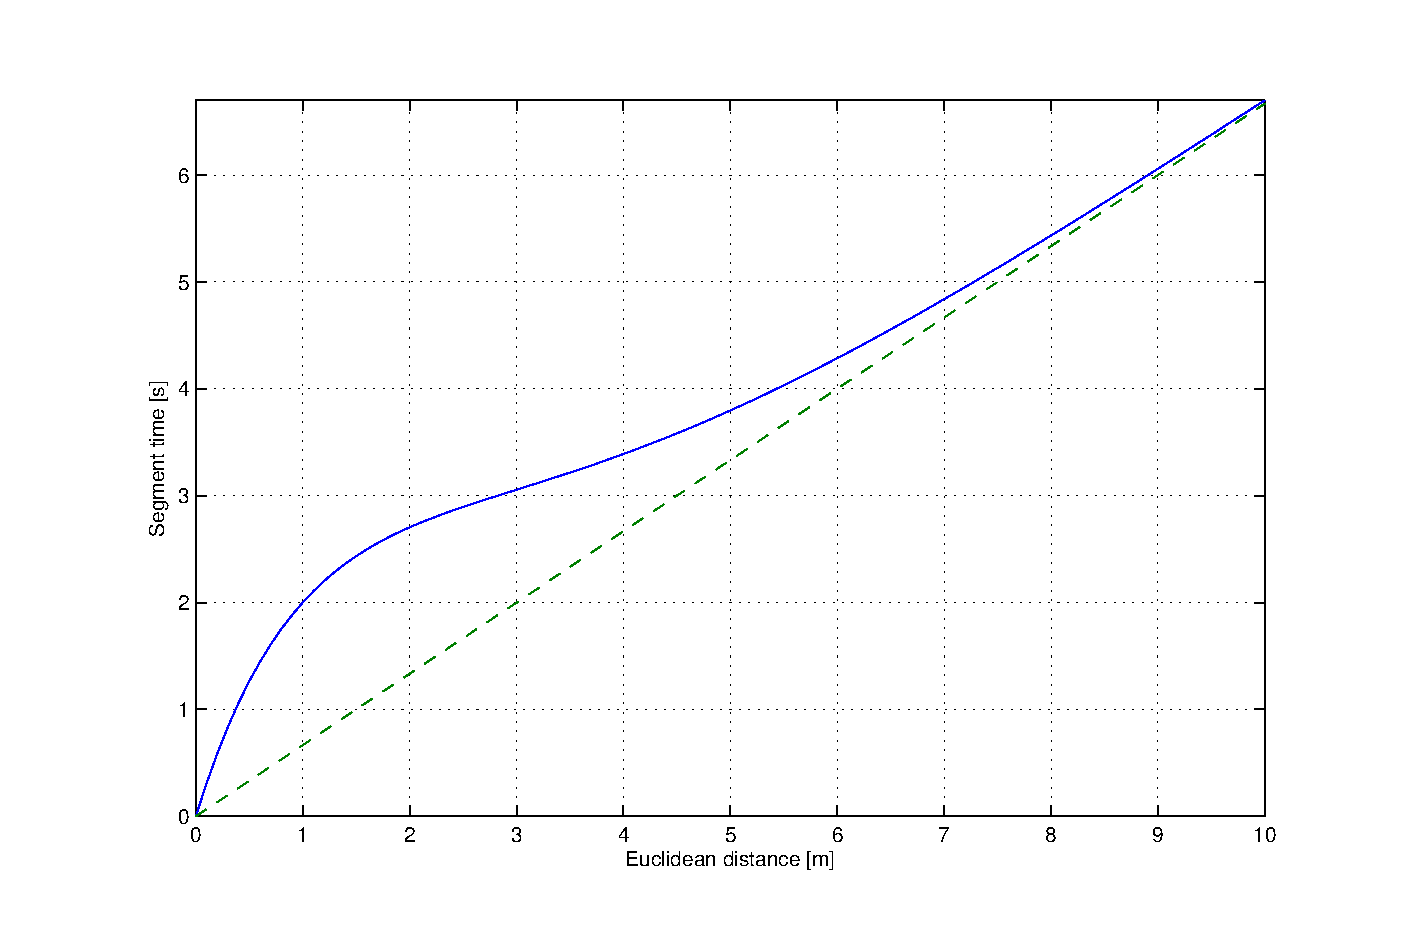
\includegraphics[trim = 20mm 10mm 20mm 10mm,width=1\textwidth]{pics/time_estimation.eps}
   \caption{The segment time $T$ depends on the Euclidean distance $d_{norm}$ of a segment as well as on the max. velocity $v_{max}$ and the max. acceleration $a_{max}$. For short segments the acceleration time is incorporated.}
   \label{pic:timeEstimation}
\end{figure}

Once the segment times are calculated, the initial snap minimized solution can be computed according to equation \ref{equ:dpstar}. The initial solution for a 3 dimensional problem with 2 segments is depict in figure \ref{pic:initialSolution}. The start of the trajectory is the origin of the Cartesian coordinate system (0/0/0). For both, start and goal state, the velocity, the acceleration, the jerk and the snap are fixed and set to zero. For all the other sampling points (vertices) the derivatives are unspecified. The Cartesian coordinates of the sampling points are chosen manually and are listed in the following table: 

\begin{table}[H] 
\begin{center}
    \begin{tabular}{ | l | c | c | c |}
    \hline
    Waypoint & x-coordinate & y-coordinate & z-coordinate\\ \hline
    Start-Vertex & 0 & 0 & 0 \\ \hline
    Vertex 1 & 1 & 2 & 5\\ \hline
    Goal-Vertex & 3 & 4 & 6\\
    \hline
    \end{tabular}
    \caption{3 manually chosen  vertices}
    \label{tab:vertices}
\end{center}
\end{table}


The initial solution depicted in figure \ref{pic:initialSolution} is divided into 3 plots. Plot a) shows the position (i.e. the Cartesian coordinates) whereby each of the 3 dimensions is depicted as a single graph. The Cartesian coordinates from the above-noted table are depicted as circles. 
Plot b) shows the velocity of the individual direction as a solid graph. Additional, the velocity in the three-dimensional space (i.e. the Euclidean norm of the velocity vector) is depicted as a dashed graph.
Plot c) depicts the acceleration in the individual directions (solid) and the acceleration in the three-dimensional space (dashed). Furthermore the limitation for velocity and acceleration ($v_{max} = 3 \frac{m}{s}$ and $a_{max} = 4 \frac{m}{s^2}$ for this problem) are depicted in plot b) resp. c) . The $x$-axis for all the 3 plots is the time. \newpage



\begin{figure}[h]
   \centering
   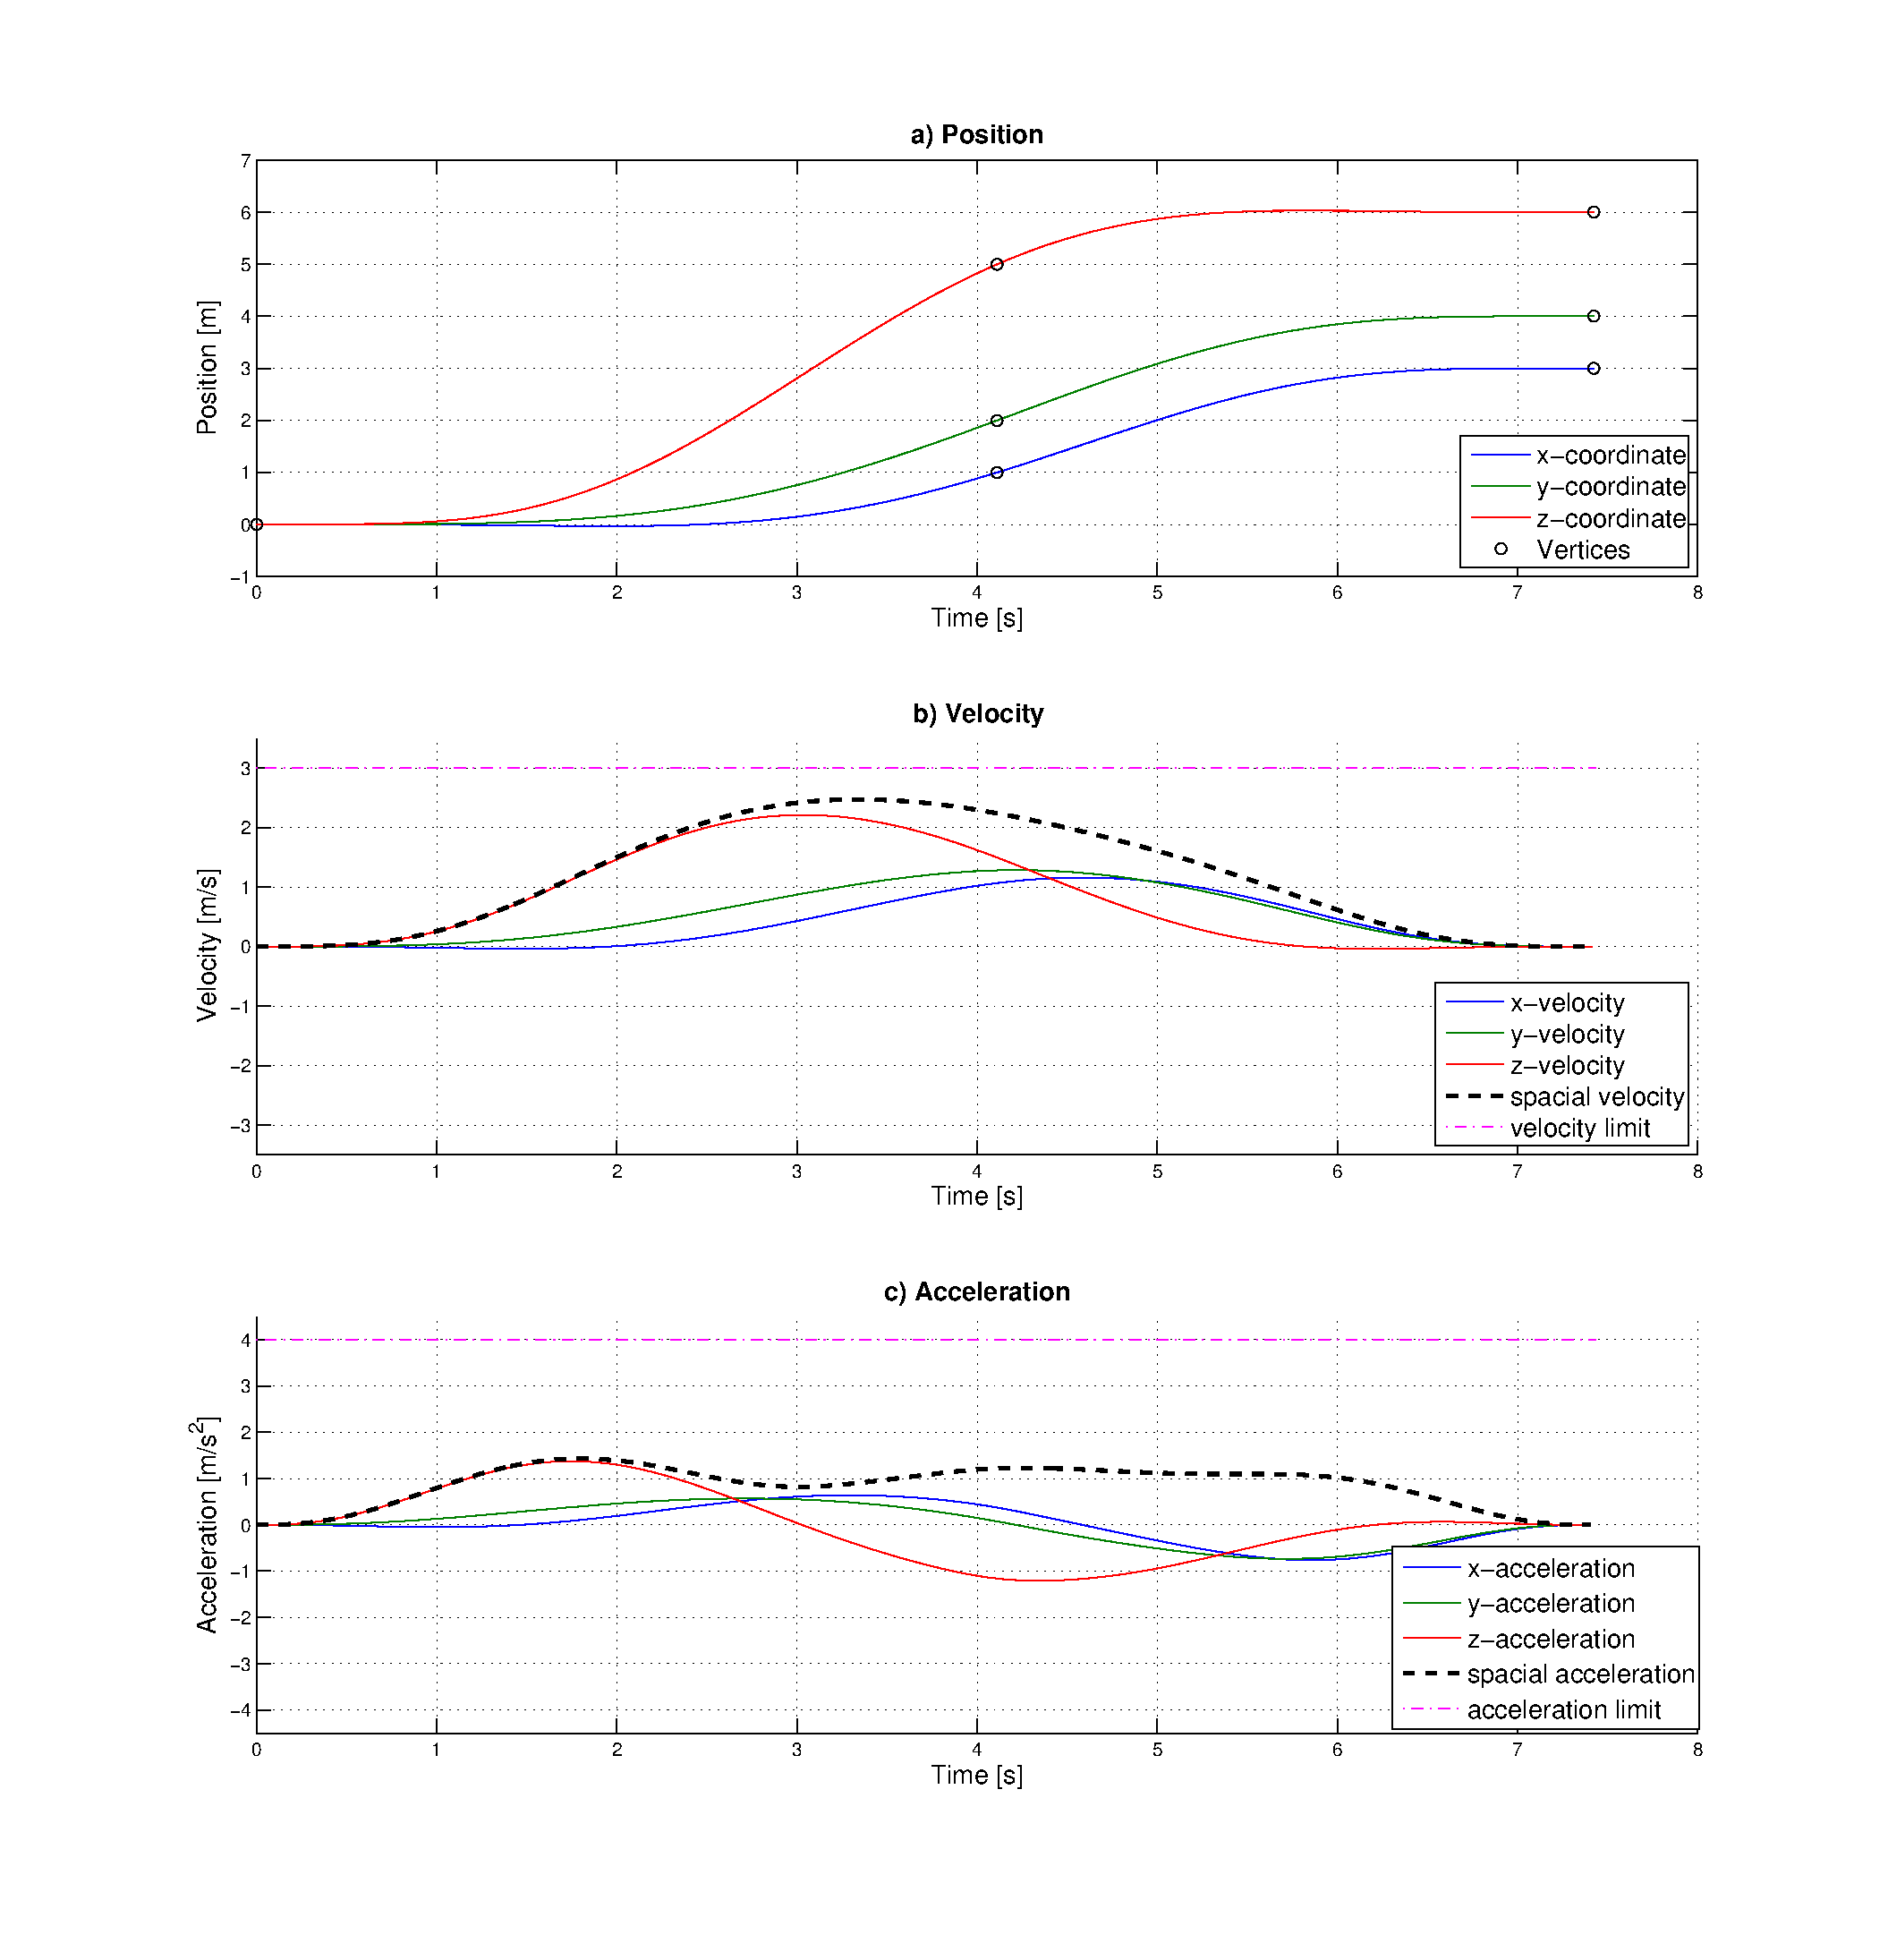
\includegraphics[trim = 35mm 30mm 30mm 15mm,clip,width=1\textwidth]{pics/2SegInit7s43.eps}
   \caption{Initial solution of a trajectory with 2 segments: Plot a) shows the position (i.e. the Cartesian coordinates). Plot b) shows the velocity and plot c) the acceleration. A dashed graph represents the velocity respectively the acceleration in the three-dimensional space.}
   \label{pic:initialSolution}
\end{figure}

As can be seen in plot b) the maximal spacial velocity is less then the user specified maximal velocity $v_{max} = 3\frac{m}{s}$. The same applies to plot c) where the maximal acceleration is far below the user specified maximal acceleration of $a_{max} = 4 \frac{m}{s^2}$. Hence, the trajectory could be more aggressive/faster without violating the limitations. \newline

\subsection{Drawbacks of the Initial Solution}\label{sec:drawbackInitial}


The individual segment times and consequently the total time of the initial trajectory are defined by equation \ref{equ:segmentTime}. Since equation \ref{equ:segmentTime} does not incorporate the circumstances from one segment to an other it is likely to find a better trajectory (i.e. a trajectory with a smaller total cost) with the same total time but a different ratio between the segment time. Moreover there is no possibility to adjust the aggressiveness of the initial solution since the segment times are calculated up front. \newline

Recapitulating, the modification of the individual segment times and therefore the modification of the ratio of the segment times can lead to a better solution. Supplementary, the modification of the individual segment times gives us the opportunity to adjust the aggressiveness of a trajectory.



\section{Time Allocation}\label{sec:penalty}

So fare, only the geometric cost (i. e. the squared snap) was included in the cost function defined in equation \ref{equ:Rxx_cost}. Minimization of the geometric cost ensures a smooth trajectory without abrupt input signal but has no effect on the aggressiveness of a trajectory. Therefore equation \ref{equ:Rxx_cost} has to be extended by the temporal cost (i.e. the sum of the segment times) which results in the total cost $J_{total}$

\begin{equation}
J_{total} =
\begin{bmatrix}
   d_f \\
  d_p
\end{bmatrix}^T
\begin{bmatrix}
   R_{ff} & R_{fp} \\
  R_{pf} & R_{pp}
\end{bmatrix}
\begin{bmatrix}
   d_f \\
  d_p
\end{bmatrix}
+ k_T \cdot \sum_{i=1}^N T_i
\label{equ:total_cost}
\end{equation}

where $k_T$ is a user specified weighting factor and $T_i$ is the segment time of the $i^{th}$ segment. \newline

A hight value for $k_T$ lays weight to the temporal cost and therefore leads to a trajectory with a brief total trajectory time. A small value for $k_T$ on the other hand lays little weight on the temporal cost, meaning the geometric cost gets more important. Since the geometric cost (i.e. the quadratic snap) decreases for long segment times with little changes in jerk, this leads to a trajectory with a long total trajectory time. Thus, the user specified weighting factor $k_T$ enables the adjustment of the aggressiveness of a trajectory. \newline

\subsection{Nonlinear Optimization}\label{sec:nonlinearopt}

The geometric cost function in equation \ref{equ:Rxx_cost} has only the unspecified endpoint derivatives $d_p$ as optimization variables. This optimization problem can be solved analytically as performed in equation \ref{equ:dpstar}. The cost function in equation \ref{equ:total_cost} has the segment times $T_i$ as additional optimization variables. Meaning the segment times $T_i$ are directly represented in the cost function and not only indirectly via the Hessian matrices $Q_{T_i}$. Since the segment times are now optimization variables, the Hessian matrices $Q_{T_i}$ are no longer defined in advance and the problem cannot be solved analytically. Due to that a nonlinear solver is used. In this master thesis NLopt, a open-source library for nonlinear optimization, is applied. The unspecified endpoint derivatives $d_p$ and the segment times $T_i$ of the initial solution are the initial values for the nonlinear solver. Meaning, the initial solution has to be computed in advance to start a nonlinear optimization \newline

To illustrate the nonlinear optimization the trajectory with the same 3 vertices (defined in the table  \ref{tab:vertices}) is reused. In this master thesis position, velocity, acceleration, jerk and snap are fixed for the start and for the goal vertex since we want to start from complete rest and want to end up in standstill. For the vertex in the middle the position is fixed but velocity, acceleration, jerk and snap are unspecified, resulting in the first 4 optimization variables. Since this is a 3 dimensional problem, the number of geometric optimization variables triple to 12. Together with the segment time of the two segments, the problem ends up with a total number of 14 optimization variables. \pagebreak 

%The influence of the number of optimization varibales on the performance is discussed in section: TODO \newline

The result of the nonlinear optimization is depicted in figure \ref{pic:optimizedSolution}. Plot a) depicts the position (i.e. the Cartesian coordinates) whereby each of the 3 dimensions is depicted as a single graph. Plot b) shows the velocity of the individual direction as a solid graph. Additional, the velocity in the three-dimensional space (i.e. the Euclidean norm of the velocity vector) is depicted as a dashed graph. Plot c) depicts the acceleration in the individual directions (solid) and the acceleration in the three-dimensional space (dashed). Furthermore the limitation ($v_{max} = 3 \frac{m}{s}$ and $a_{max} = 4 \frac{m}{s^2}$ for this problem) are depicted.
%\vspace*{3\baselineskip}

\begin{figure}[h]
   \centering
   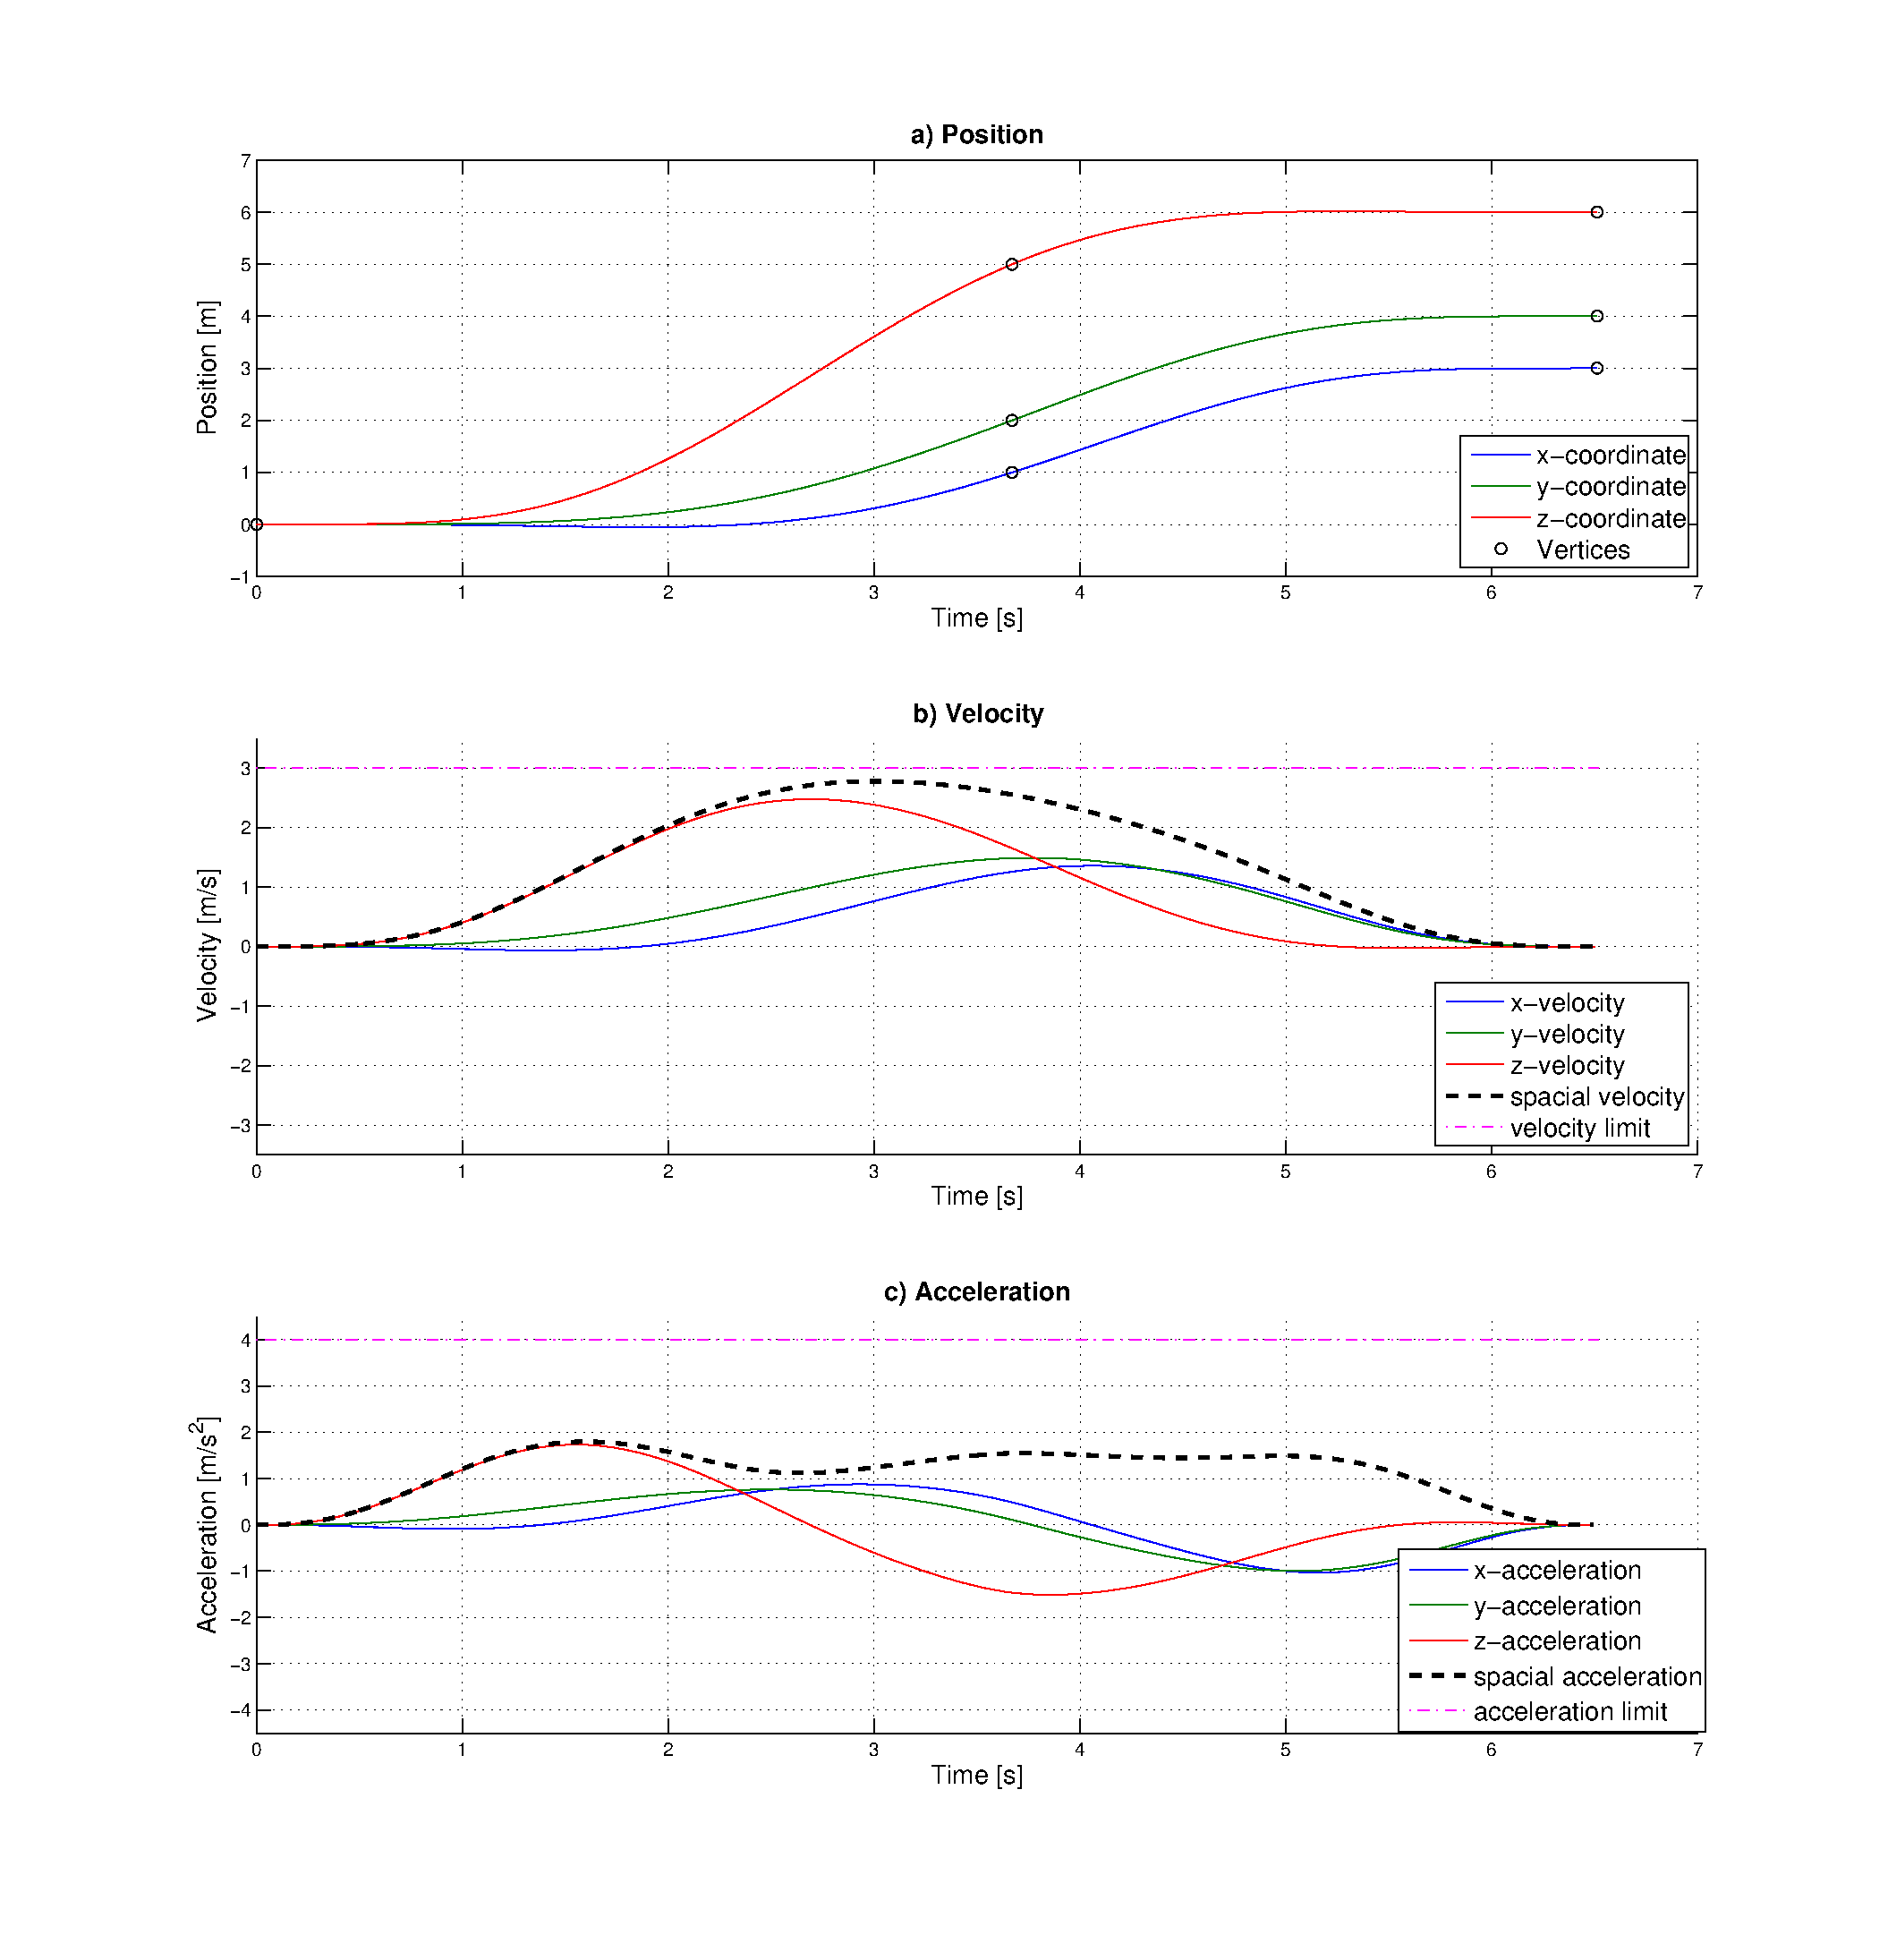
\includegraphics[trim = 35mm 20mm 30mm 8mm,clip,width=1\textwidth]{pics/2SegOpti6s52k100.eps}
   \caption{Optimized solution of a trajectory with 2 segments: Plot a) shows the position (i.e. the Cartesian coordinates). Plot b) shows the velocity and plot c) the acceleration. A dashed graph represents the velocity respectively the acceleration in the three-dimensional space. Weighting factor $k_T$ was set to 100.}
   \label{pic:optimizedSolution}
\end{figure}



As can be seen in figure \ref{pic:optimizedSolution} a) the trajectory passes the same vertices as in figure \ref{pic:initialSolution}. 
In this optimization the user specified weighting factor was set to $k_T = 100$. This rather small value for $k_T$ leads to a trajectory which is neither affected by the limitation on the velocity (the spacial velocity in plot b) is always below the velocity limit) nor by the limitation on acceleration(the spacial acceleration in plot c) is always below the acceleration limit). Nevertheless, the optimized trajectory with a duration of $6.52 s$ is faster then the initial solution with a duration of $7.43 s$.\newline

To get a more aggressive trajectory the value for $k_T$ has to be increased. In figure \ref{pic:optimizedSolution2k190} the optimize trajectory for $k_T = 190$ is depicted. As can be seen in plot b) the limitation on the velocity comes into play, i.e. the spacial velocity is restricted to $v_{max} = 3 \frac{m}{s}$. The duration of the trajectory depicted in figure \ref{pic:optimizedSolution2k190} is $6.01s$. Although the maximal velocity and the maximal acceleration are higher than in figure \ref{pic:optimizedSolution}, the pathway of the spacial velocity and of the spacial acceleration look very similar for $k_T = 100$ and $k_T = 190$.
%\vspace*{3\baselineskip}

\begin{figure}[H]
   \centering
   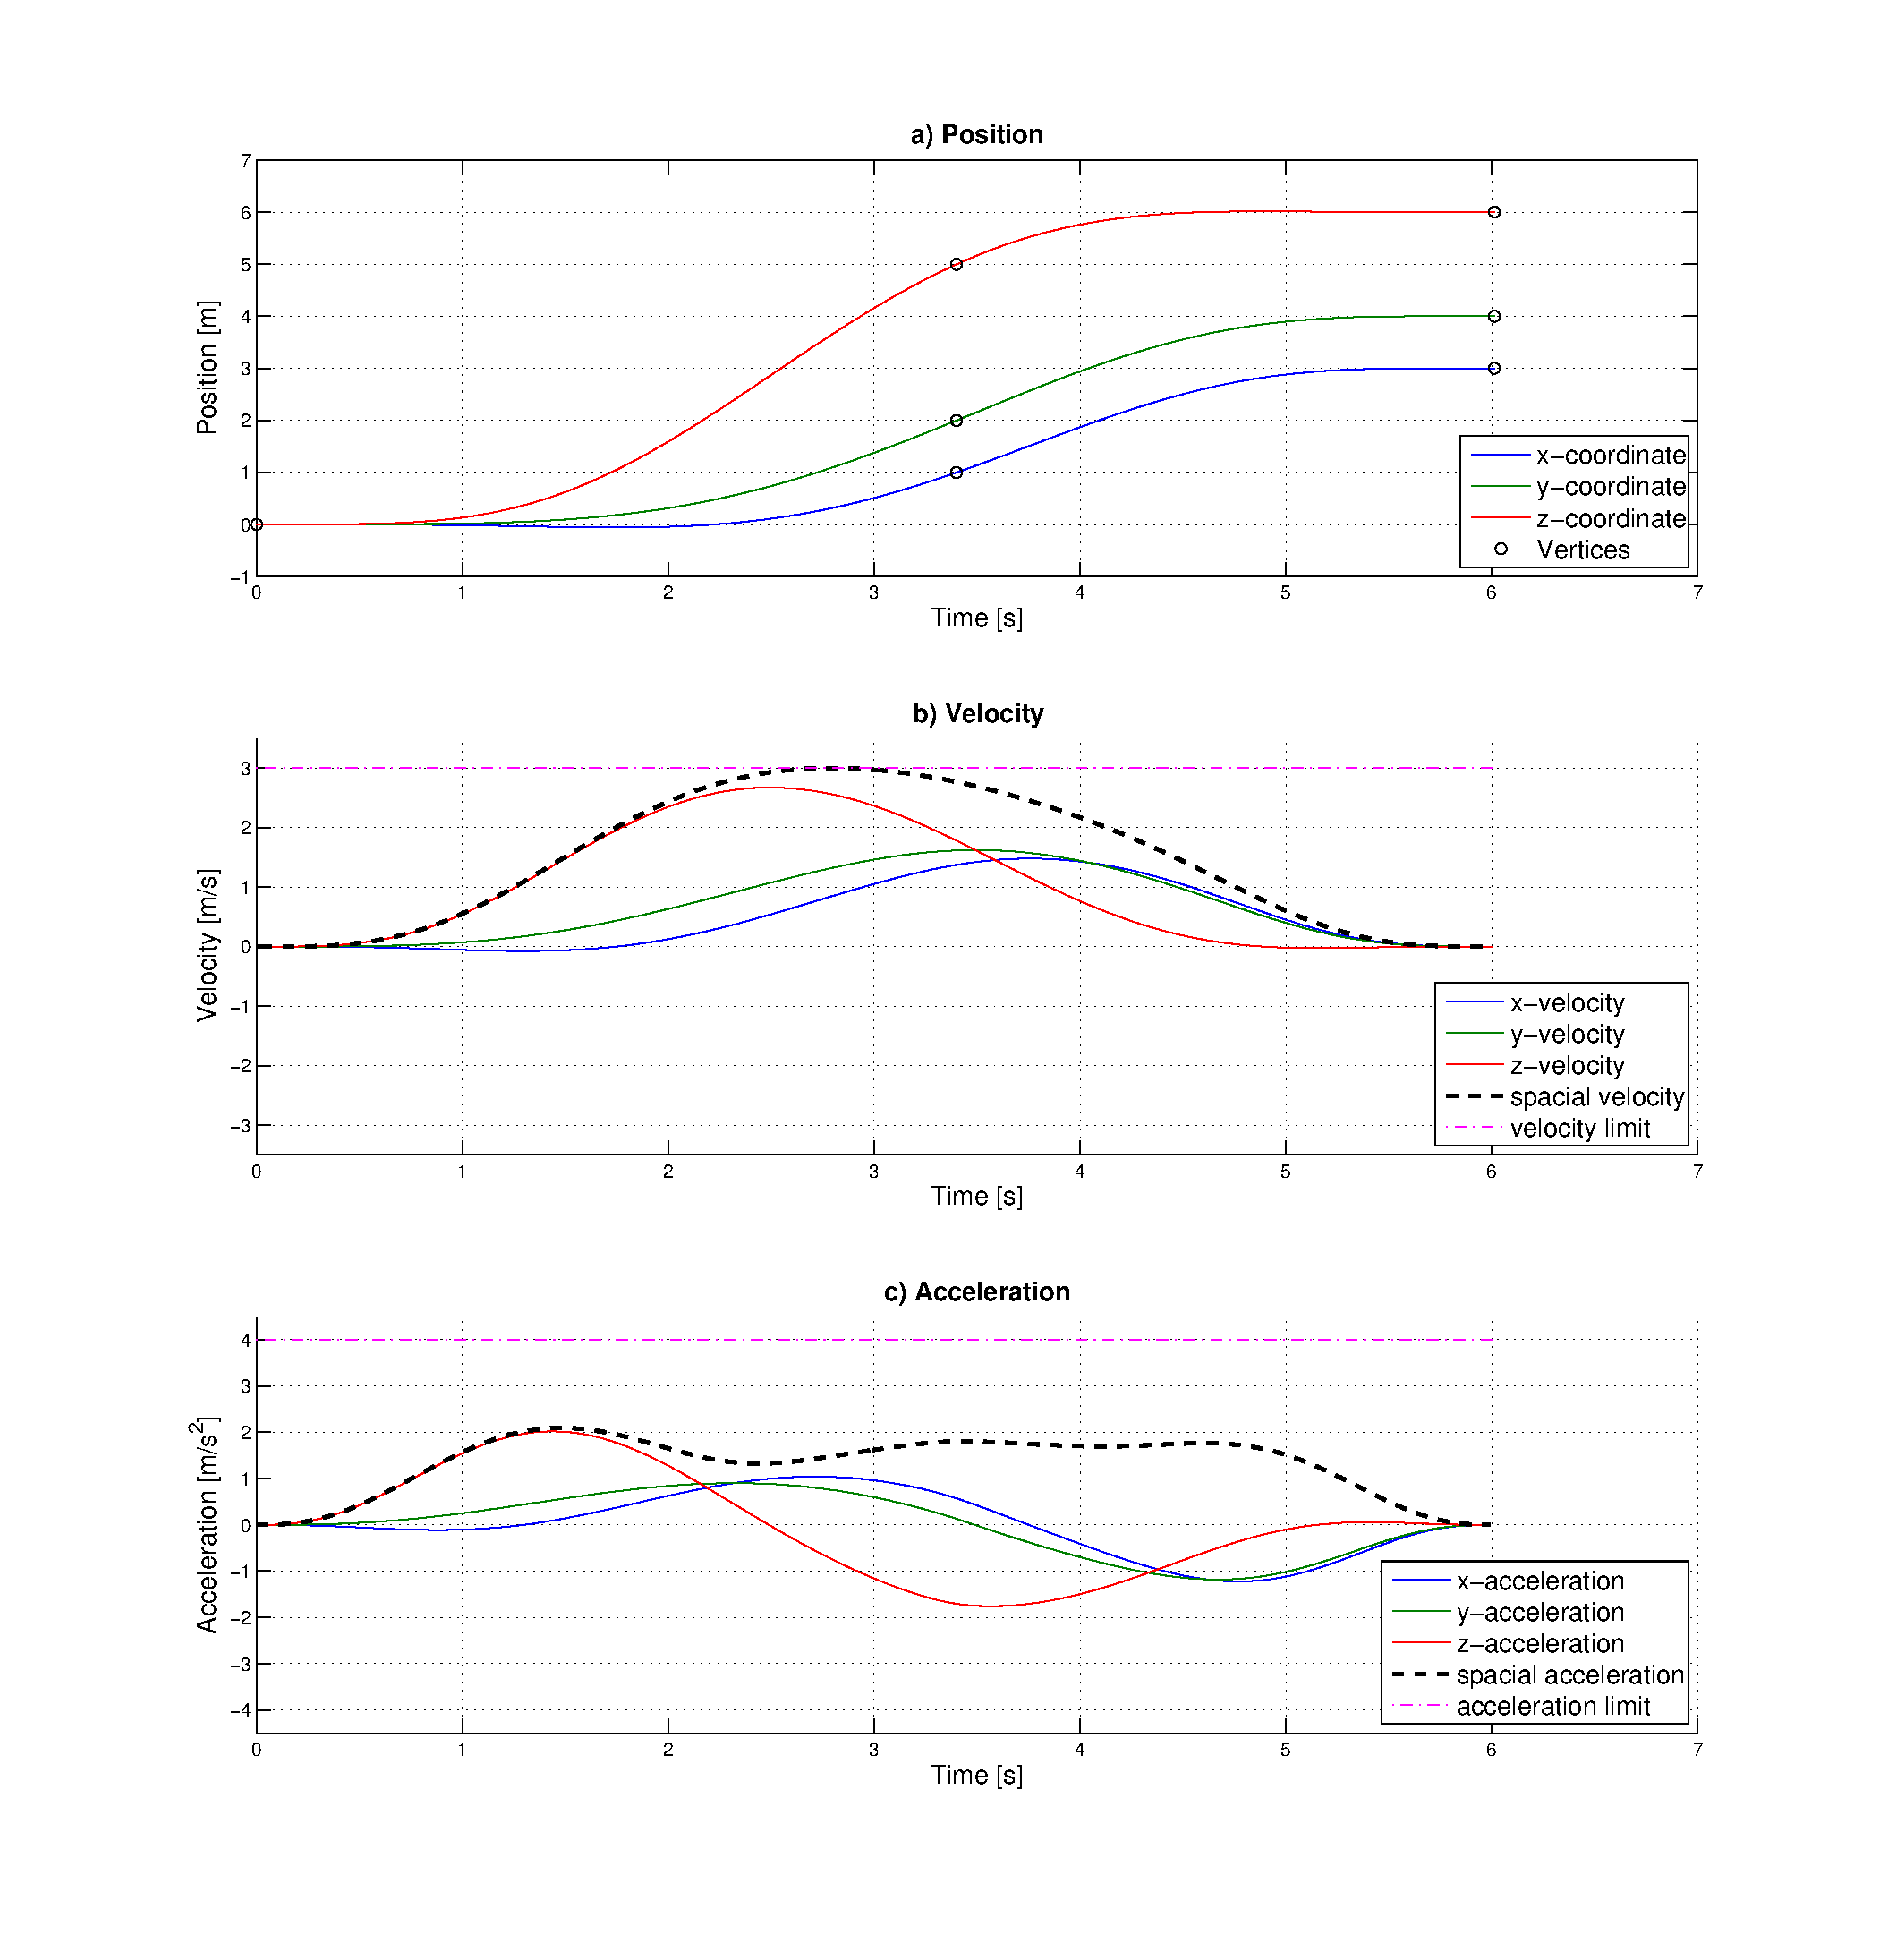
\includegraphics[trim = 35mm 20mm 30mm 15mm,clip,width=1\textwidth]{pics/2SegOpti6s01k190.eps}
   \caption{Optimized solution of a trajectory with 2 segments: Plot a) shows the position (i.e. the Cartesian coordinates). Plot b) shows the velocity and plot c) the acceleration. A dashed graph represents the velocity respectively the acceleration in the three-dimensional space. Weighting factor $k_T$ was set to 190.}
   \label{pic:optimizedSolution2k190}
\end{figure}


In a next step the value for $k_T$ is increased even more and set to $k_T = 2000$. The resulting trajectory is depicted in figure \ref{pic:optimizedSolution2k2000}. The duration of this aggressive trajectory is $5.16s$. The pathway of the spacial velocity looks now different than in the previous figures. The spacial velocity not only touches the velocity limit but stays at the limit for circa one second.
%\vspace*{3.2\baselineskip}

\begin{figure}[H]
   \centering
   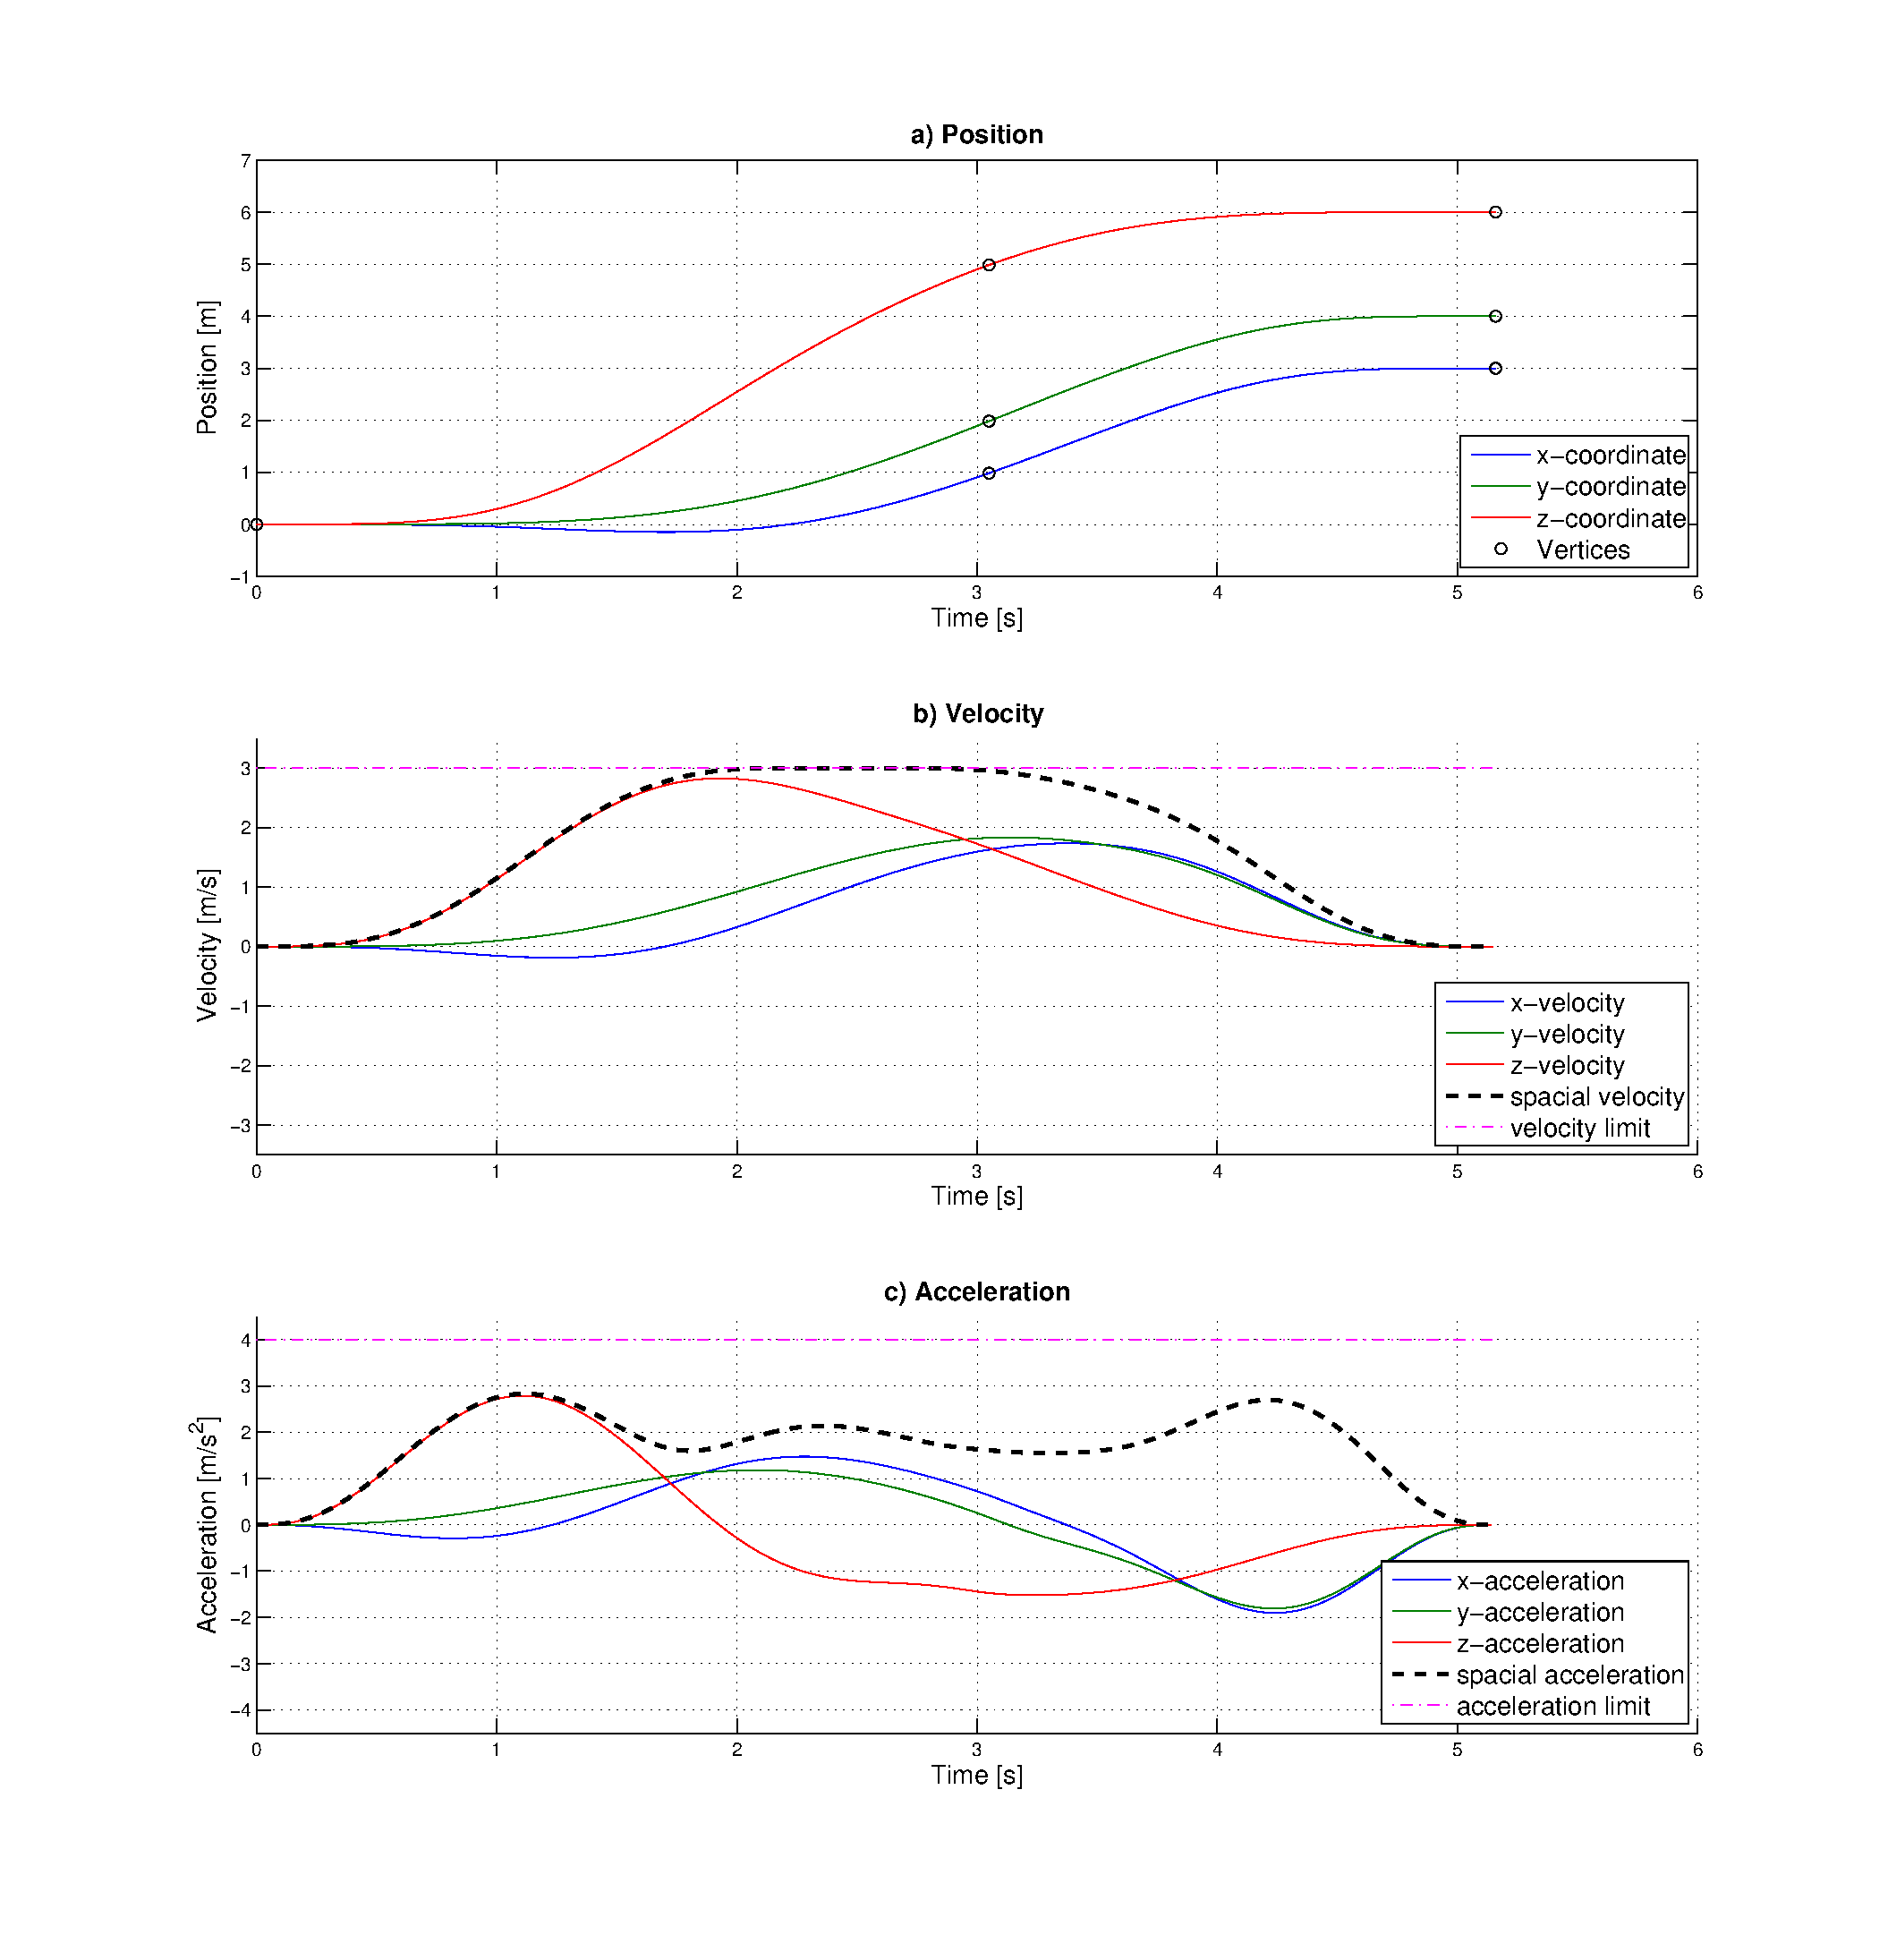
\includegraphics[trim = 35mm 30mm 30mm 15mm,clip,width=1\textwidth]{pics/2SegOpti5s16k2000.eps}
   \caption{Optimized solution of a trajectory with 2 segments: Plot a) shows the position (i.e. the Cartesian coordinates). Plot b) shows the velocity and plot c) the acceleration. A dashed graph represents the velocity respectively the acceleration in the three-dimensional space. Weighting factor $k_T$ was set to 2000.}
   \label{pic:optimizedSolution2k2000}
\end{figure}


Although figure \ref{pic:optimizedSolution2k2000} depicts a aggressive trajectory the spacial acceleration always remains under the acceleration limit. Of course this depends on the choice of the acceleration limit, i.e. the acceleration limit would get significant if $a_{max}$ is set to less than $3 \frac{m}{s^2}$.
A factor which is independent from the user specified choice of $k_T$ is the pathway of the trajectory. For a trajectory with little curves the acceleration has a smaller influence on the duration than the velocity. Since the coordinates in all 3 dimensions increases permanently this is the case in figure \ref{pic:optimizedSolution2k2000}. \newline



To depict the features of a trajectory with more curves an other set of vertices is chosen:

\begin{table}[H] 
\begin{center}
    \begin{tabular}{ | l | c | c | c |}
    \hline
    Waypoint & x-coordinate & y-coordinate & z-coordinate\\ \hline
    Start-Vertex & 0 & 0 & 0 \\ \hline
    Vertex 1 & 5 & 1 & -2\\ \hline
   Vertex 2 & 3 & -2 & 1\\ \hline
   Vertex 3 & -1 & 2 & 3\\ \hline
    Goal-Vertex & 1 & -1 & -2\\
    \hline
    \end{tabular}
\caption{5 manually chosen  vertices}
    \label{tab:5vertices}
\end{center}
\end{table}


The initial solution with 4 segments passing through  the above-noted vertices is depicted in figure \ref{pic:optimizedSolution4init}. 
%\vspace*{4\baselineskip}

\begin{figure}[H]
   \centering
   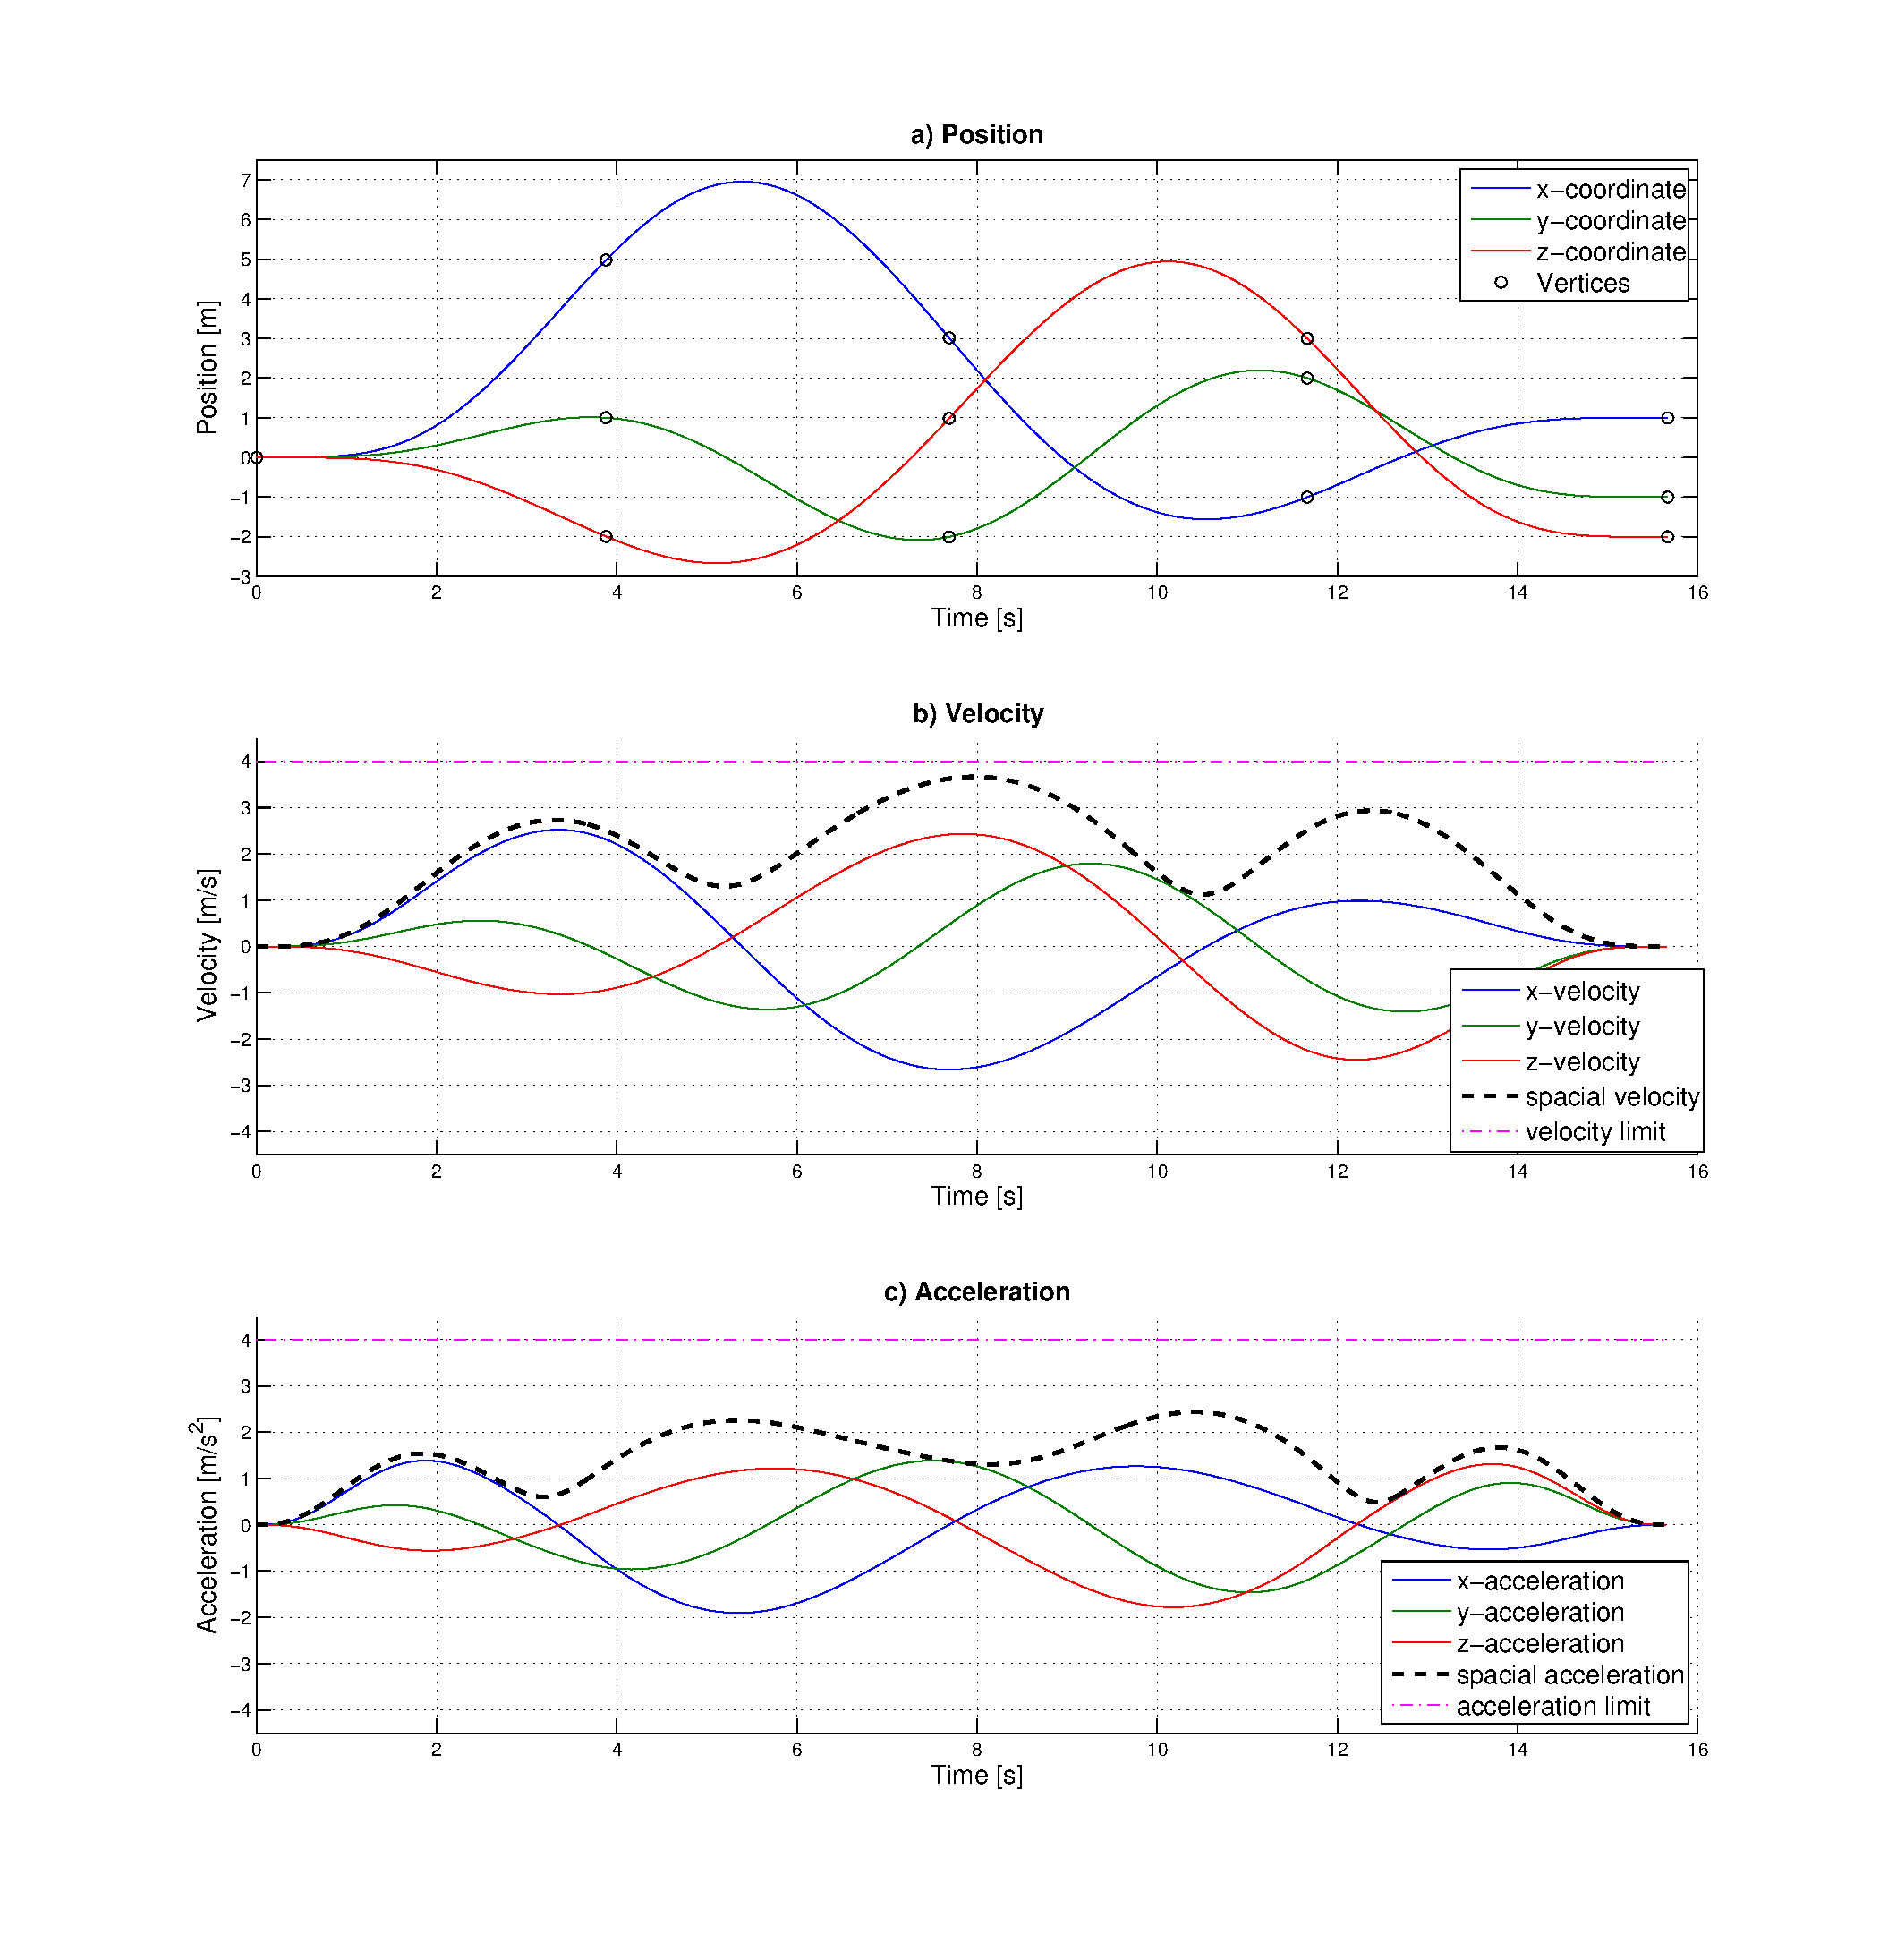
\includegraphics[trim = 35mm 30mm 30mm 15mm,clip,width=1\textwidth]{pics/4SegInit15s67.eps}
   \caption{Initial solution of a trajectory with 4 segments: A dashed graph represents the velocity respectively the acceleration in the three-dimensional space.}
   \label{pic:optimizedSolution4init}
\end{figure}
\newpage

The initial solution is required to define the initial values of the nonlinear optimization.
As can be seen in plot b) and plot c) neither the limitation on the velocity nor the limitation on the acceleration are violated.

%\begin{figure}[h]
%   \centering
%   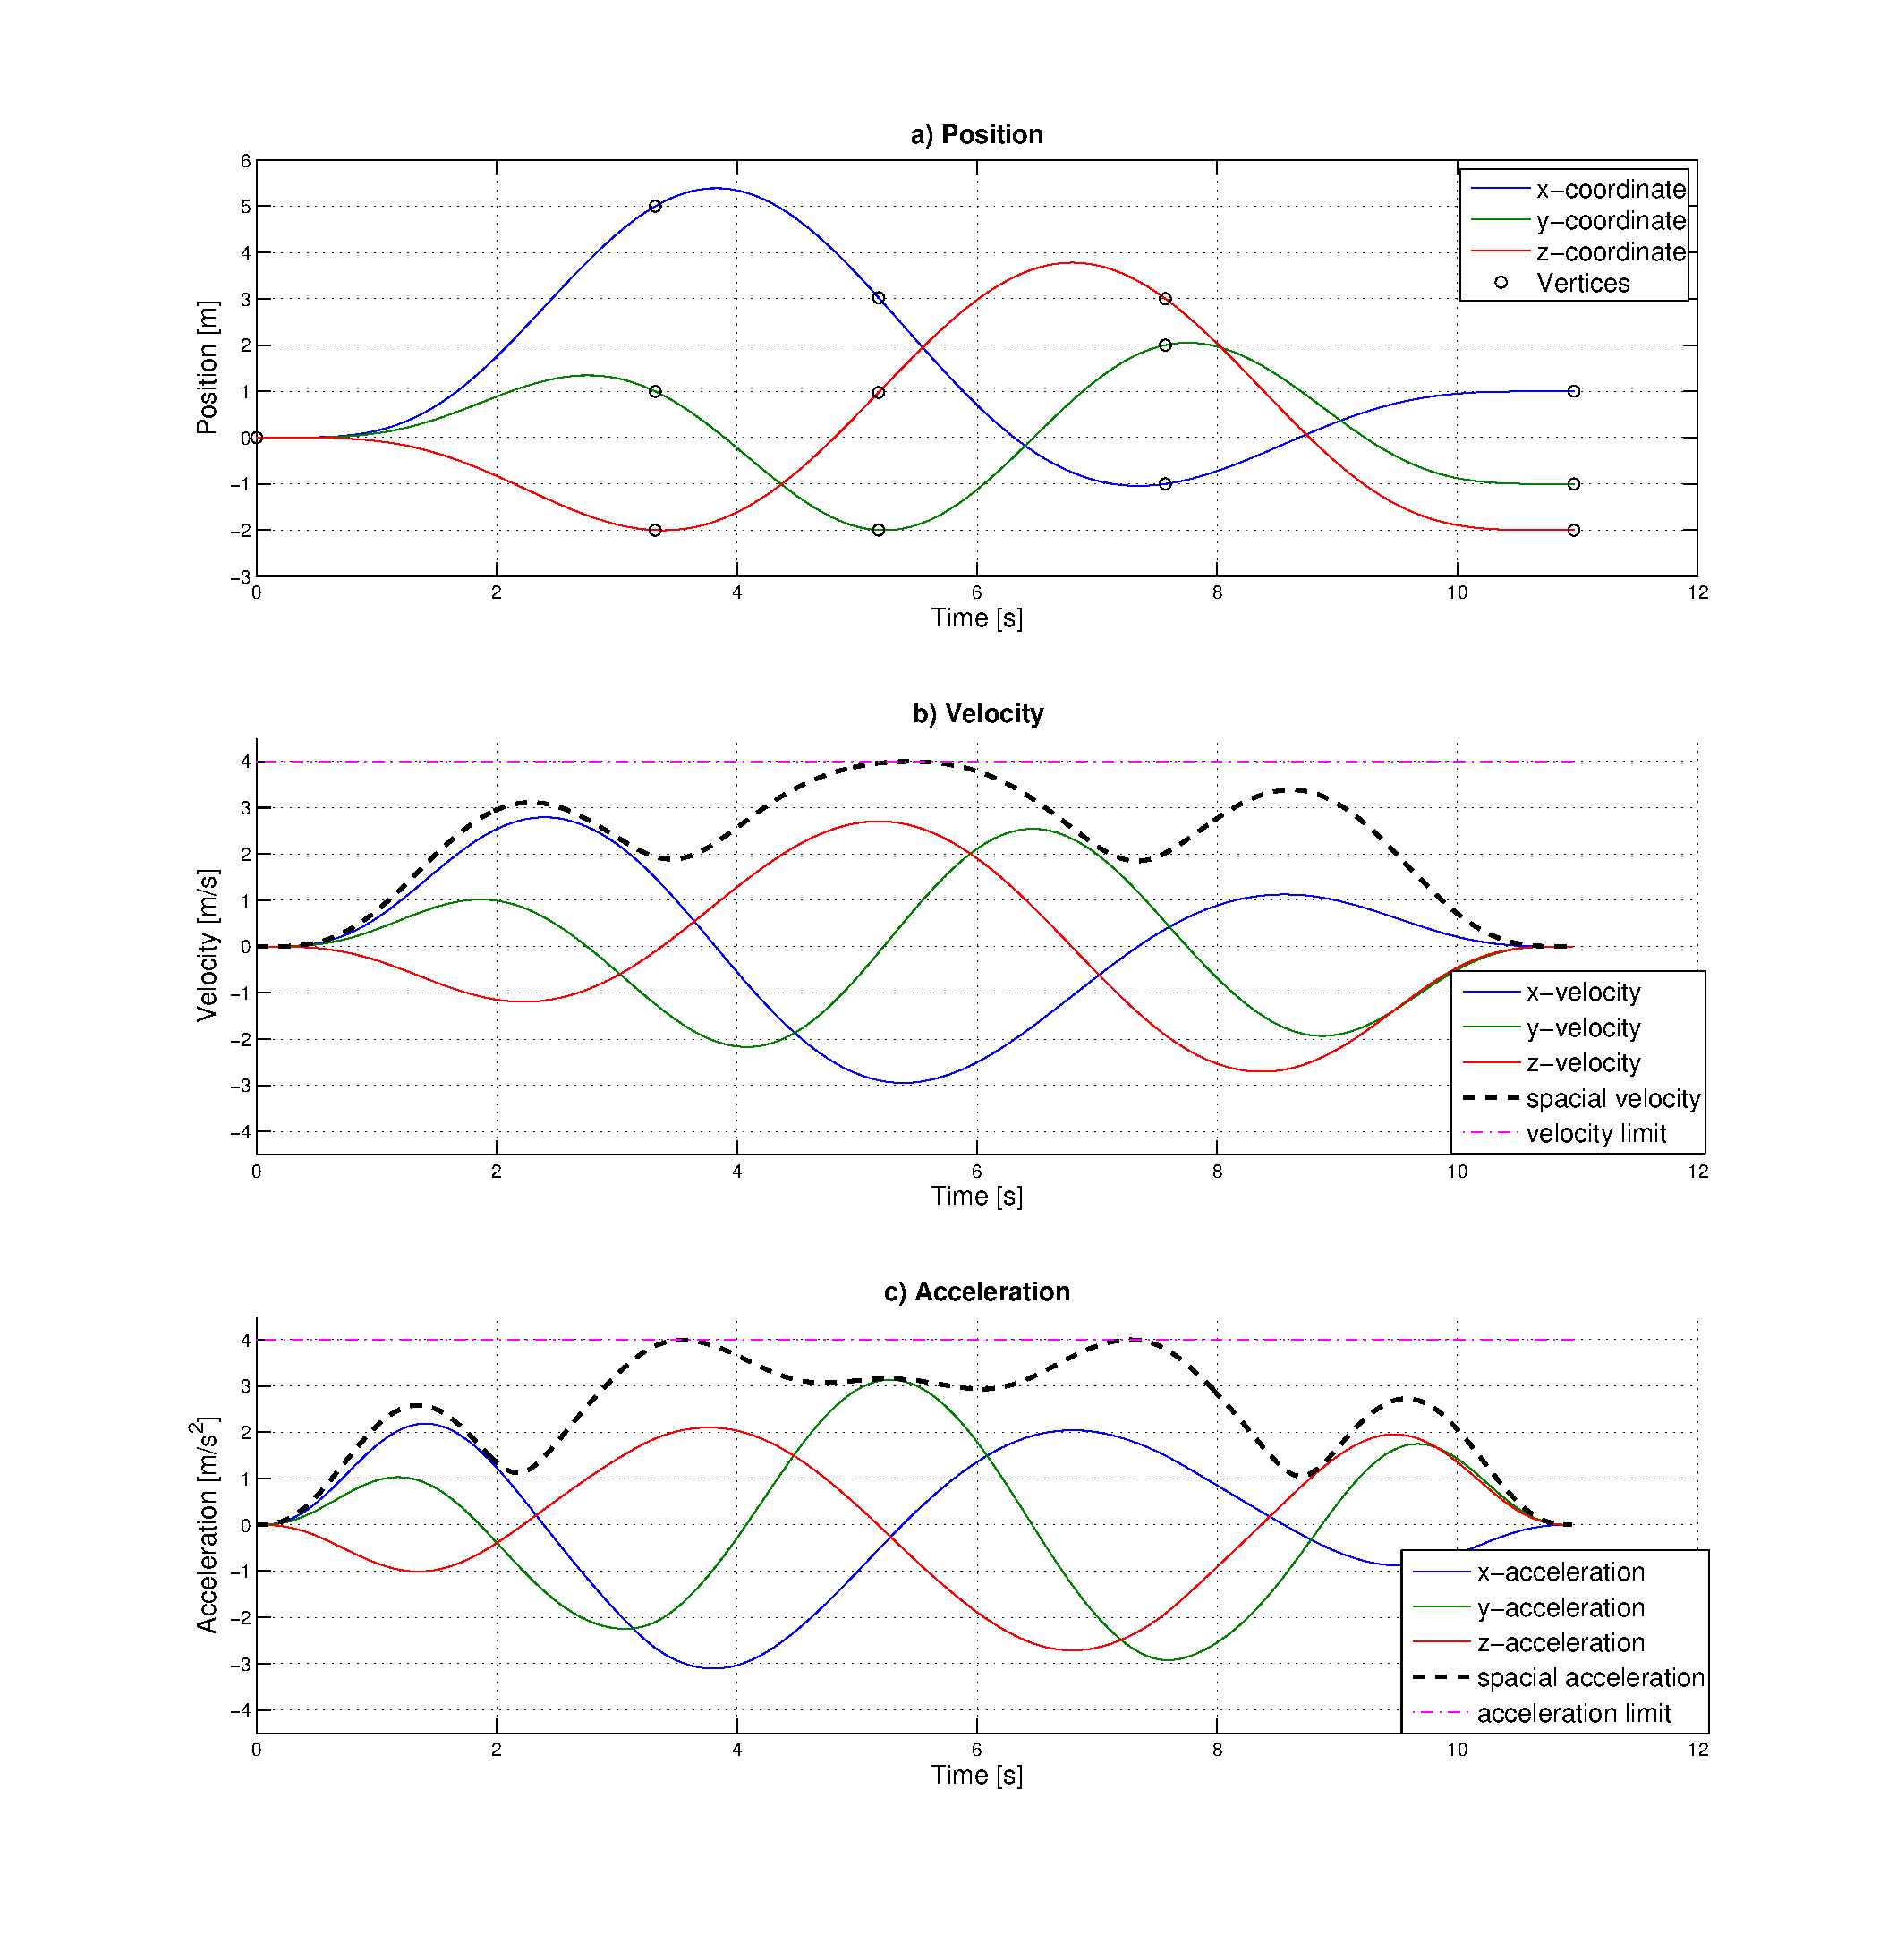
\includegraphics[trim = 35mm 20mm 30mm 35mm,width=1\textwidth]{pics/4SegOpti10s97k400.eps}
%   \caption{...................................................................................... ..... ............. . . . . ...................... ......... .........}
%\end{figure}


Using the unspecified enpoint derivatives $d_P$ and the segment times $T_i$ of the initial solution as initial values for the optimization variables the nonlinear optimization was performed with a weighting factor of $k_T = 2000$. The optimized trajectory is depicted in figure \ref{pic:optimizedSolution4optik2000}. The duration of the optimized trajectory is $10.02s$ whereas the duration of the initial trajectory depicted in figure \ref{pic:optimizedSolution4init} is $15.67s$.


\begin{figure}[H]
   \centering
   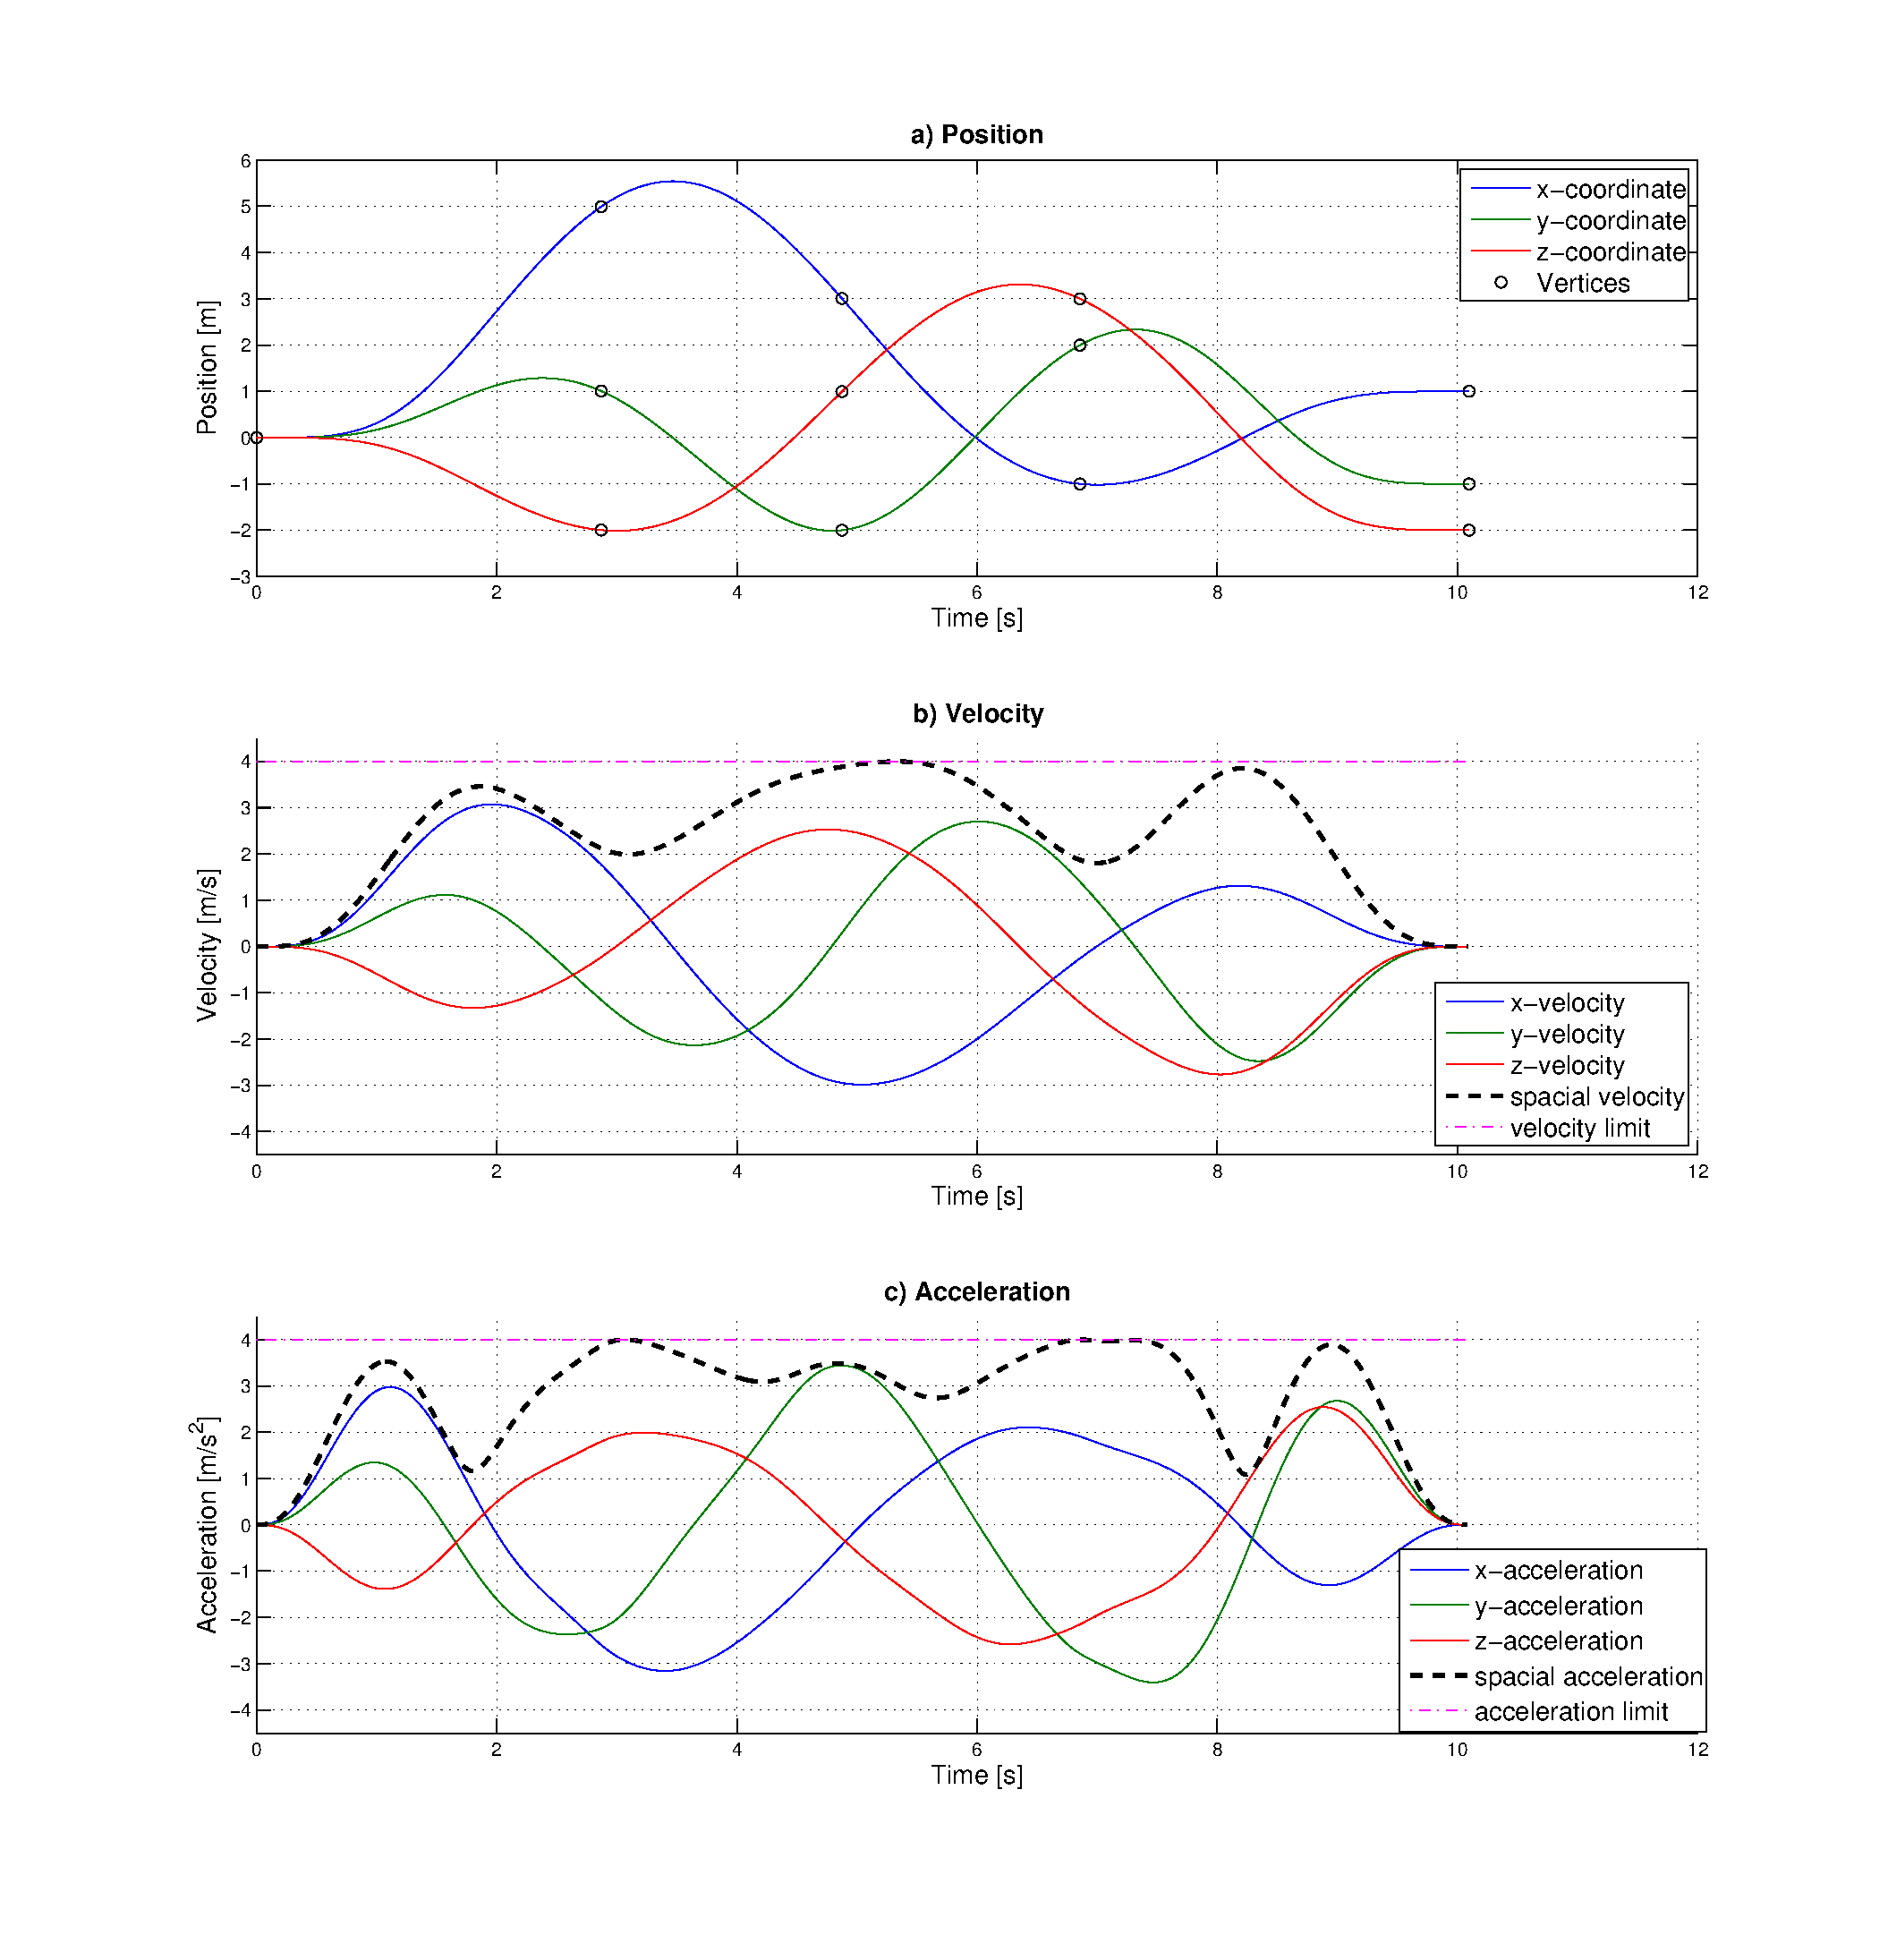
\includegraphics[trim = 35mm 30mm 30mm 15mm,clip,width=1\textwidth]{pics/4SegOpti10s01k2000.eps}
   \caption{Optimized solution of a trajectory with 4 segments: A dashed graph represents the velocity respectively the acceleration in the three-dimensional space. Weighting factor $k_T$ was set to 2000.}
   \label{pic:optimizedSolution4optik2000} 
\end{figure}

In contrast to the aggressive trajectory depicted in figure \ref{pic:optimizedSolution2k2000}, the acceleration limit has a impact on the optimized curvy trajectory in figure \ref{pic:optimizedSolution4optik2000}. As can be seen in plot c) the spacial acceleration touches the acceleration limit repeatedly and even stays at exact $4 \frac{m}{s^2}$ for some time. 

\section{Pathway of the Trajectory}\label{sec:pathway}

The pathway of a snap minimized trajectory is mainly determined by the ratio of the segment times and not by the segment times themselves or by the total trajectory time. As mention in section \ref{sec:drawbackInitial}, the segment times from the initial solution do not incorporate the circumstances from one segment to an other. Hence, it is likely to find a better trajectory with the same total time but a different ratio between the segment time. The process of optimizing the ratio of the segment times is implicitly performed during the process of nonlinear optimization. In other words, the nonlinear optimization not only changes the total trajectory time according to the weighting factor $k_T$ but also optimizes the ratio of the segment times. \newline
Such a change in the pathway is distinguishable between the initial trajectory in figure \ref{pic:optimizedSolution4init} a) and the optimized trajectory in figure \ref{pic:optimizedSolution4optik2000} a). The easiest notable difference is the peak of the $x$ graph with a peak value of 6.95 in the initial trajectory and a peak value of 5.58 in the optimized trajectory. Nevertheless, the changes in the pathway are more presentable in a 3D plot. 


\begin{figure}[H]
   \centering
   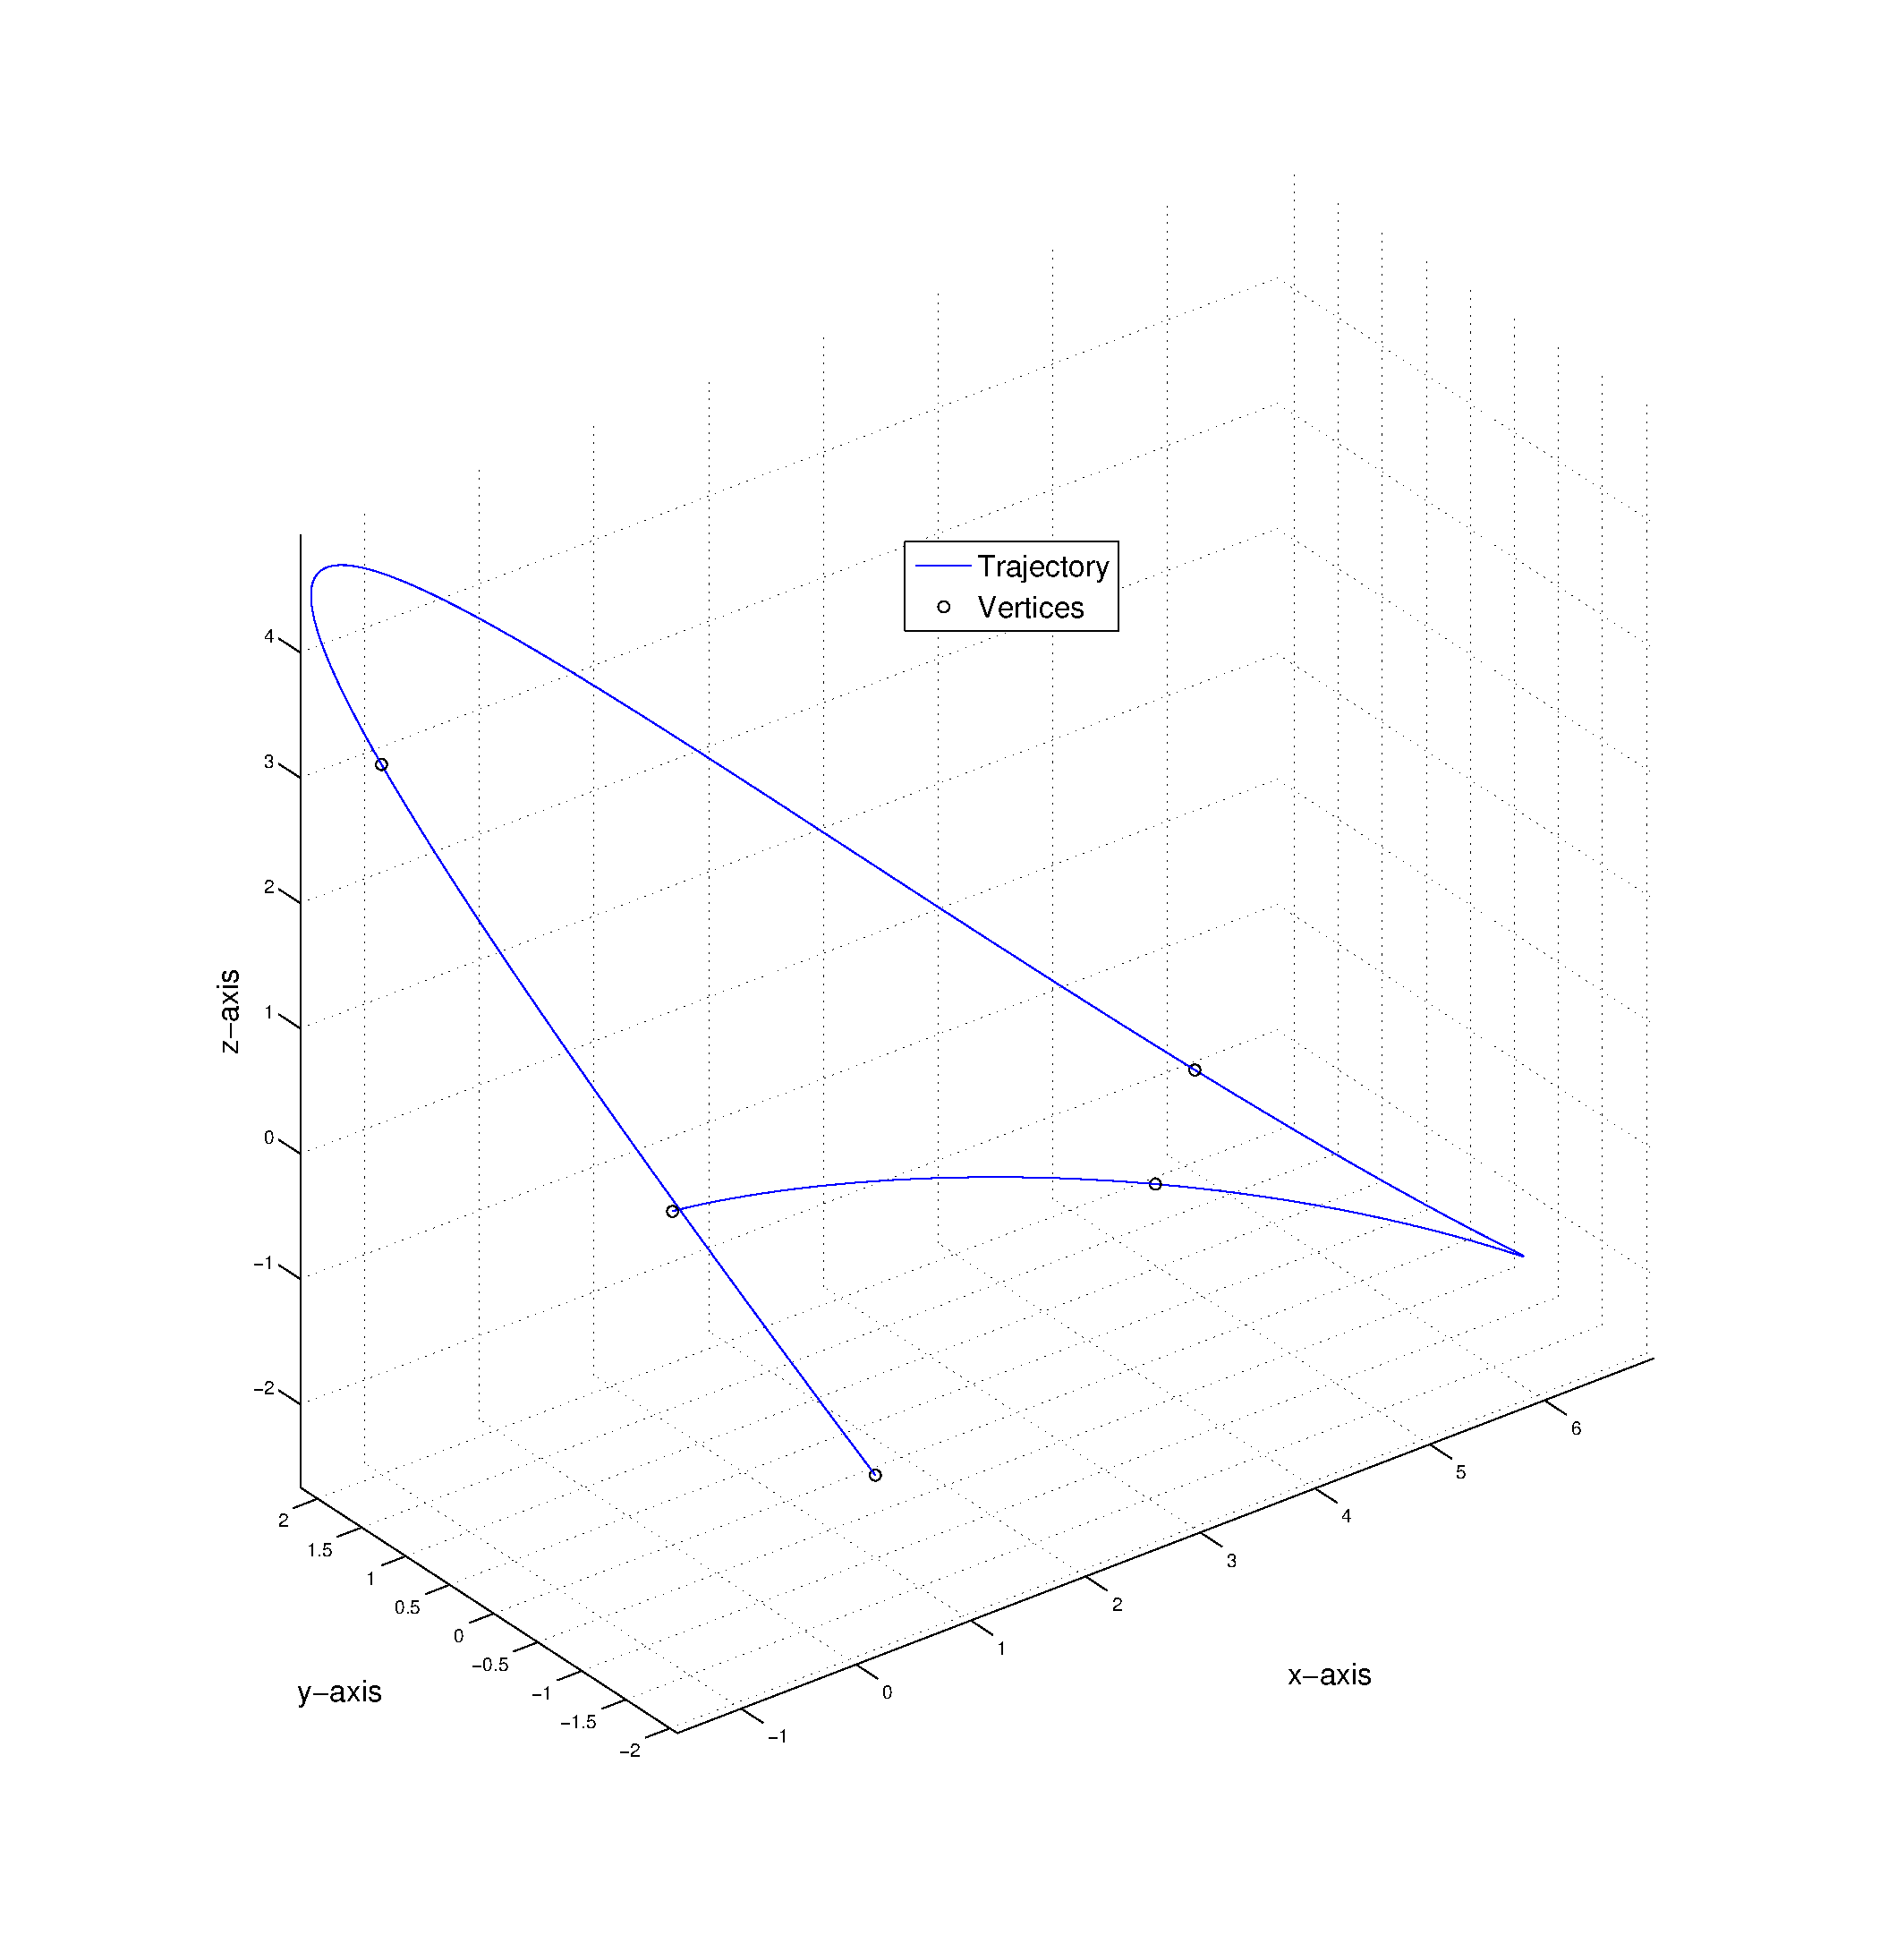
\includegraphics[trim = 36mm 30mm 33mm 30mm,clip,width=1\textwidth]{pics/4SegInitSpace.eps}
   \caption{3D plot of the initial trajectory with 4 segments.The start vertex is located at (0/0/0) and the trajectory proceeds clockwisely.}
   \label{pic:initiSpace} 
\end{figure}


Figure \ref{pic:initiSpace} depicts the initial trajectory (from figure \ref{pic:optimizedSolution4init}) in 3D space. Again, the vertices are marked as circles but now the times is no longer explicit readable. The start vertex is located at (0/0/0) and the trajectory proceeds clockwisely. The second segment (lower right corner) of the initial trajectory in figure \ref{pic:initiSpace} looks very sharp. Such sharp corners, accrued by the suboptimal segment time ratio, are undesirable if the UAV should fly a trajectory dynamically. \newline

The optimization of the ratio of the segment times, which is implicitly performed during the nonlinear optimization, modifies the pathway of the trajectory which gets smoother, i.e. no sharp corner exist in the optimized trajectory.\newline 
Figure \ref{pic:optiSpace} depicts the optimized trajectory (from figure \ref{pic:optimizedSolution4optik2000}) in 3D space. Especially the second segment of the optimized trajectory is now more suitable for a dynamic flight. But also the pathway in the region of the 4. vertex (in the upper left corner) is enhanced. The initial trajectory mad a detour before passing the 4 Vertex. This detour, accrued by the suboptimal segment time ratio, is vanished in the optimized trajectory.



\begin{figure}[H]
   \centering
   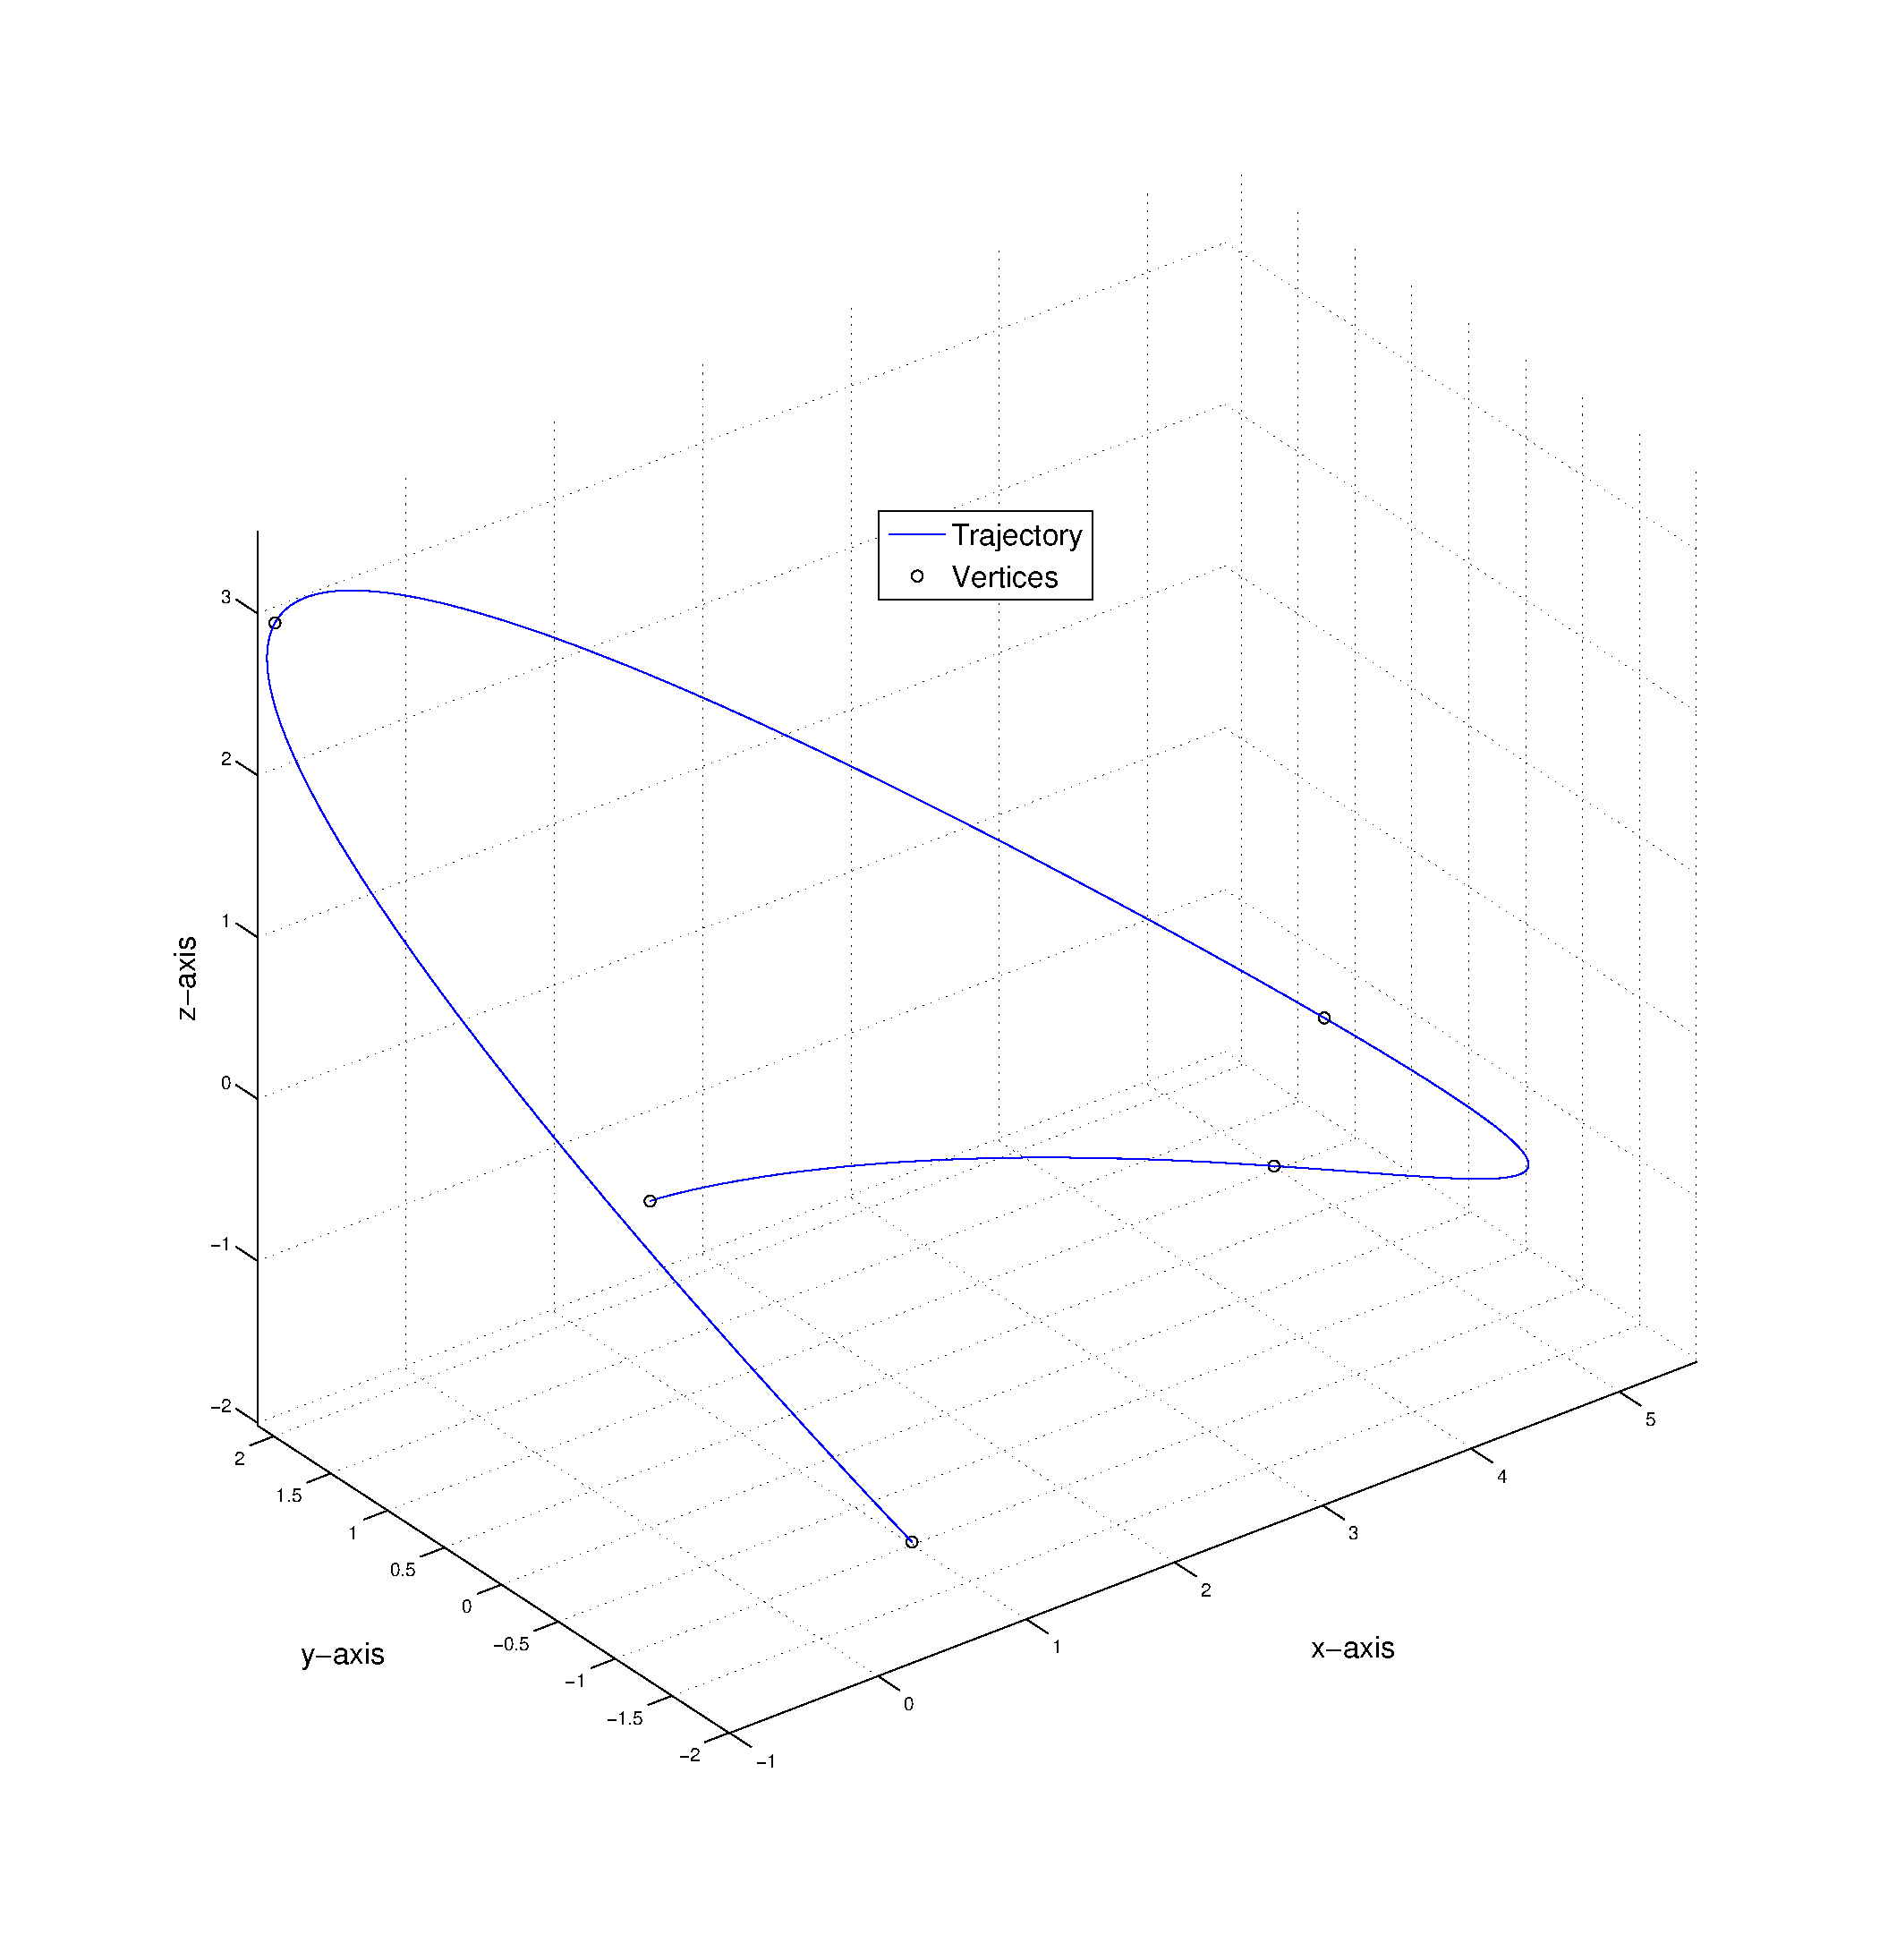
\includegraphics[trim = 36mm 30mm 33mm 30mm,clip,width=1\textwidth]{pics/4SegOptiSpace.eps}
   \caption{3D plot of the optimized trajectory with 4 segments.The start vertex is located at (0/0/0) and the trajectory proceeds clockwisely.}
    \label{pic:optiSpace} 
\end{figure}
\newpage


\section{NLopt}\label{sec:NLopt}

For all the nonlinear optimizations which were performed in the previous sections, NLopt, a open-source library for nonlinear optimization, was applied. The optimization algorithm tries to minimize the cost function every iteration and needs some kind of termination condition in order to know when to stop.\newline
The termination condition of the optimization can be specified by the optimization variables as well as by the total cost. Generally, the termination conditions are formulated relative to the current value(s). For instance, if the relative termination condition for the total cost $J_{rel}$ is set to $0.01$ the optimization ends if the total cost changes less than one percent during an iteration. The relative termination condition for the optimization variables $x_{rel}$ is only fulfilled if all of the optimization variables change less than the threshold in an iteration.
Additionally, an absolute termination condition $x_{abs}$ can be applied to the optimization variables. This termination condition is only needed if one or several optimization variables are close to zero and the relative criteria therefore don't work properly. \newline 
Two additional options are the limitation of the number of optimization iterations and the limitation of the duration of the optimization. All of these termination condition can be set simultaneously and the first condition which is fulfilled stops the optimization.
During the optimization the constraints on velocity and acceleration are checked every iteration. \newline










%Once the segment times are calculated, the initial snap minimized solution can be computed according to equation \ref{equ:dpstar}. The initial solution for a 3 dimensional problem with 4 segments is depict in figure \ref{pic:initialSolution}. The start of the trajectory is the origin of the Cartesian coordinate system (0/0/0). For both, start and goal state, the velocity, the acceleration, the jerk and the snap are fixed and set to zero. For all the other sampling points (vertices) the derivatives are unspecified. The Cartesian coordinates of the sampling points are chosen manually and are listed in the following table: 
%




%\begin{figure}[h]
%   \centering
%   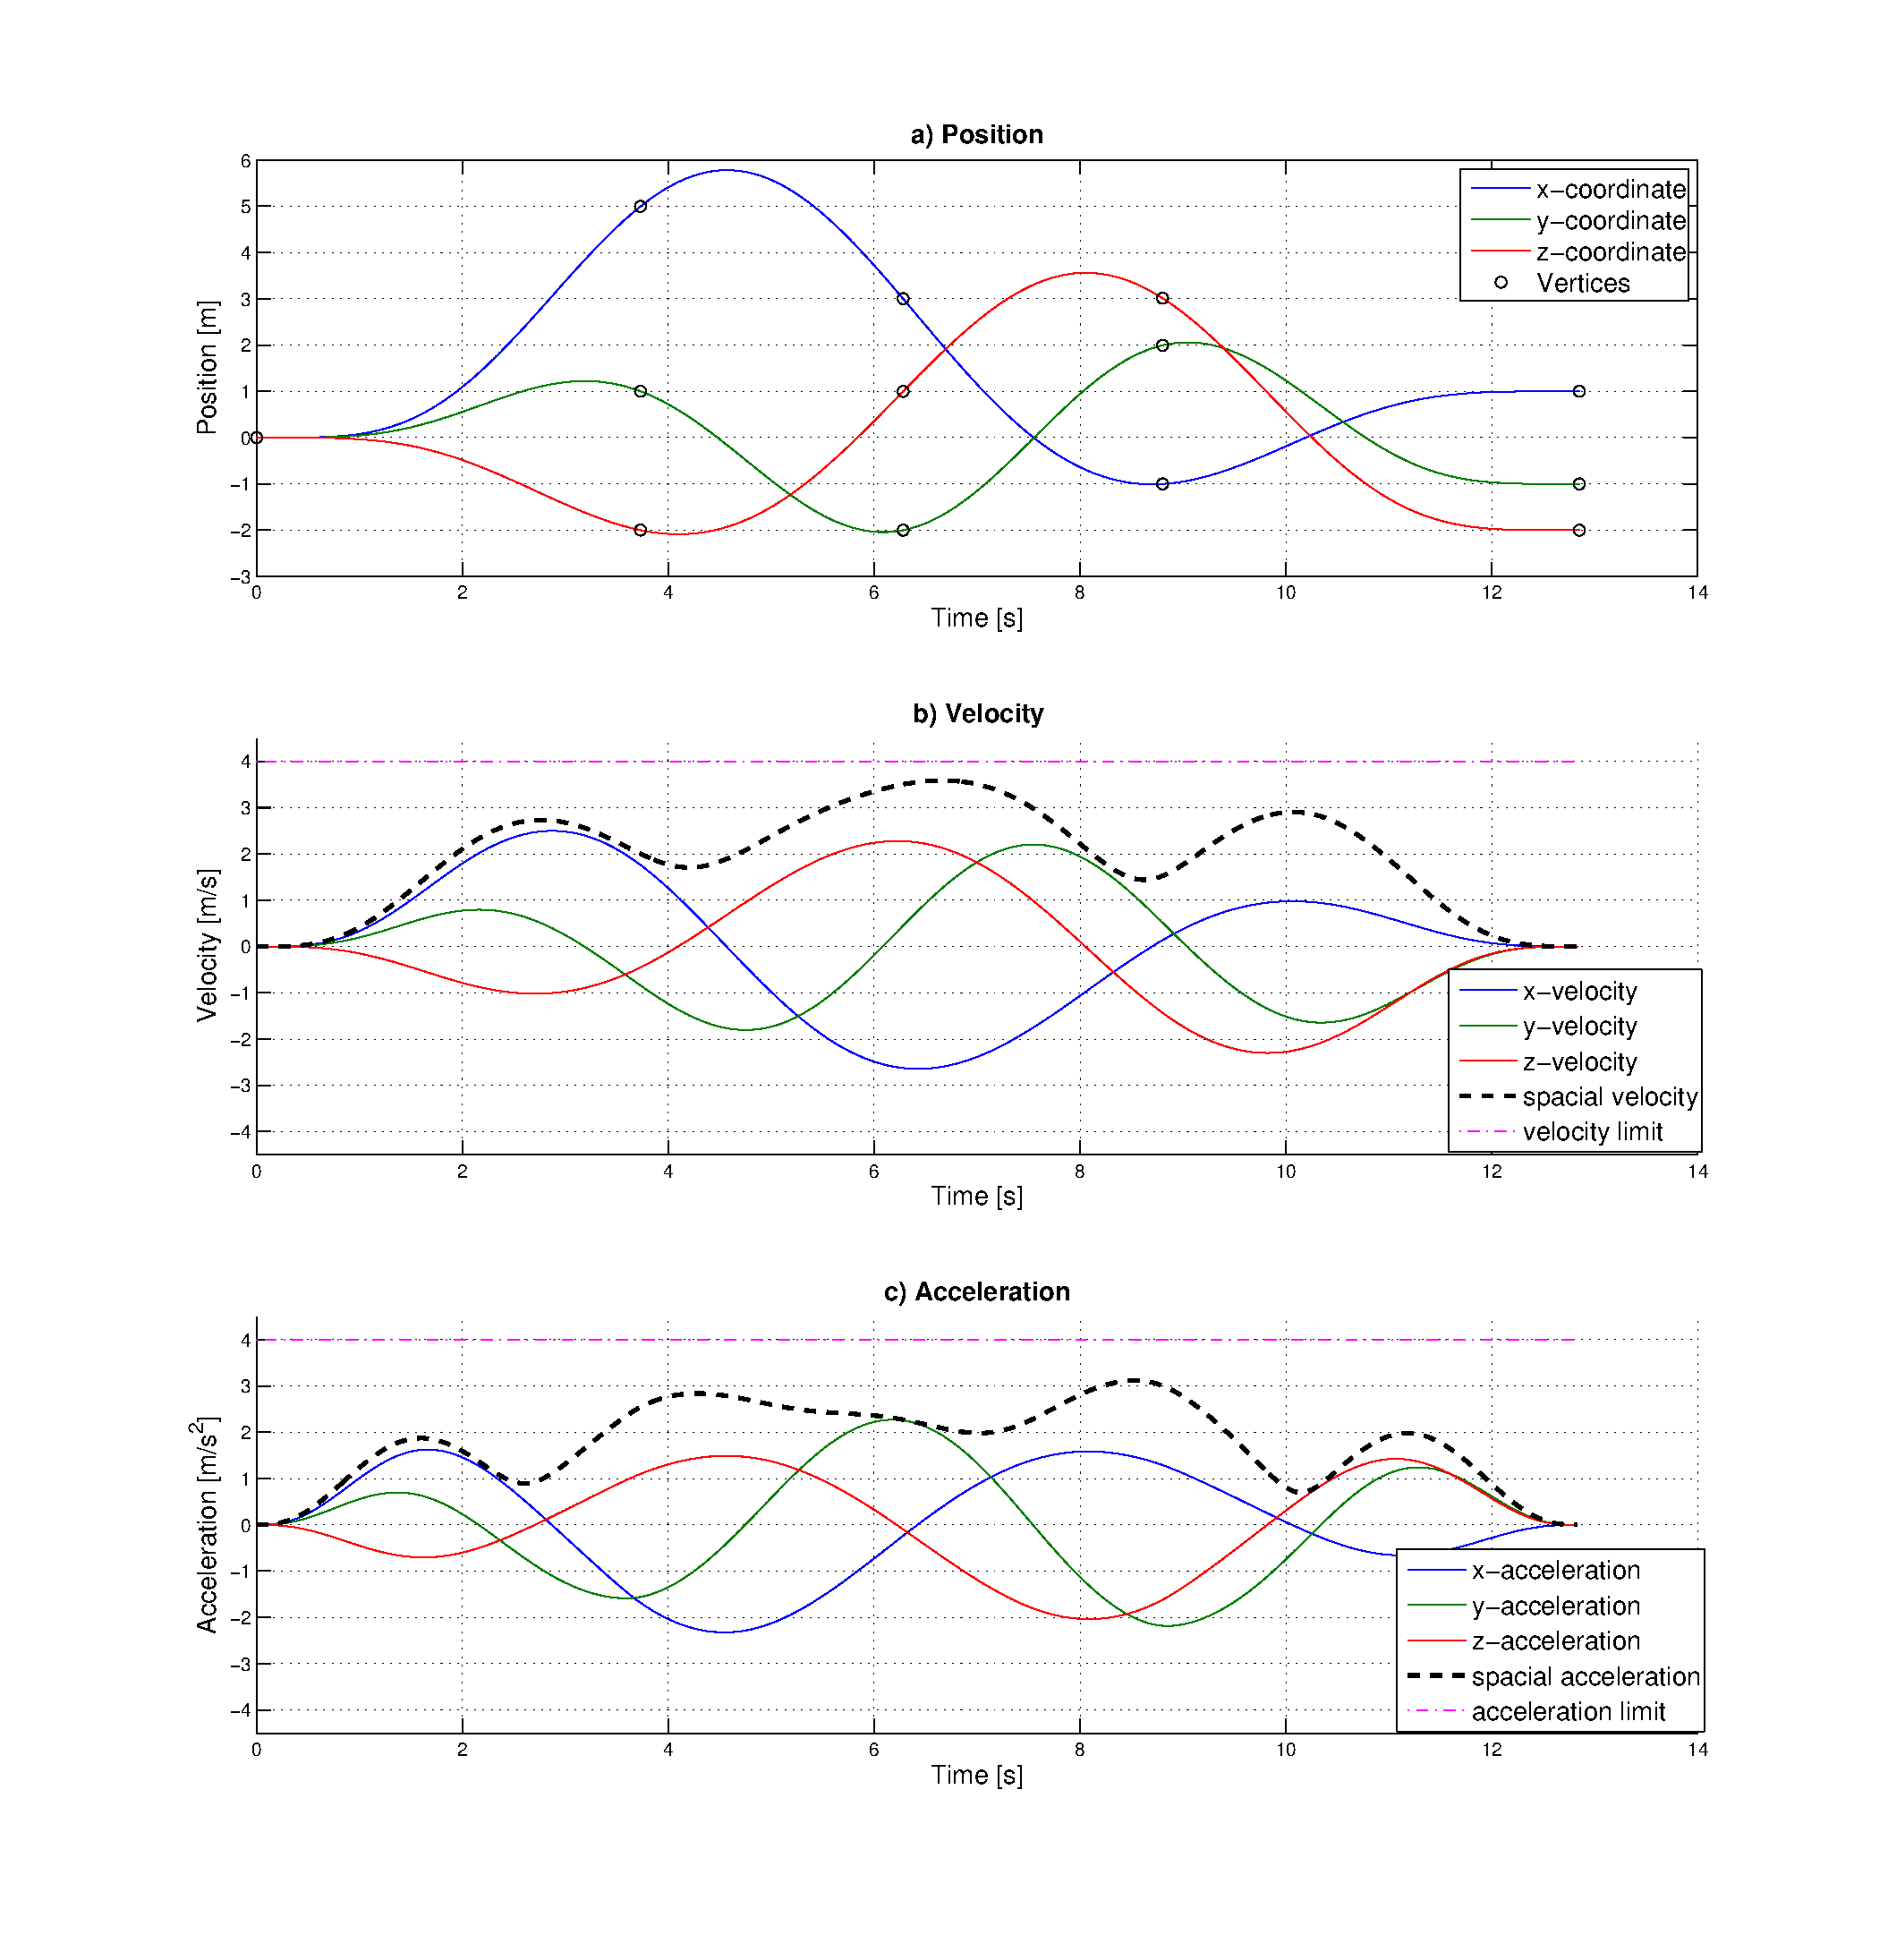
\includegraphics[trim = 35mm 20mm 30mm 35mm,width=1\textwidth]{pics/4SegOpti12s85k100.eps}
%   \caption{...................................................................................... ..... ............. . . . . ...................... ......... .........}
%\end{figure}
%
%
%
%
%





%\texttt{\begin{figure}[h]
%   \centering
%   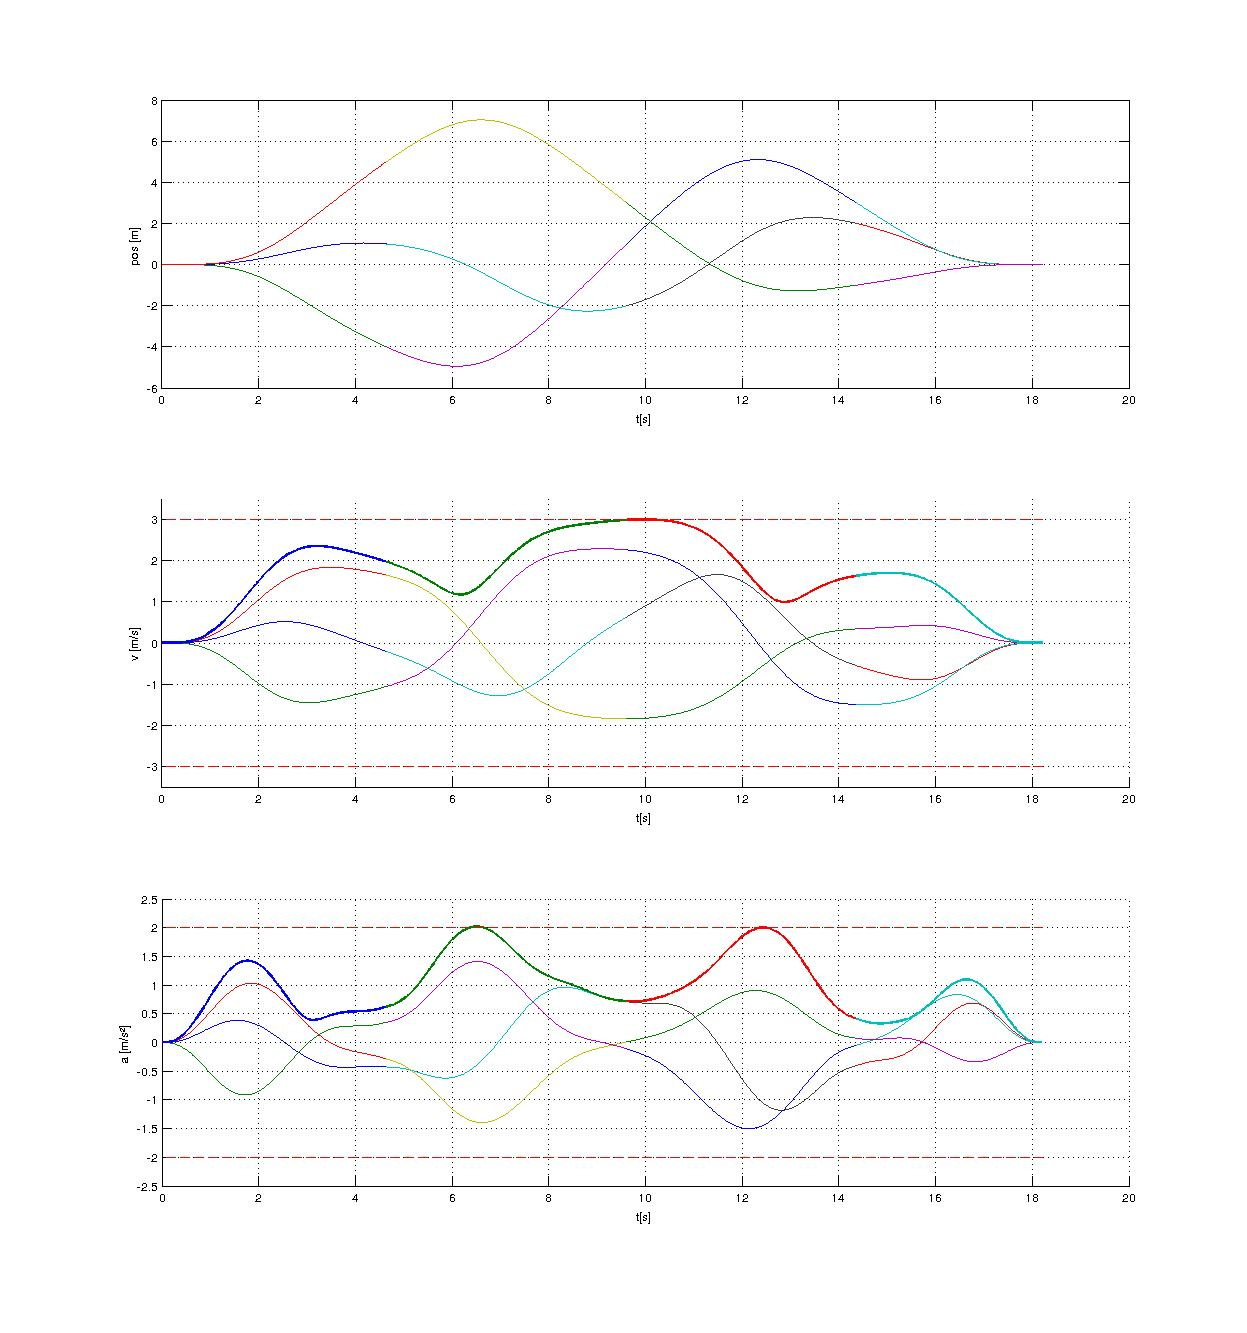
\includegraphics[width=1\textwidth]{pics/optimized.jpg}
%   \caption{Optimized solution of a trajectory with 4 segments: Plot a) shows the position (i.e. the Cartesian coordinates). Plot b) shows the velocity and plot c) the acceleration. A dashed graph represents the velocity respectively the acceleration in the three-dimensional space.}
%   \label{pic:optimizedSolution}
%\end{figure}}





%\begin{figure}[h]
%   \centering
%   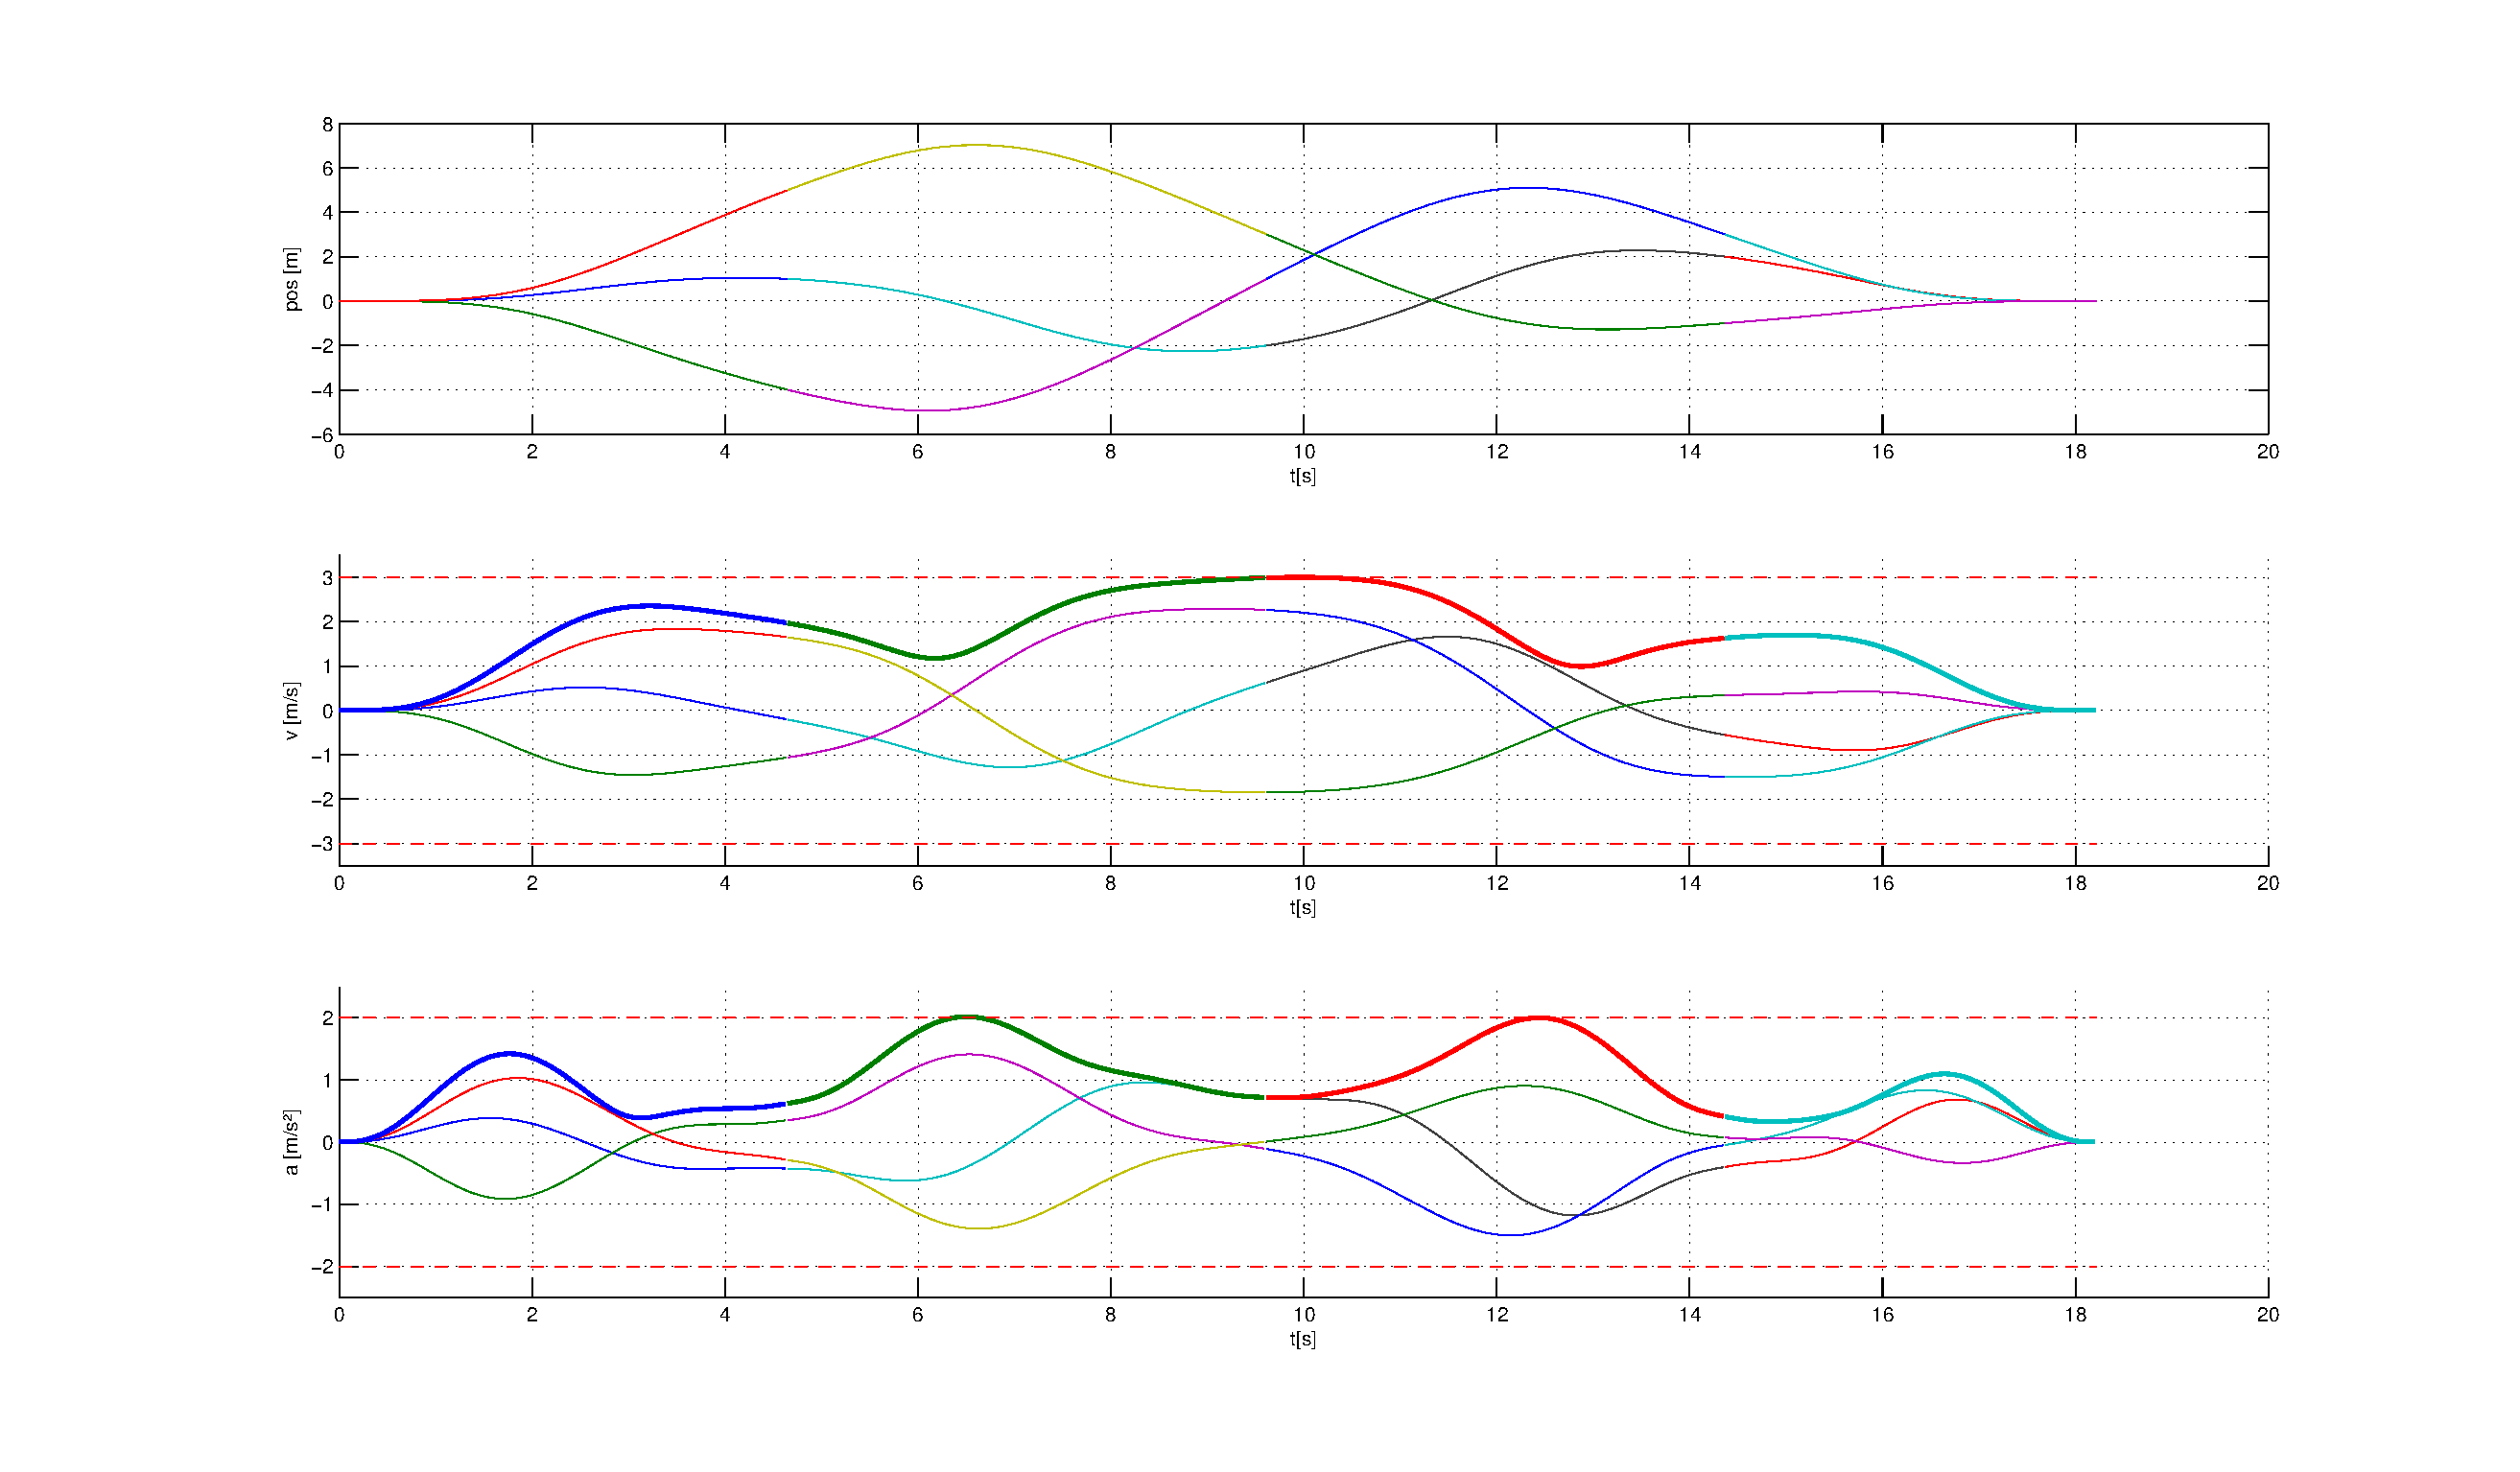
\includegraphics[width=1\textwidth]{pics/optimized.eps}
%   \caption{Ein Bild.}
%\end{figure}
%
%
%\begin{figure}[h]
%   \centering
%   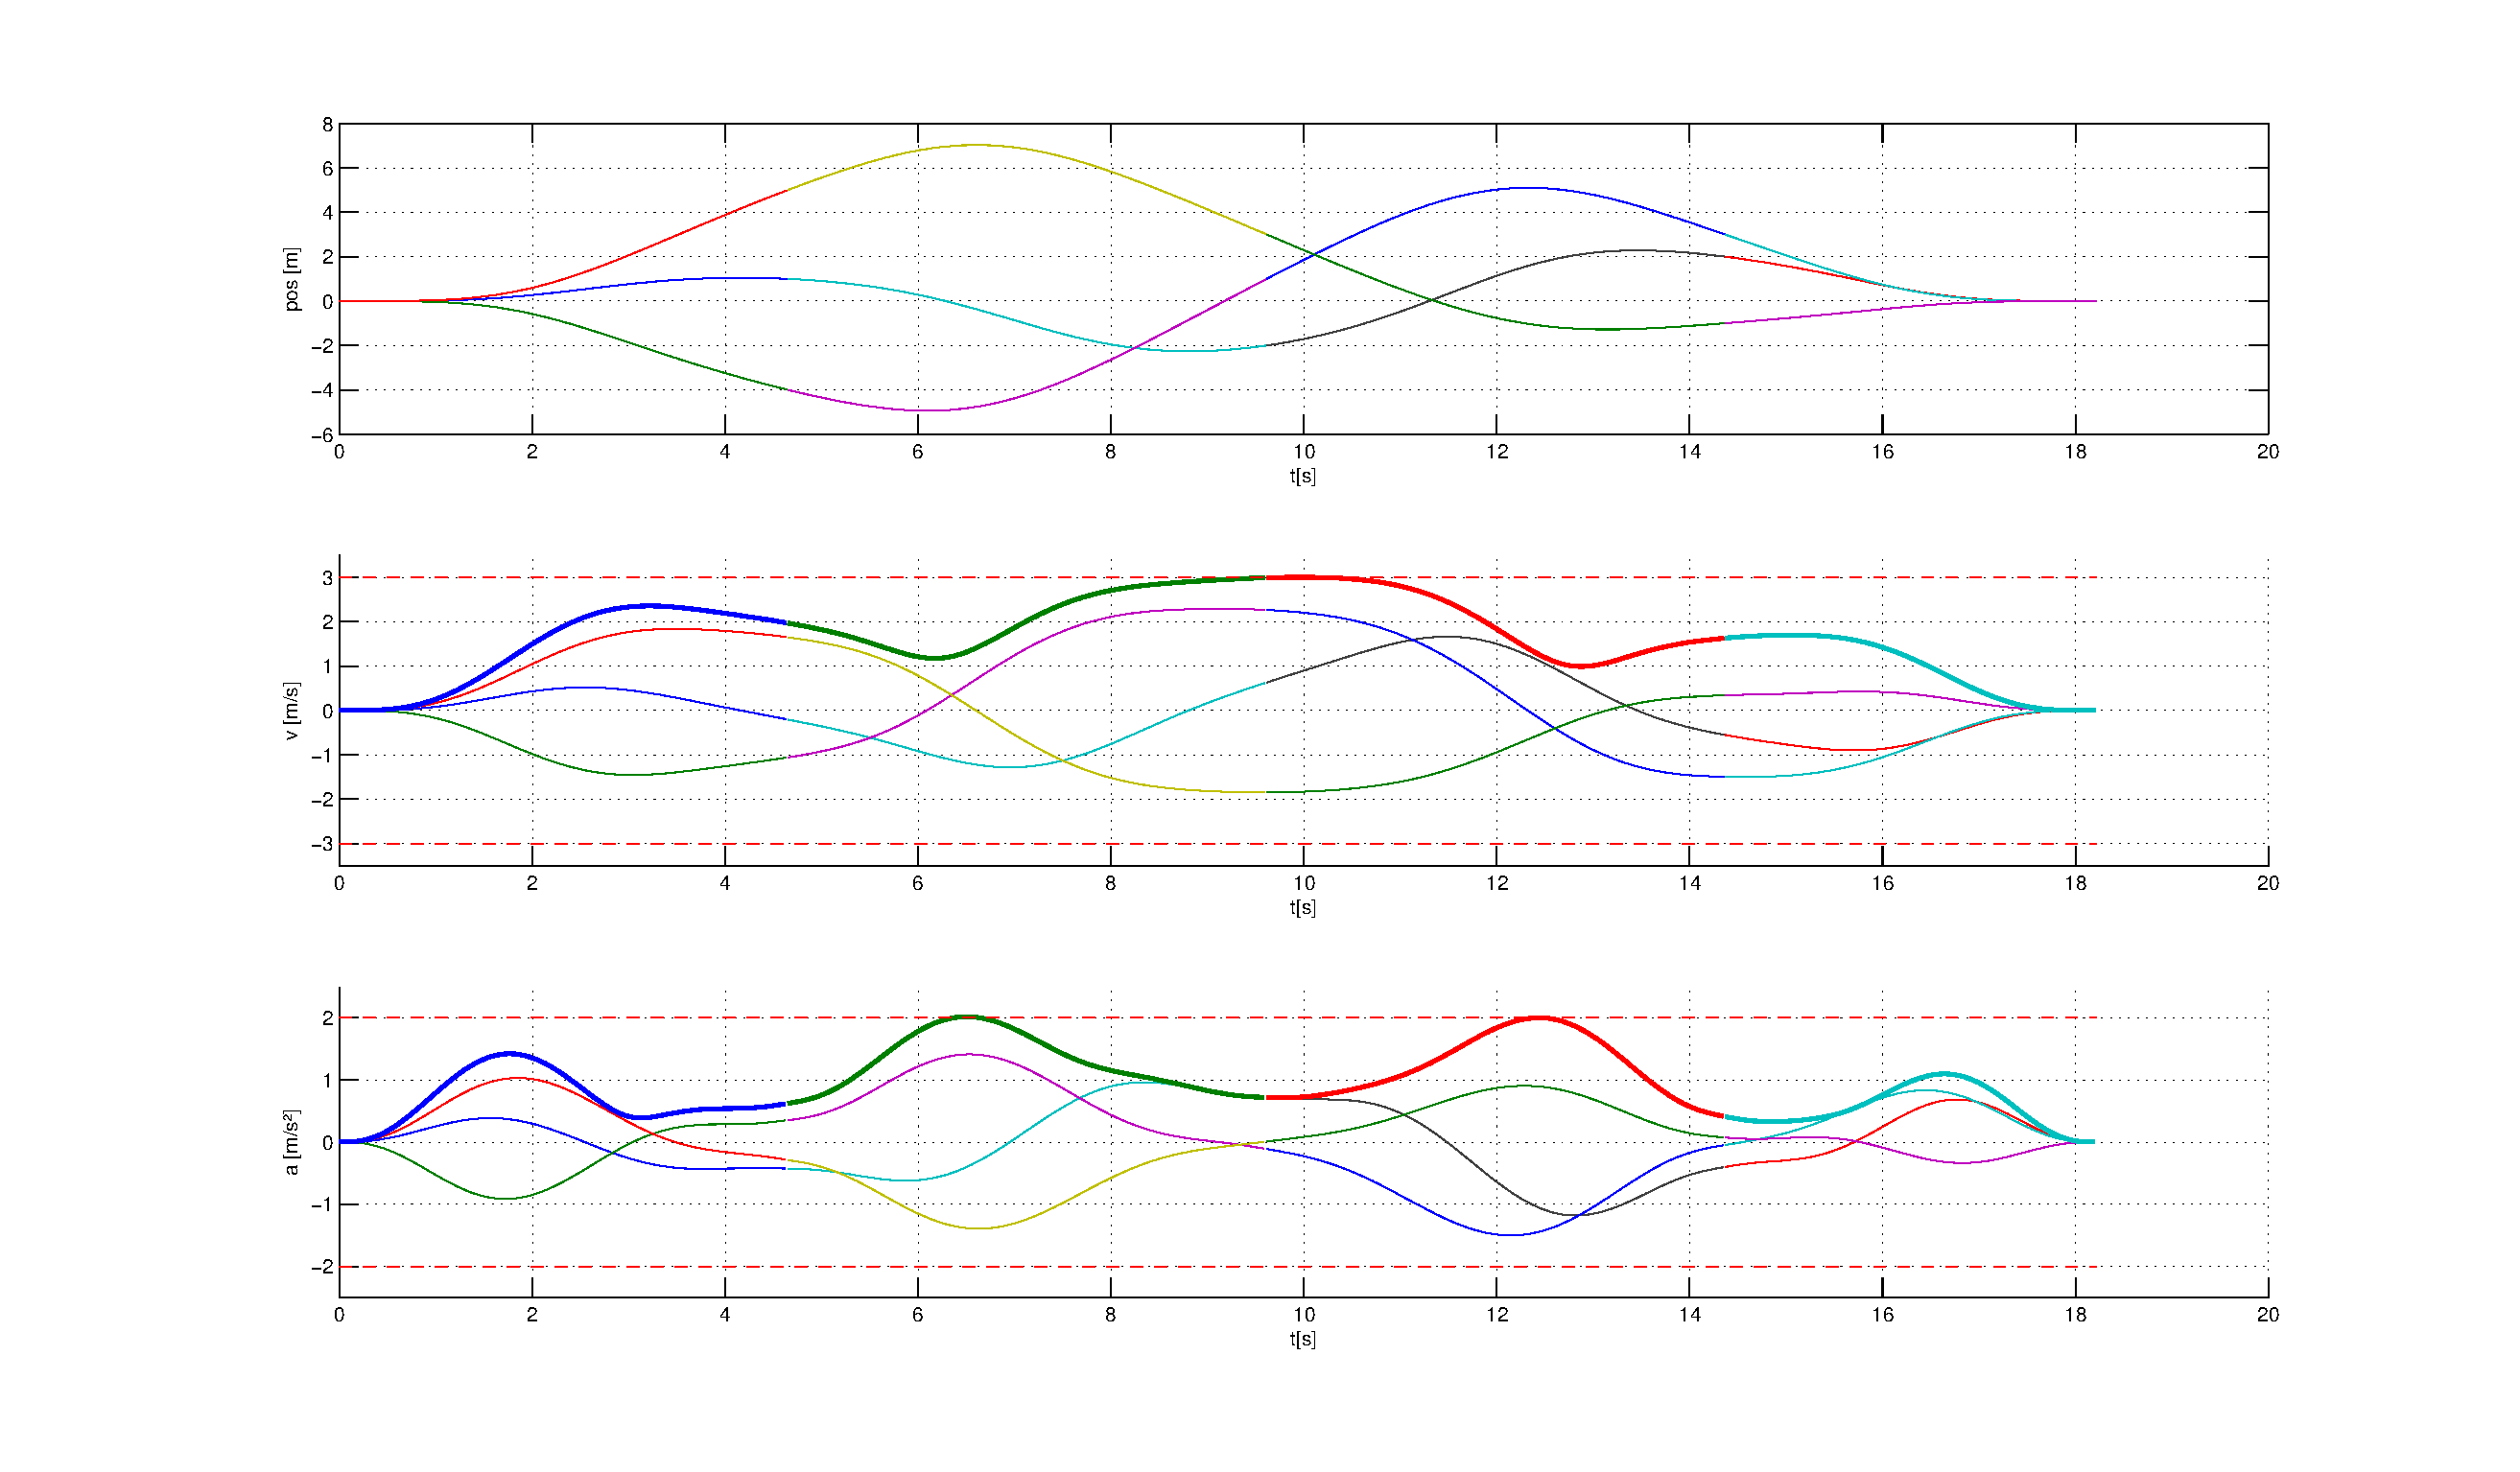
\includegraphics[scale=0.3]{pics/optimized.eps}
%   \caption{Ein Bild.}
%\end{figure}



%\begin{figure}[h]
%   \centering
%   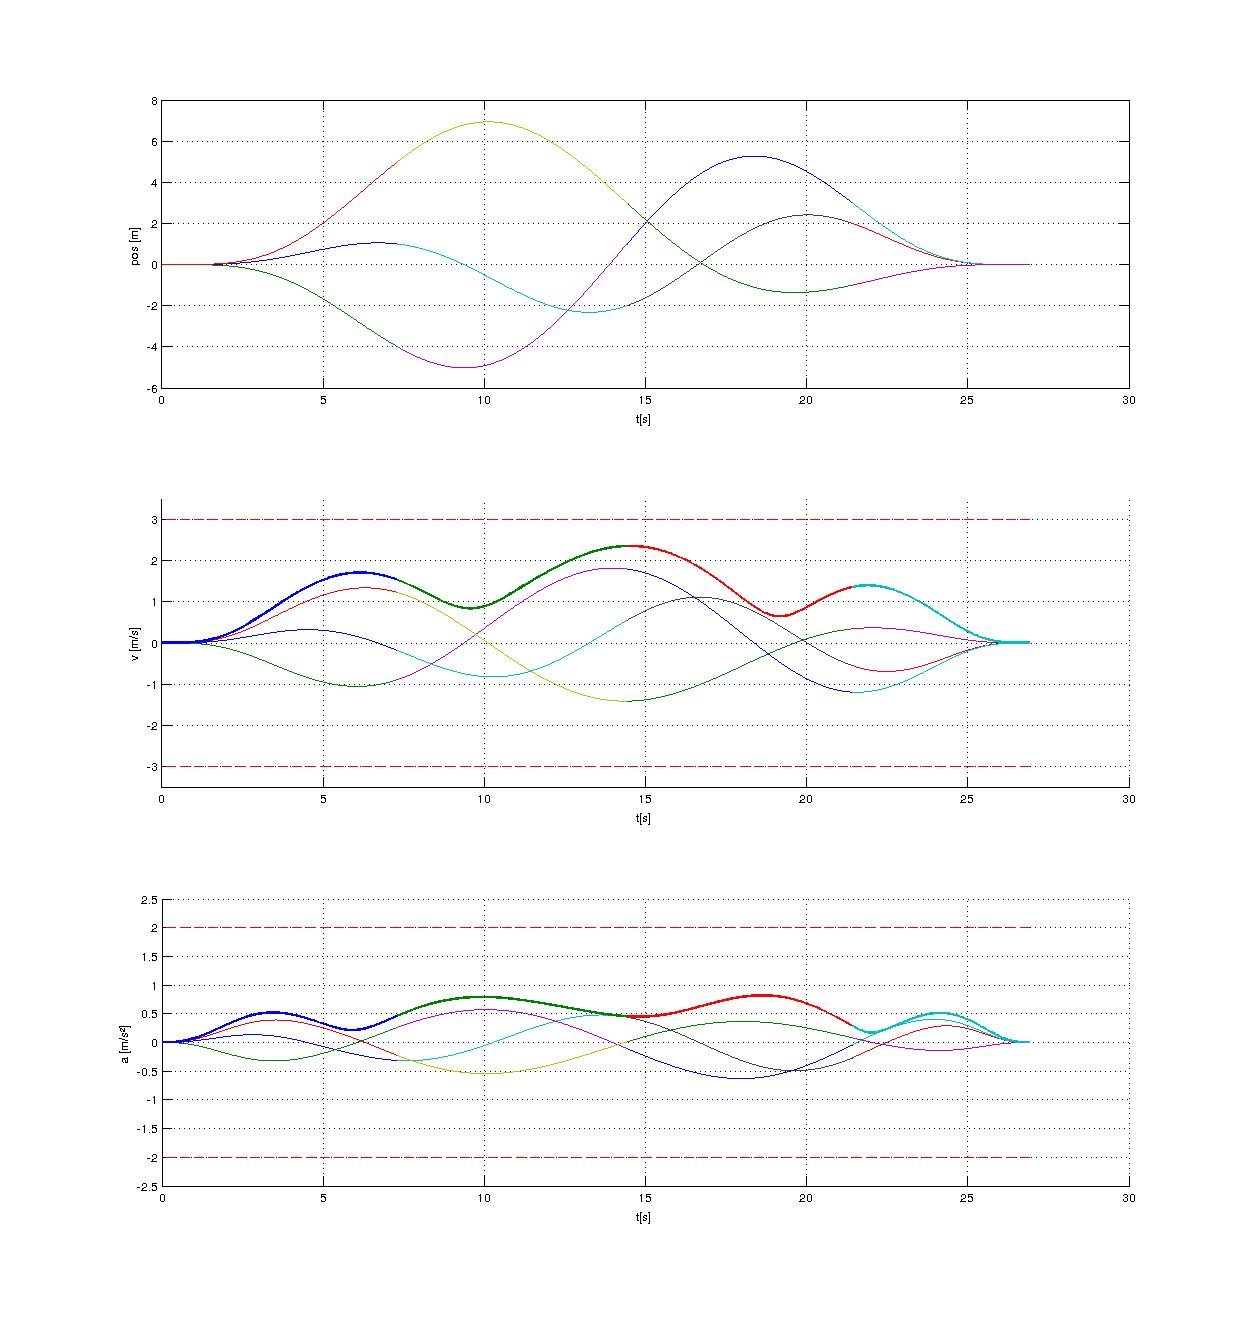
\includegraphics[width=1\textwidth]{pics/initial.eps}
%   \caption{Ein Bild.}
%\end{figure}

%\begin{figure}[h]
%   \centering
%   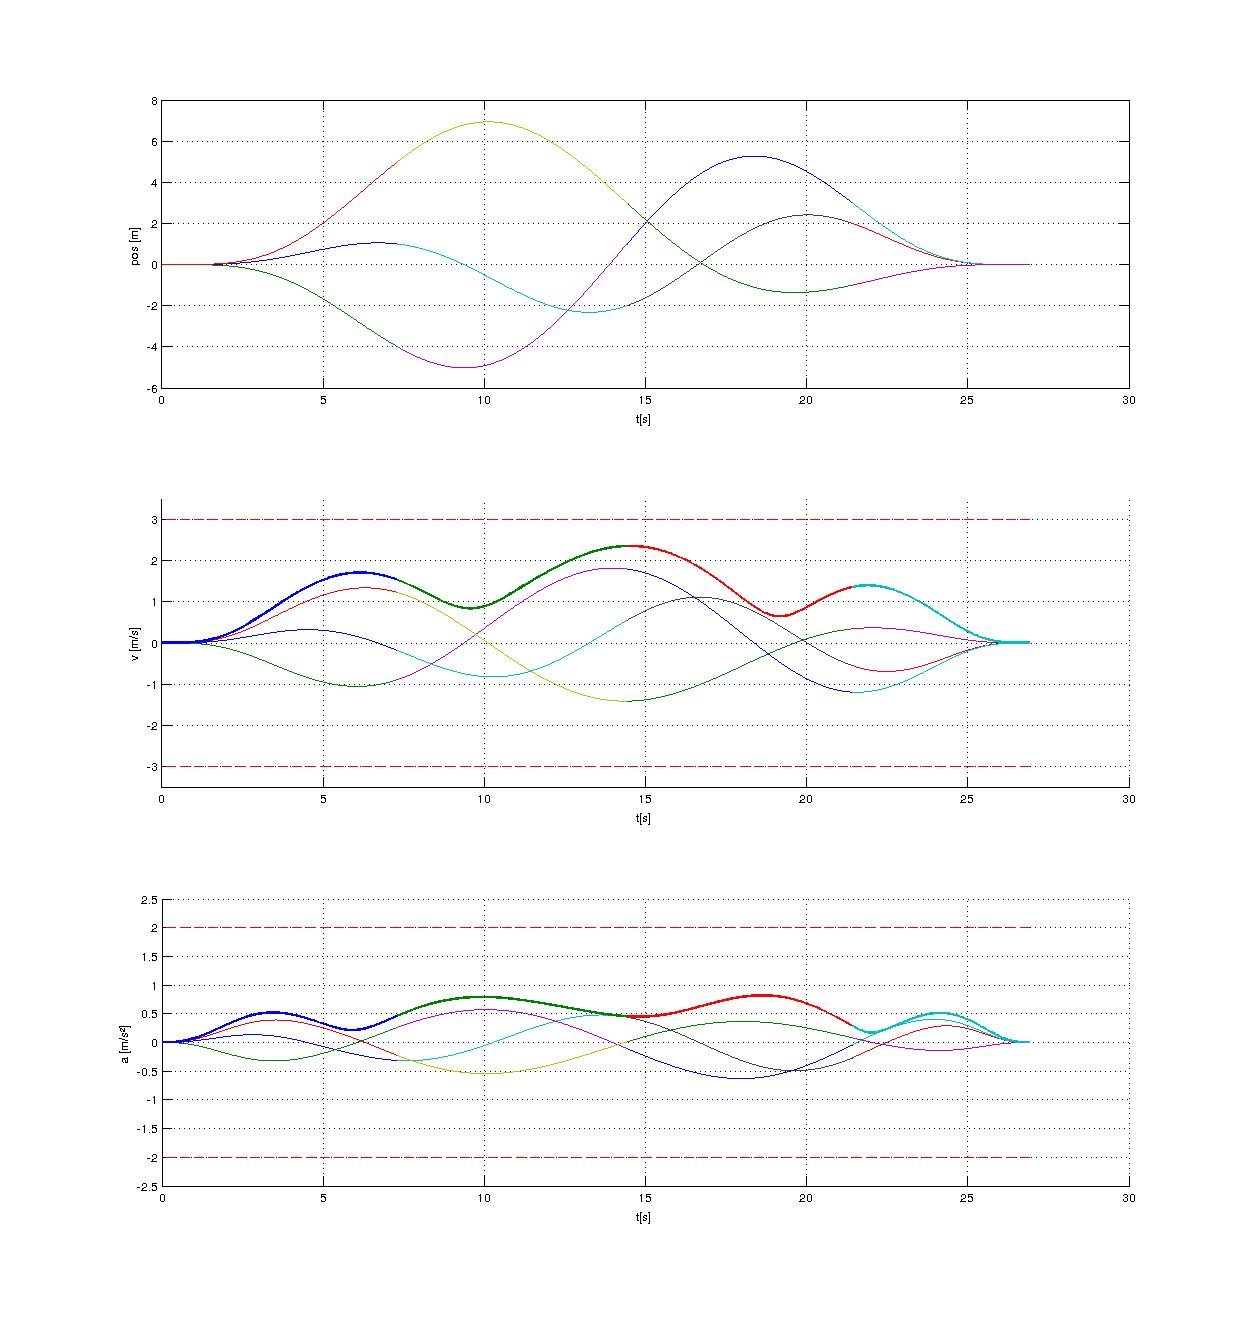
\includegraphics[scale=1]{pics/initial.eps}
%   \caption{Schematic of a rough foot surface.}
%   \label{pics:profile2}
%\end{figure}
























 \cleardoublepage
 \chapter{RRT}\label{chap:RRT}

\section{General}

The goal of this thesis was not only to generate a numerically stable, snap optimized polynomial trajectory but also to explore a densely packed (indoor) environment and plan an aggressive trajectory in between the obstacles. Hence, the Rapidly-Exploring Random Tree (RRT) algorithm is used to find a collision-free straight line solution through densely packed environments. The sampling points oft the RRT (or RRT*) algorithm are then used as the vertices in the polynomial optimization.


\section{RRT Algorithm}\label{sec:RRT}

RRT is a computational efficient algorithm to find a path in a high dimensional space by randomly building a space-filling tree. The sampling points are drawn randomly from the sample space and the tree grows incrementally. 
For each new sample the algorithm attempts to build a collision-free connection to the nearest state in the tree. If a collision-free connection is possible the sample and the connection are added to the tree. \newline

An iteration of the RRT algorithm can be depicted schematically:


\begin{enumerate}
  \item Generate a random sample
  \item Find nearest state in tree
  \item Try to build a collision-free connection to the nearest state
  \item If feasible, add the sampled state and the connection to the tree
\end{enumerate}

\subsection{Goal State}

As mentioned above, the RRT algorithm is based on random samples. Therefore it is very unlikely that a sampled state perfectly matches the desired goal state. \newline

There are two different strategies to enable the RRT algorithm to get to the goal. One strategy is to define not only a goal state but a goal region. Every random sample which is located within the goal region is considered a goal state. As soon as a collision-free connection to a sample in the goal region is established, this trajectory is stored as the best trajectory. At this point the algorithm can be stopped or further iteration can be performed to find a better trajectory to the goal region. Once an other state from the goal region is sampled and the cost of the path to the new state is lower then the cost of the best trajectory, the best trajectory is replaced by the new path. \newline
Another strategy is to steer the RRT algorithm directly to the goal state. In addition to the randomly sampled states the exact goal state is added to the algorithm. The schematic description of an iteration of the RRT algorithm listed in section \ref{sec:RRT} can be modified to represent an iteration with the goal state:

\begin{enumerate}
  \item Insert goal state
  \item Find nearest state in tree
  \item Try to build a collision-free connection to the nearest state
  \item If feasible, add the sampled state and the connection to the tree
\end{enumerate}

In all the cases where a direct collision-free connection between start and goal state is not possible the iteration with the goal state will not succeed in a first attempt. Hence the iterations with the randomly sampled states described in section \ref{sec:RRT} are needed to build the space filling tree.\newline

Figure \ref{pic:smallGamma} depicts the straight line solution of the RRT algorithm with a fixed goal state. The figure is in bird's eye perspective and shows a crossing of different hallways. The blue cells represents the floor and the green cells represents the walls. The map was generated with a stereo camera and was not reworked. Therefore some of the cells of the floor which should be occupied/blue are left free. 

\begin{figure}[H]
   \centering
   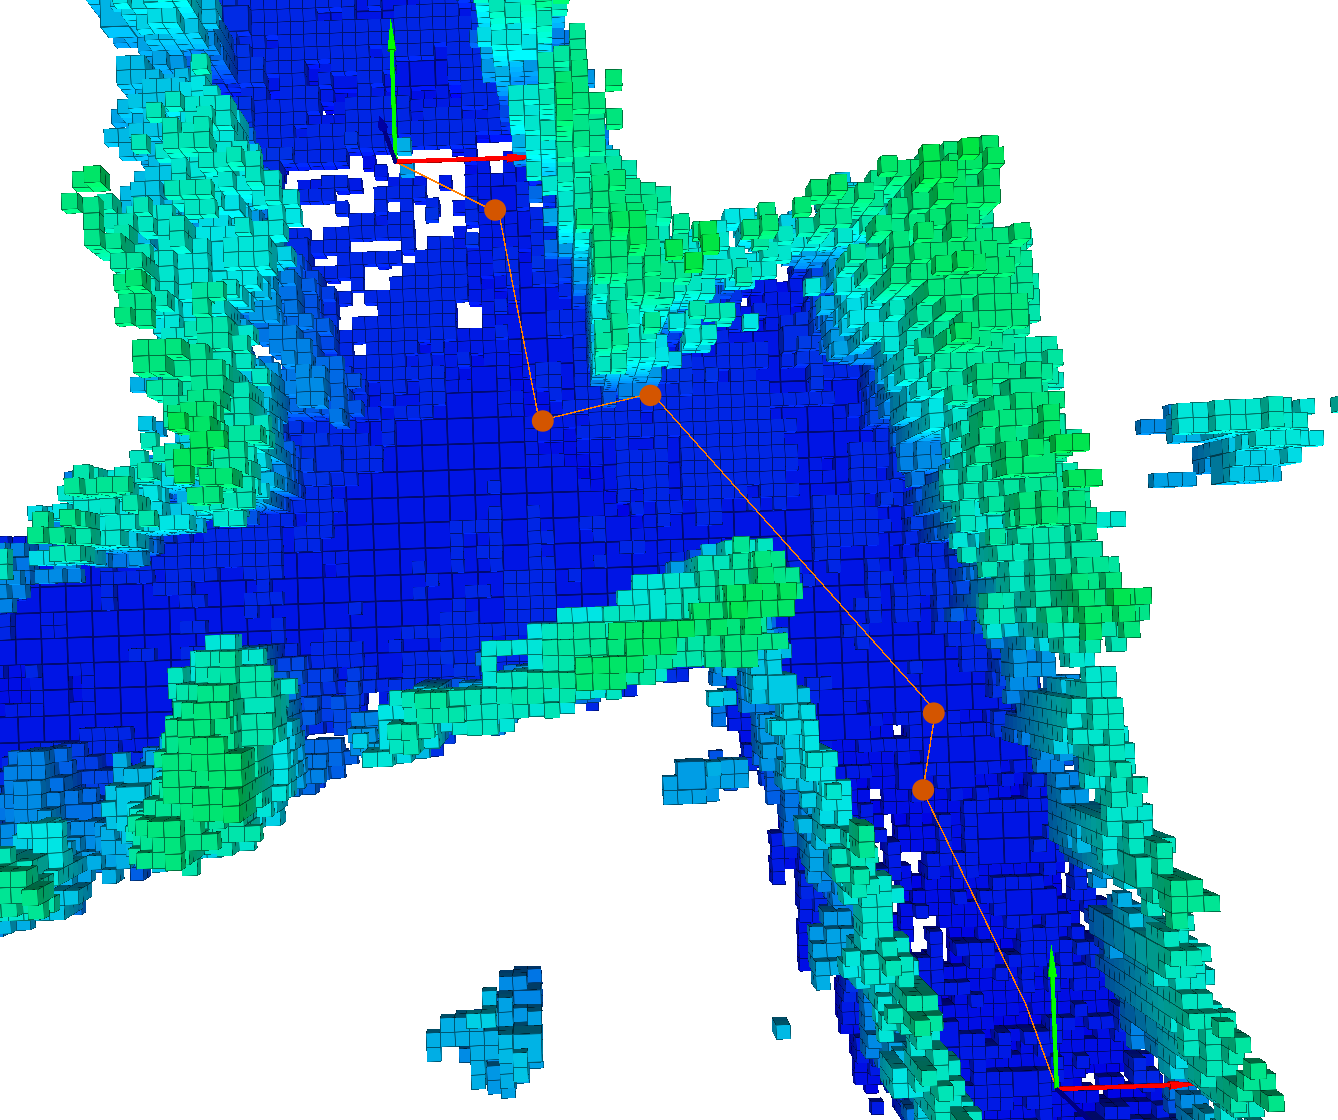
\includegraphics[trim = 50mm 0mm 30mm 0mm,clip,width=0.8\textwidth]{pics/smallGammaP.png}
   \caption{Straight line solution of the RRT algorithm with a fixed goal state. Start and goal state are each represented by a red $x$-vector and a green $y$-vector. The random sampled states are depicted as orange dots.}
   \label{pic:smallGamma}
\end{figure}



\section{RRT* Algorithm}\label{sec:RRTstar}

In contrast to the RRT algorithm the RRT* (or RRT Star) algorithm not only tries to connect to the nearest state in the tree but to several states near the sampled state. The user can define a threshold (on the distance) which defines which states of the tree belongs to the "near states". If there is no state within the user specified range the algorithm attempts to build a collision-free connection to the nearest state in the tree just as the RRT algorithm.  \newline
As a first step, the sampled state is connected to the best state among the near states whereas best means minimum cost/distance. Once the sampled state is added to the tree all the other states among the set of near states are connected to the sampled state. If the connection is collision-free and the cost of the total path is smaller than the cost of the existing path, the old path is replaced. \newline

An iteration of the RRT* algorithm can be depicted schematically:


\begin{enumerate}
  \item Generate a random sample
  \item A threshold defines a set of near states
  \item Try to build a collision-free connection to best state among the near states
  \item Add the sampled state and the connection to the tree 
  \item Try to connect all the other states from the set with the sampled state 
  \item Replace the old path if the new one has a smaller cost
  \item If there is no near state within the threshold apply the RRT algorithm
\end{enumerate}


Because the RRT* algorithm tries to connect to several states each iteration, the procedure to find a path takes longer and is computationally more expensive. However, solutions with lower cost can be found which is more important for most real life applications.

\subsection{Rewiring}

The sequence of step 5 and step 6 of the RRT* algorithm ("Try to connect all the other states from the set with the sampled state", "Replace the old path if the new one has a smaller cost") are called "rewiring". \newline 
The threshold which defines the set of near states depends on a user specified parameter $\gamma$. In this case, the threshold is the radius of a sphere, i.e. all the near states are located within this sphere. The radius $r$ can be calculated according to


\begin{equation}
r = \gamma * \left(\frac{ln(n+1)}{n+1}\right)^{1/d}
\label{equ:ballradius}
\end{equation}

where $n$ is the number of states which are already in the tree. The dimension of the state space $d$ is a fixed parameter and $ln$ represents the natural logarithm.\newline

As mention in section \ref{sec:RRTstar} the RRT* algorithm is computationally more expensive but returns trajectory with lower cost. Both aspects are caused by the rewiring and are therefore strongly influenced by the parameter $\gamma$. A large $\gamma$ defines a large sphere, hence it is likely to have more states (which are already in the tree) to be located within the sphere. The rewiring of the near states tends to result in shorter trajectories with fewer segments.

Figure \ref{pic:smallBBX} depicts the straight line solution of the RRT* algorithm with a fixed goal state. Compared to figure \ref{pic:smallGamma} a superior trajectory is found since a rewiring of the states in the tree was performed.

\begin{figure}[H]
   \centering
   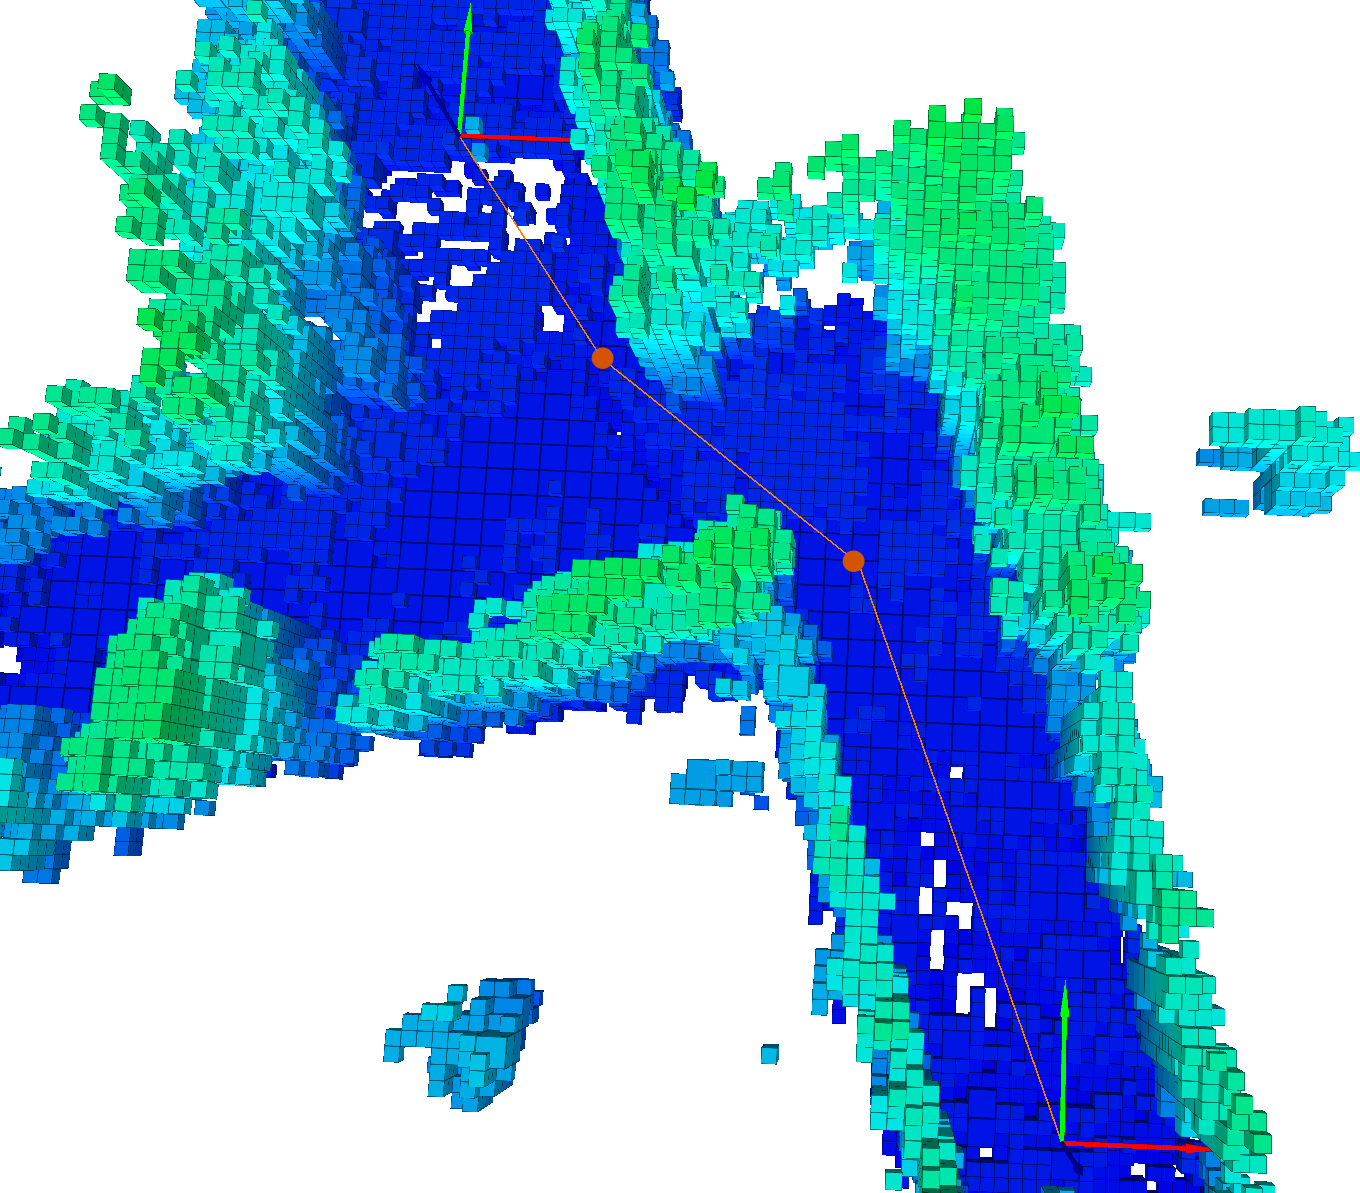
\includegraphics[trim = 50mm 0mm 30mm 0mm,clip,width=0.8\textwidth]{pics/smallBBXP.png}
   \caption{Straight line solution of the RRT* algorithm with a fixed goal state. Start and goal state are each represented by a red $x$-vector and a green $y$-vector. The random sampled states are depicted as orange dots. The $\gamma$ parameter in this example was set to $\gamma = 1.5$.}
   \label{pic:smallBBX}
\end{figure}


\subsection{Bounding Box}\label{sec:bbx}

The straight line solution in figure \ref{pic:smallBBX} is collision-free but passes by very close to the walls. In real life application not only a point mass but a object (in this master thesis a UAV) should follow the trajectory. Therefore a bounding box is installed around the trajectory. \newline
The bounding box is implemented as a cuboid. The 3 dimension of the cuboid can be defined individually. The trajectory is then divided into a discrete trajectory and the bounding box is installed around the discrete points. If there is a obstacle in one of the bounding boxes the hole straight line is considered as  in collision. \newline

Figure \ref{pic:bbx} depicts the straight line solution of the RRT* algorithm with a bounding box. In contrast to figure \ref{pic:smallBBX} the trajectory is now located more central in the hallway because the bounding box makes it impossible to pass by the wall very close. Because the trajectory proceeds less direct from start to goal state the total distance of the trajectory increases. 

\begin{figure}[H]
   \centering
   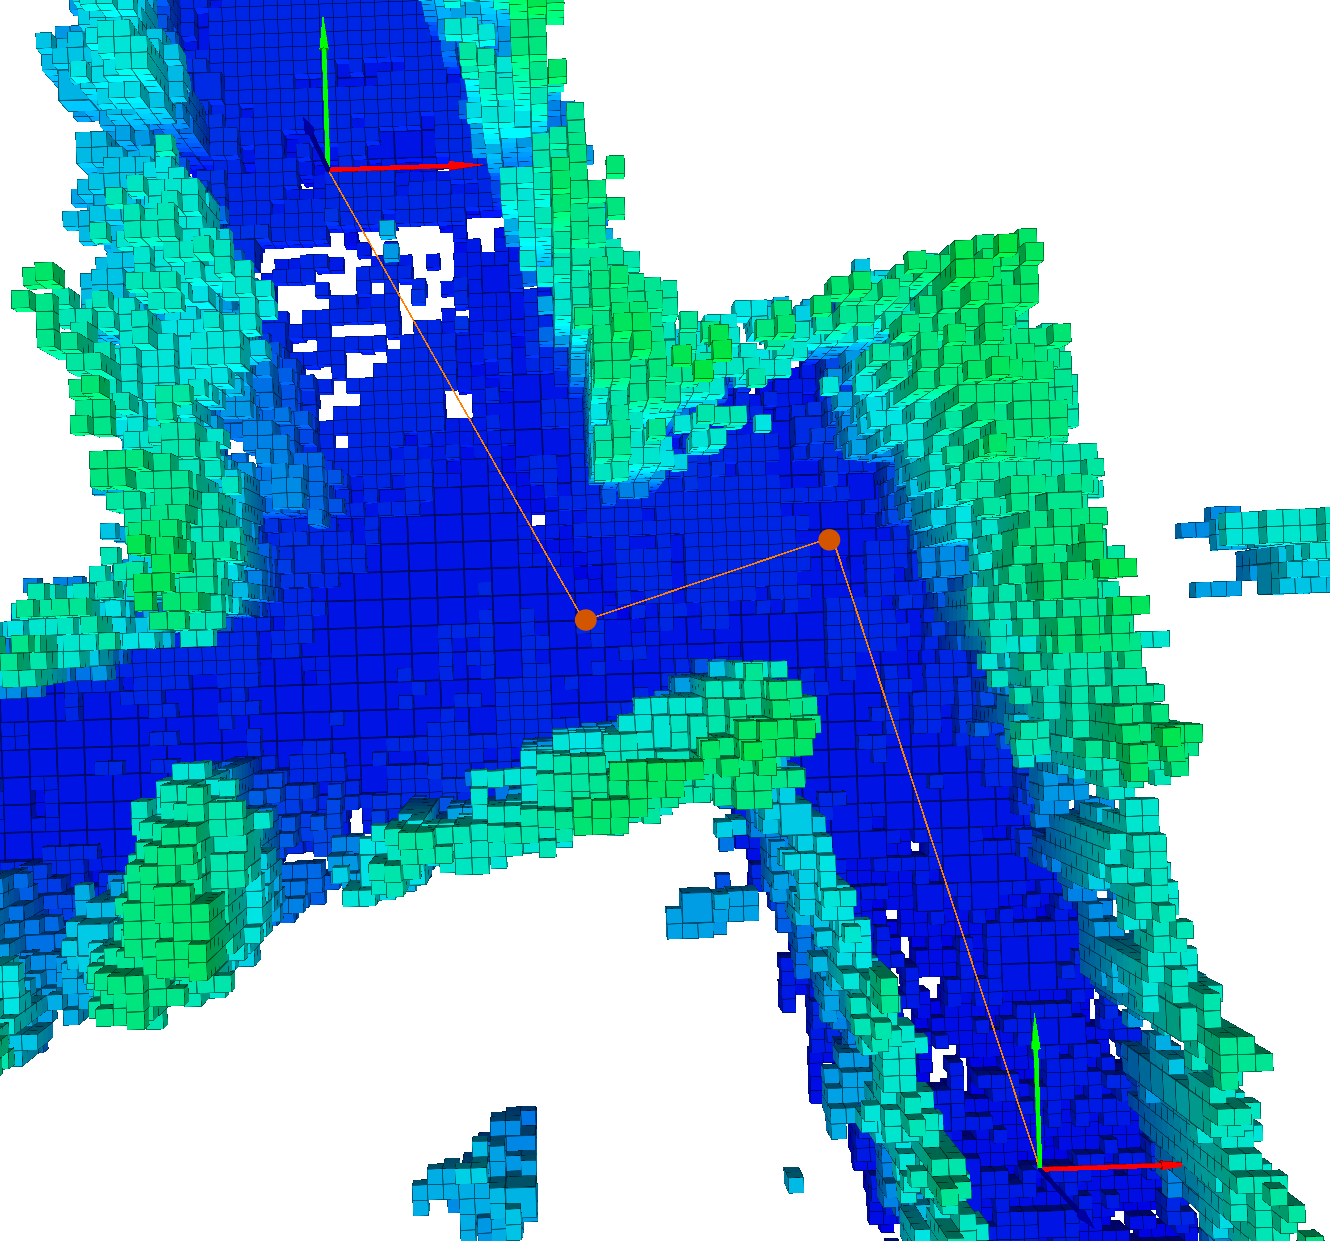
\includegraphics[trim = 50mm 0mm 30mm 0mm,clip,width=0.8\textwidth]{pics/largeBBXP.png}
   \caption{Straight line solution of the RRT* algorithm with bounding box. Due to the bounding box the trajectory is located more central in the hallway because the bounding box makes it impossible to pass by the wall very close. The $\gamma$ parameter in this example was set to $\gamma = 1.5$.}
   \label{pic:bbx}
\end{figure}

\subsection{Ray Check}

 TODO: verbindung zu Octompa
 
 matlab figure



%\begin{figure}[h]
%   \centering
%   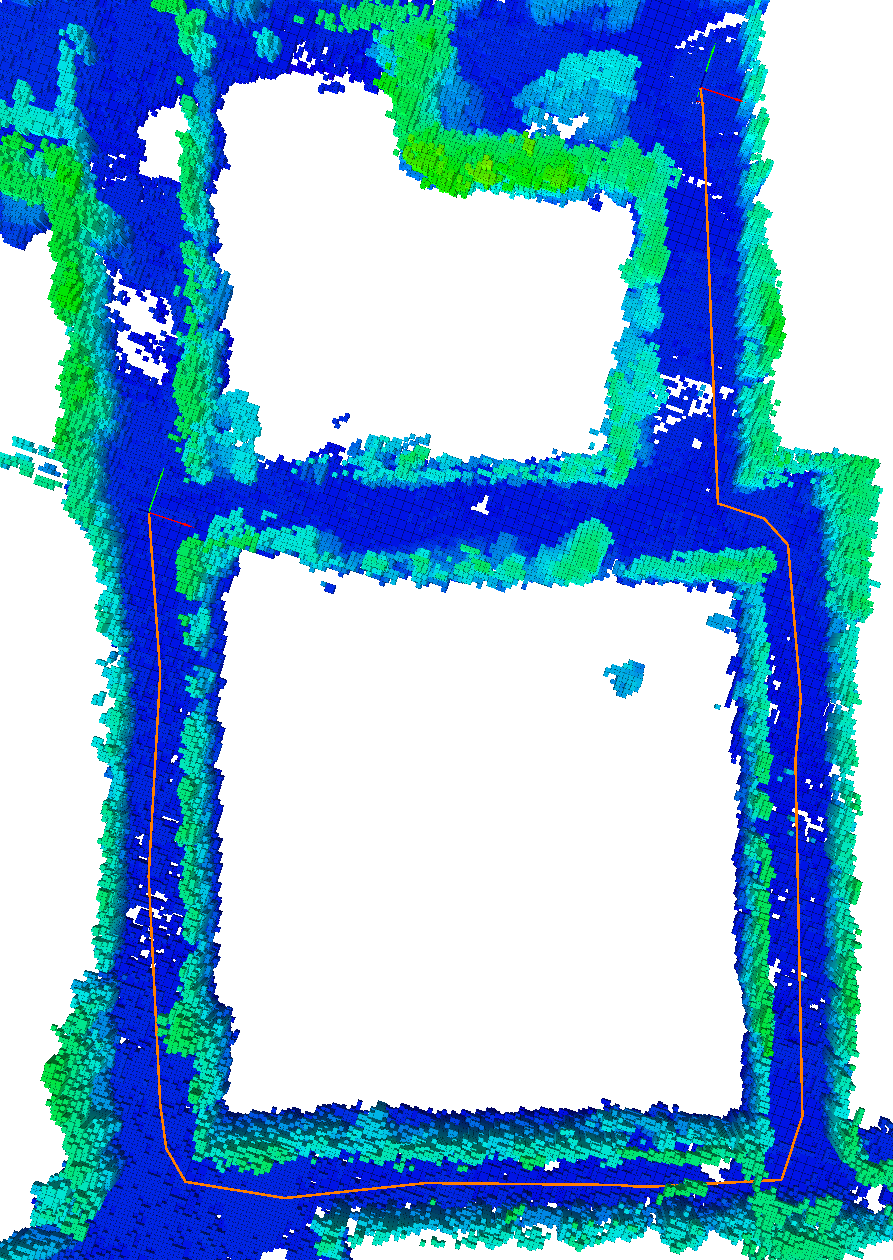
\includegraphics[width=1\textwidth]{pics/MapLine.png}
%   \caption{Ein Bild.}
%\end{figure}



%\begin{figure}[h]
%   \centering
%   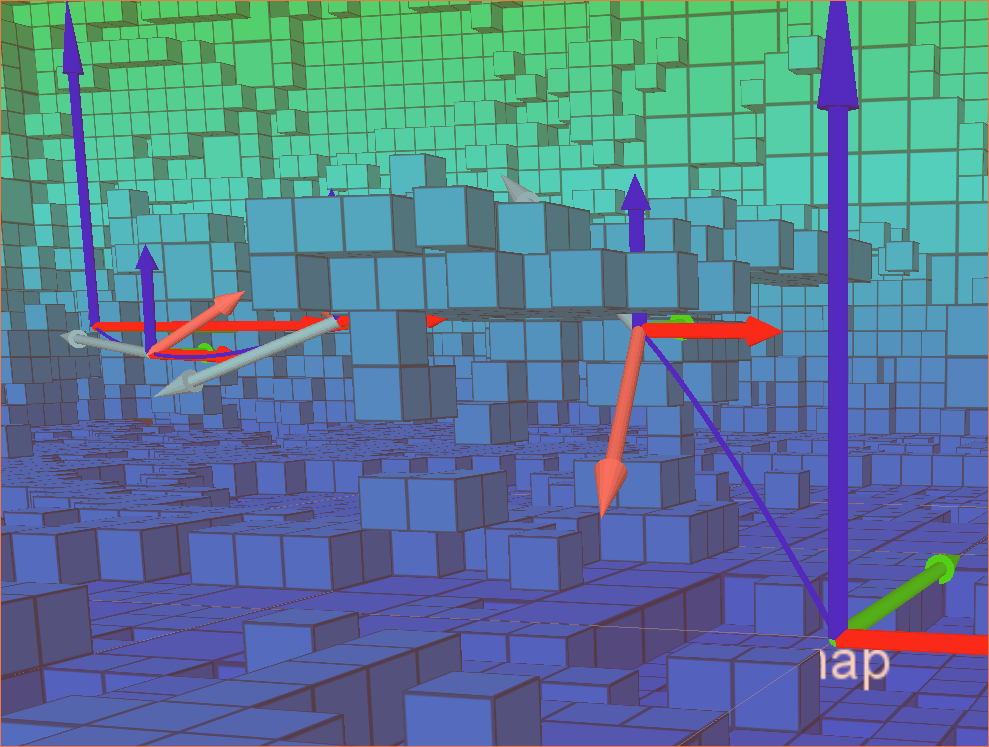
\includegraphics[width=1\textwidth]{pics/initialSolution.png}
%   \caption{Ein Bild.}
%\end{figure}
%
%
%\begin{figure}[h]
%   \centering
%   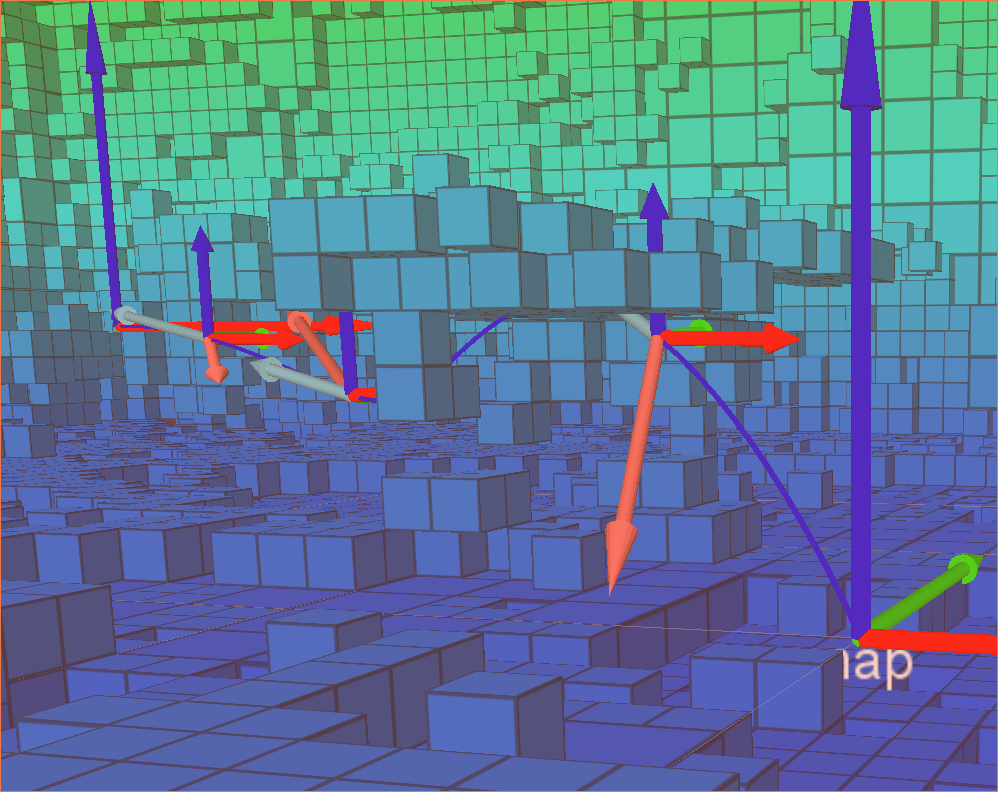
\includegraphics[width=1\textwidth]{pics/Vertex_in_middle_2.png}
%   \caption{Ein Bild.}
%\end{figure}
%
%\begin{figure}[h]
%   \centering
%   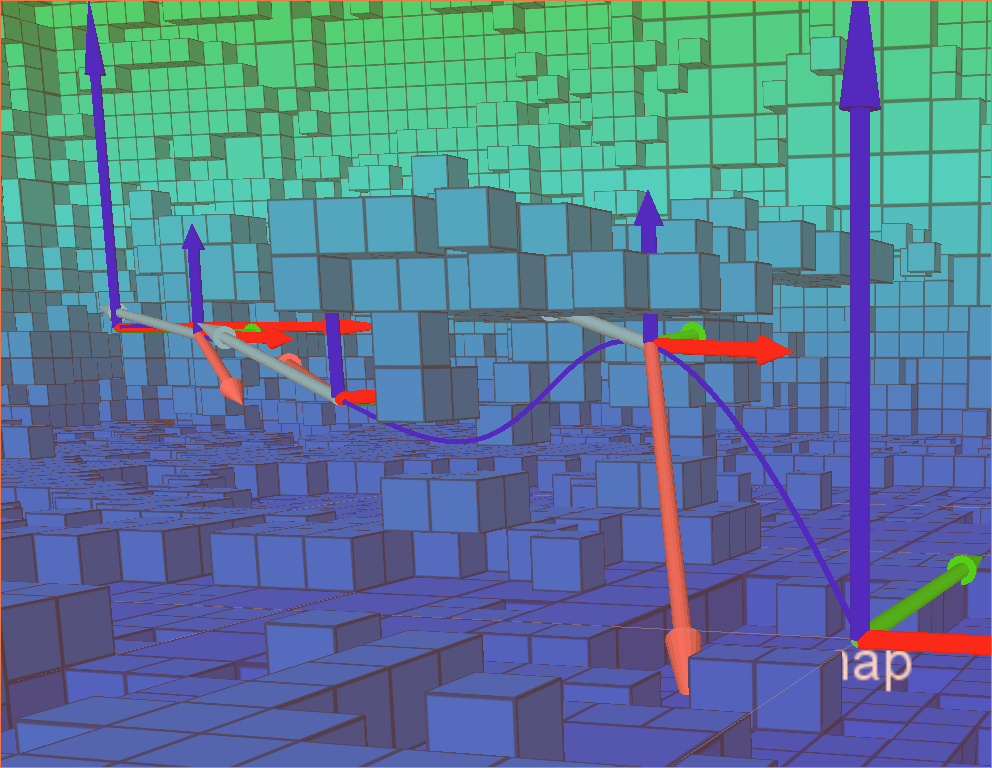
\includegraphics[width=1\textwidth]{pics/section.png}
%   \caption{Ein Bild.}
%\end{figure}
%
%
%\begin{figure}[h]
%   \centering
%   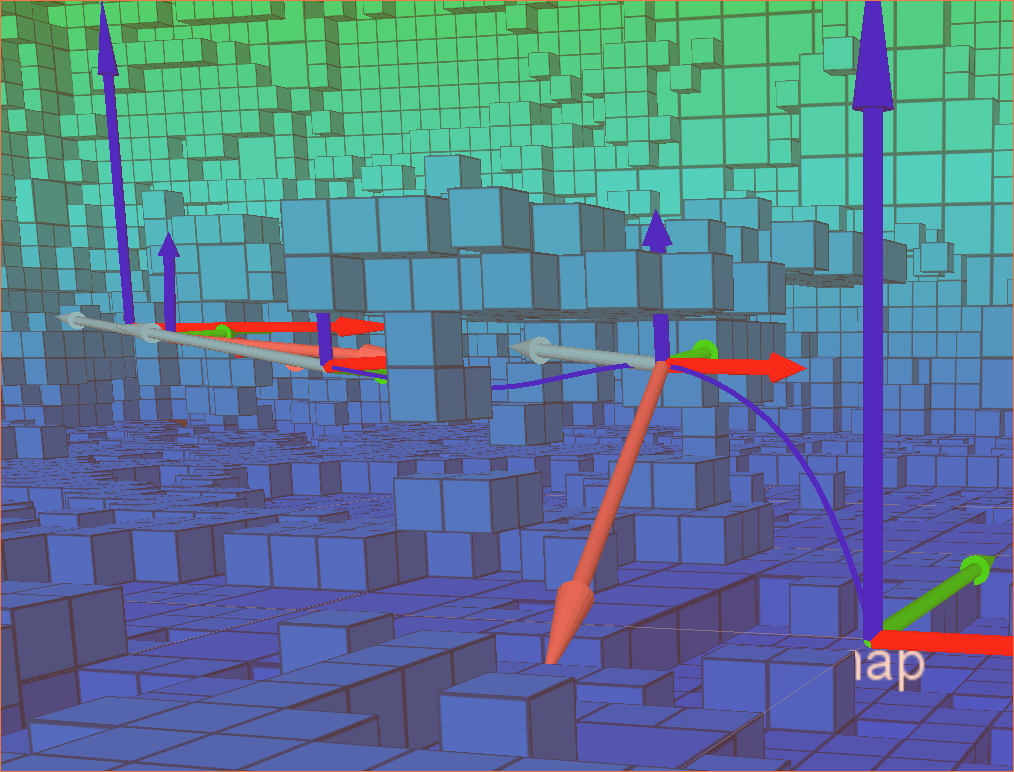
\includegraphics[width=1\textwidth]{pics/Nlopt_after_sectionAndTime.png}
%   \caption{Ein Bild.}
%\end{figure}
 \cleardoublepage
  \chapter{Path Planning}\label{chap:Planning}

\section{Usage of the RRT* Vertices}

Chapter \ref{sec:trajectory} illustrates the optimization of a trajectory which passes through predefined vertices. From now on, the vertices are no longer chosen manually but are defined by the result of the RRT* algorithm. The computational efficiency of the RRT* algorithm combined with the positive features of the nonlinear optimization discussed in section \ref{sec:nonlinearopt} will lead to a optimized trajectory in densely packed environment.

\subsection{Vertex Extension}


Since the RRT* algorithm does not consider the dynamical behavior of a UAV there are still some challenges converting the RRT* straight line solution into a polynomial trajectory. In other words, there is the possibility that the polynomial trajectory passing through the vertices of the collision-free straight line solution is in collision with an obstacle. In this case a vertex, which is located on the straight line, has to be added. \newline

The process of generating a collision-free optimized trajectory can be summarized in following steps:


\begin{enumerate}
  \item Generate a collision-free straight line solution using the RRT* algorithm
  \item Create an initial trajectory passing through the vertices of the straight line solution
  \item If the initial solution is in collision, extend the existing vertices by a vertex located on the straight line solution. Compute the initial solution including the new vertex. Repeat this step until the trajectory is collision-free
\item Perform a nonlinear optimization on the collision-free trajectory
\item If the optimized solution is in collision, extend the existing vertices by a vertex located on the straight line solution and restart the nonlinear optimization. Repeat this step until the optimized trajectory is collision-free
\end{enumerate}

This schematic description of the process is depicted step by step in the subsequent figures for a better understanding.

\subsubsection{1. Generate a collision-free straight line solution using the RRT* algorithm}

Figure \ref{pic:RRTstepOne} depicts the straight line solution of the RRT* algorithm, which is explained in section \ref{sec:RRTstar}.  The $\gamma$ parameter, which is needed to calculate the radius $r$ in equation \ref{equ:ballradius}, is set to $\gamma = 1.5$. Furthermore, the edge length of the bounding box is set to $0.5m$ for each dimension. Although the hight of a UAV is commonly smaller than the length and the width this is required if great roll and pitch angles are permitted. \newline


Please note that, due to the randomness of the RRT* algorithm, the straight line solution depicted in figure  \ref{pic:RRTstepOne} is different than the straight line solution depicted in figure \ref{pic:bbx} even though the parameters are the same. 

\begin{figure}[h]
   \centering
   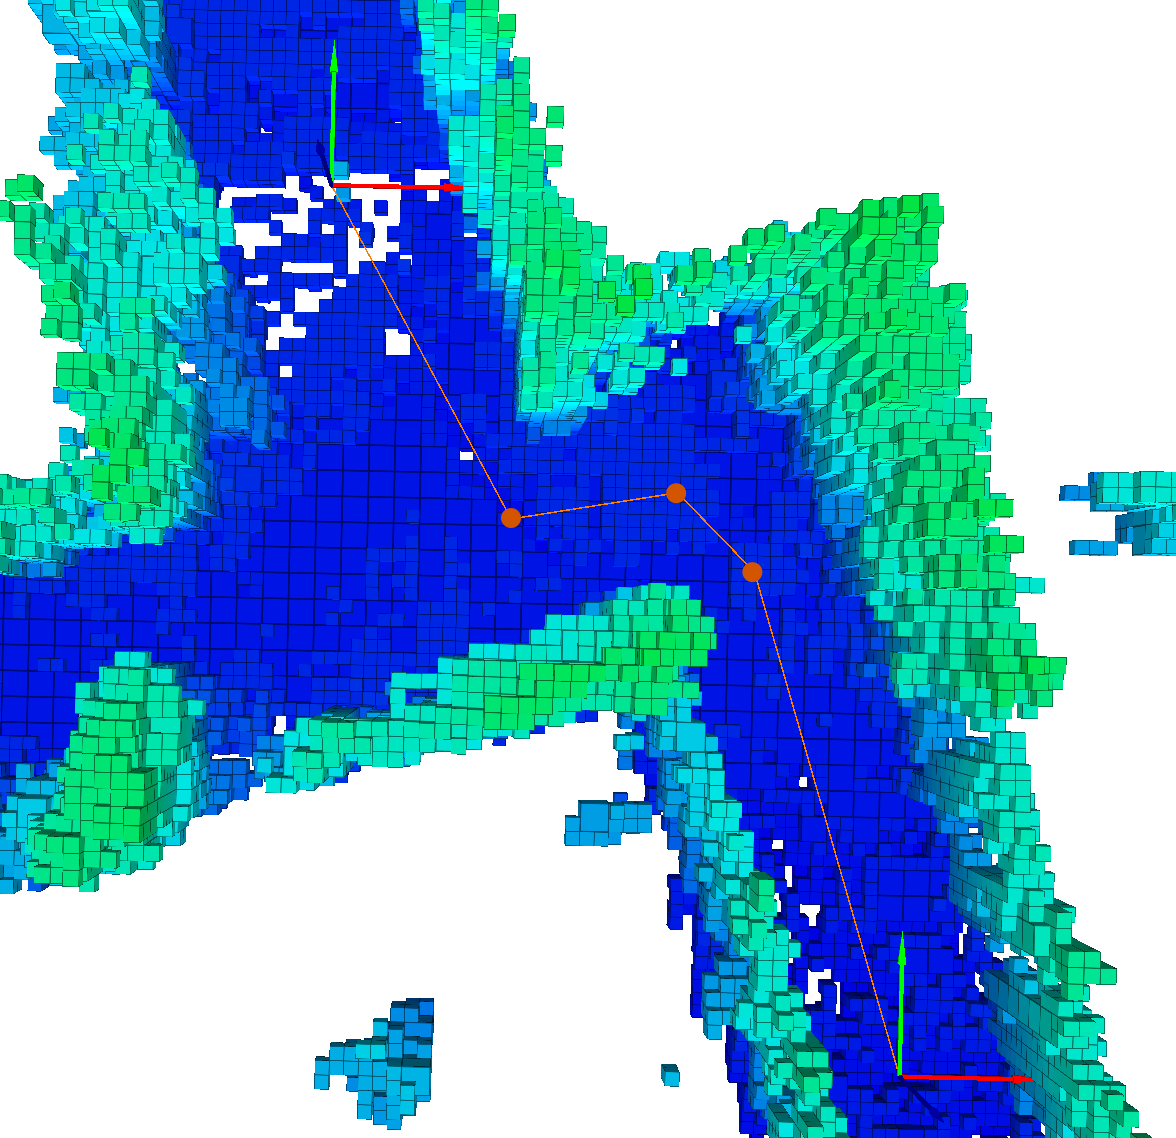
\includegraphics[trim = 45mm 0mm 35mm 0mm,clip,width=0.8\textwidth]{pics/extensionLongP.png}
   \caption{A collision-free straight line solution with 4 segments.}
   \label{pic:RRTstepOne}
\end{figure}


\subsubsection{2. Create an initial trajectory passing through the vertices of the straight line solution}

The start and goal vertex (each marked by a red and green arrow in figure \ref{pic:RRTstepOne}) as well ass the 3 vertices (each marked by a orange dot in figure \ref{pic:RRTstepOne}) defined by the solution of the RRT* algorithm are now used to generate the initial polynomial solution according to equation \ref{equ:dpstar} and equation \ref{equ:segmentTime}. \newline

The initial trajectory passing through the vertices of the RRT* algorithm is depicted in figure \ref{pic:RRTstepTwo}. The start vertex is in the upper left corner and the goal vertex is in the lower right corner. In the second segment there is a collision between the trajectory and the wall of the hallway (represented by green boxes). 

\begin{figure}[h]
   \centering
   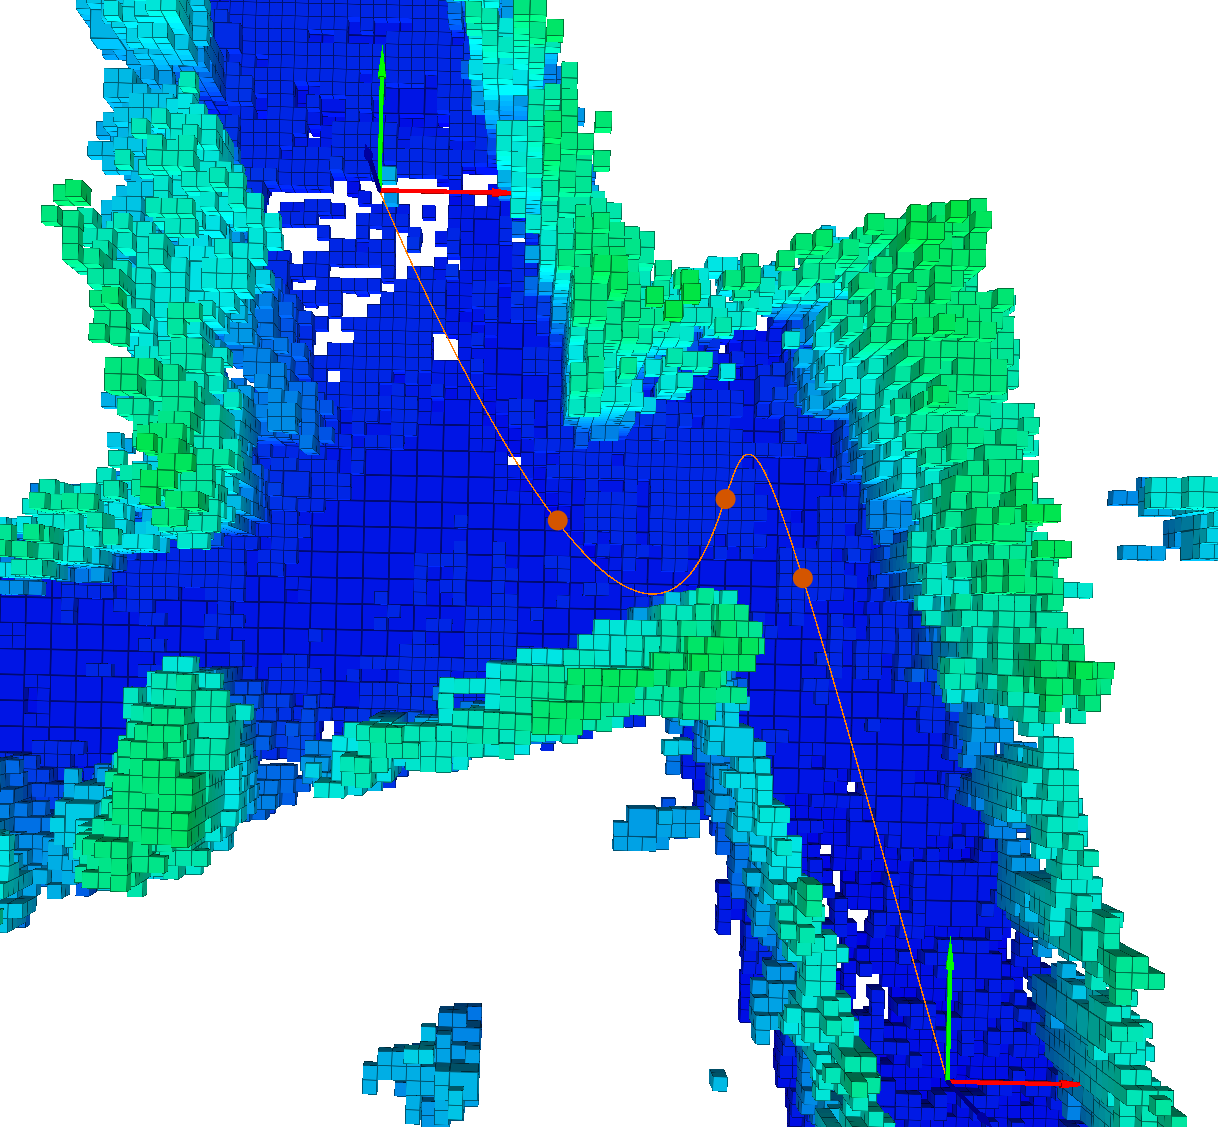
\includegraphics[trim = 45mm 0mm 35mm 0mm,clip,width=0.8\textwidth]{pics/extensionALongP.png}
   \caption{Initial trajectory with 4 segments. The start vertex is located in the upper left corner and the goal vertex is located in the lower right corner. There is a collision in the second segment of the trajectory.}
\label{pic:RRTstepTwo}
\end{figure}

\subsubsection{3. If the initial solution is in collision, extend the existing vertices by a vertex located on the straight line solution. Compute the initial solution including the new vertex. Repeat this step until the trajectory is collision-free}

To avoid the collision, a new vertex which is located on the straight line connection of the second segment has to be added. As a result, the trajectory is forced to stay closer to the straight line solution which is collision-free. \newline

The trajectory after one cycle of vertex extension is depicted in figure \ref{pic:RRTstep3}. A new vertex, represented by a red dot, is placed on the straight line connection of the second segment. \newline
As can be seen in figure \ref{pic:RRTstep3} the new vertex is not placed in the middle of the straight line connection. Especially if the segment is long and the collision is close to the start or the end of the segment, placing the new vertex in the middle is not an appropriate approach. \newline

\begin{figure}[h]
   \centering
   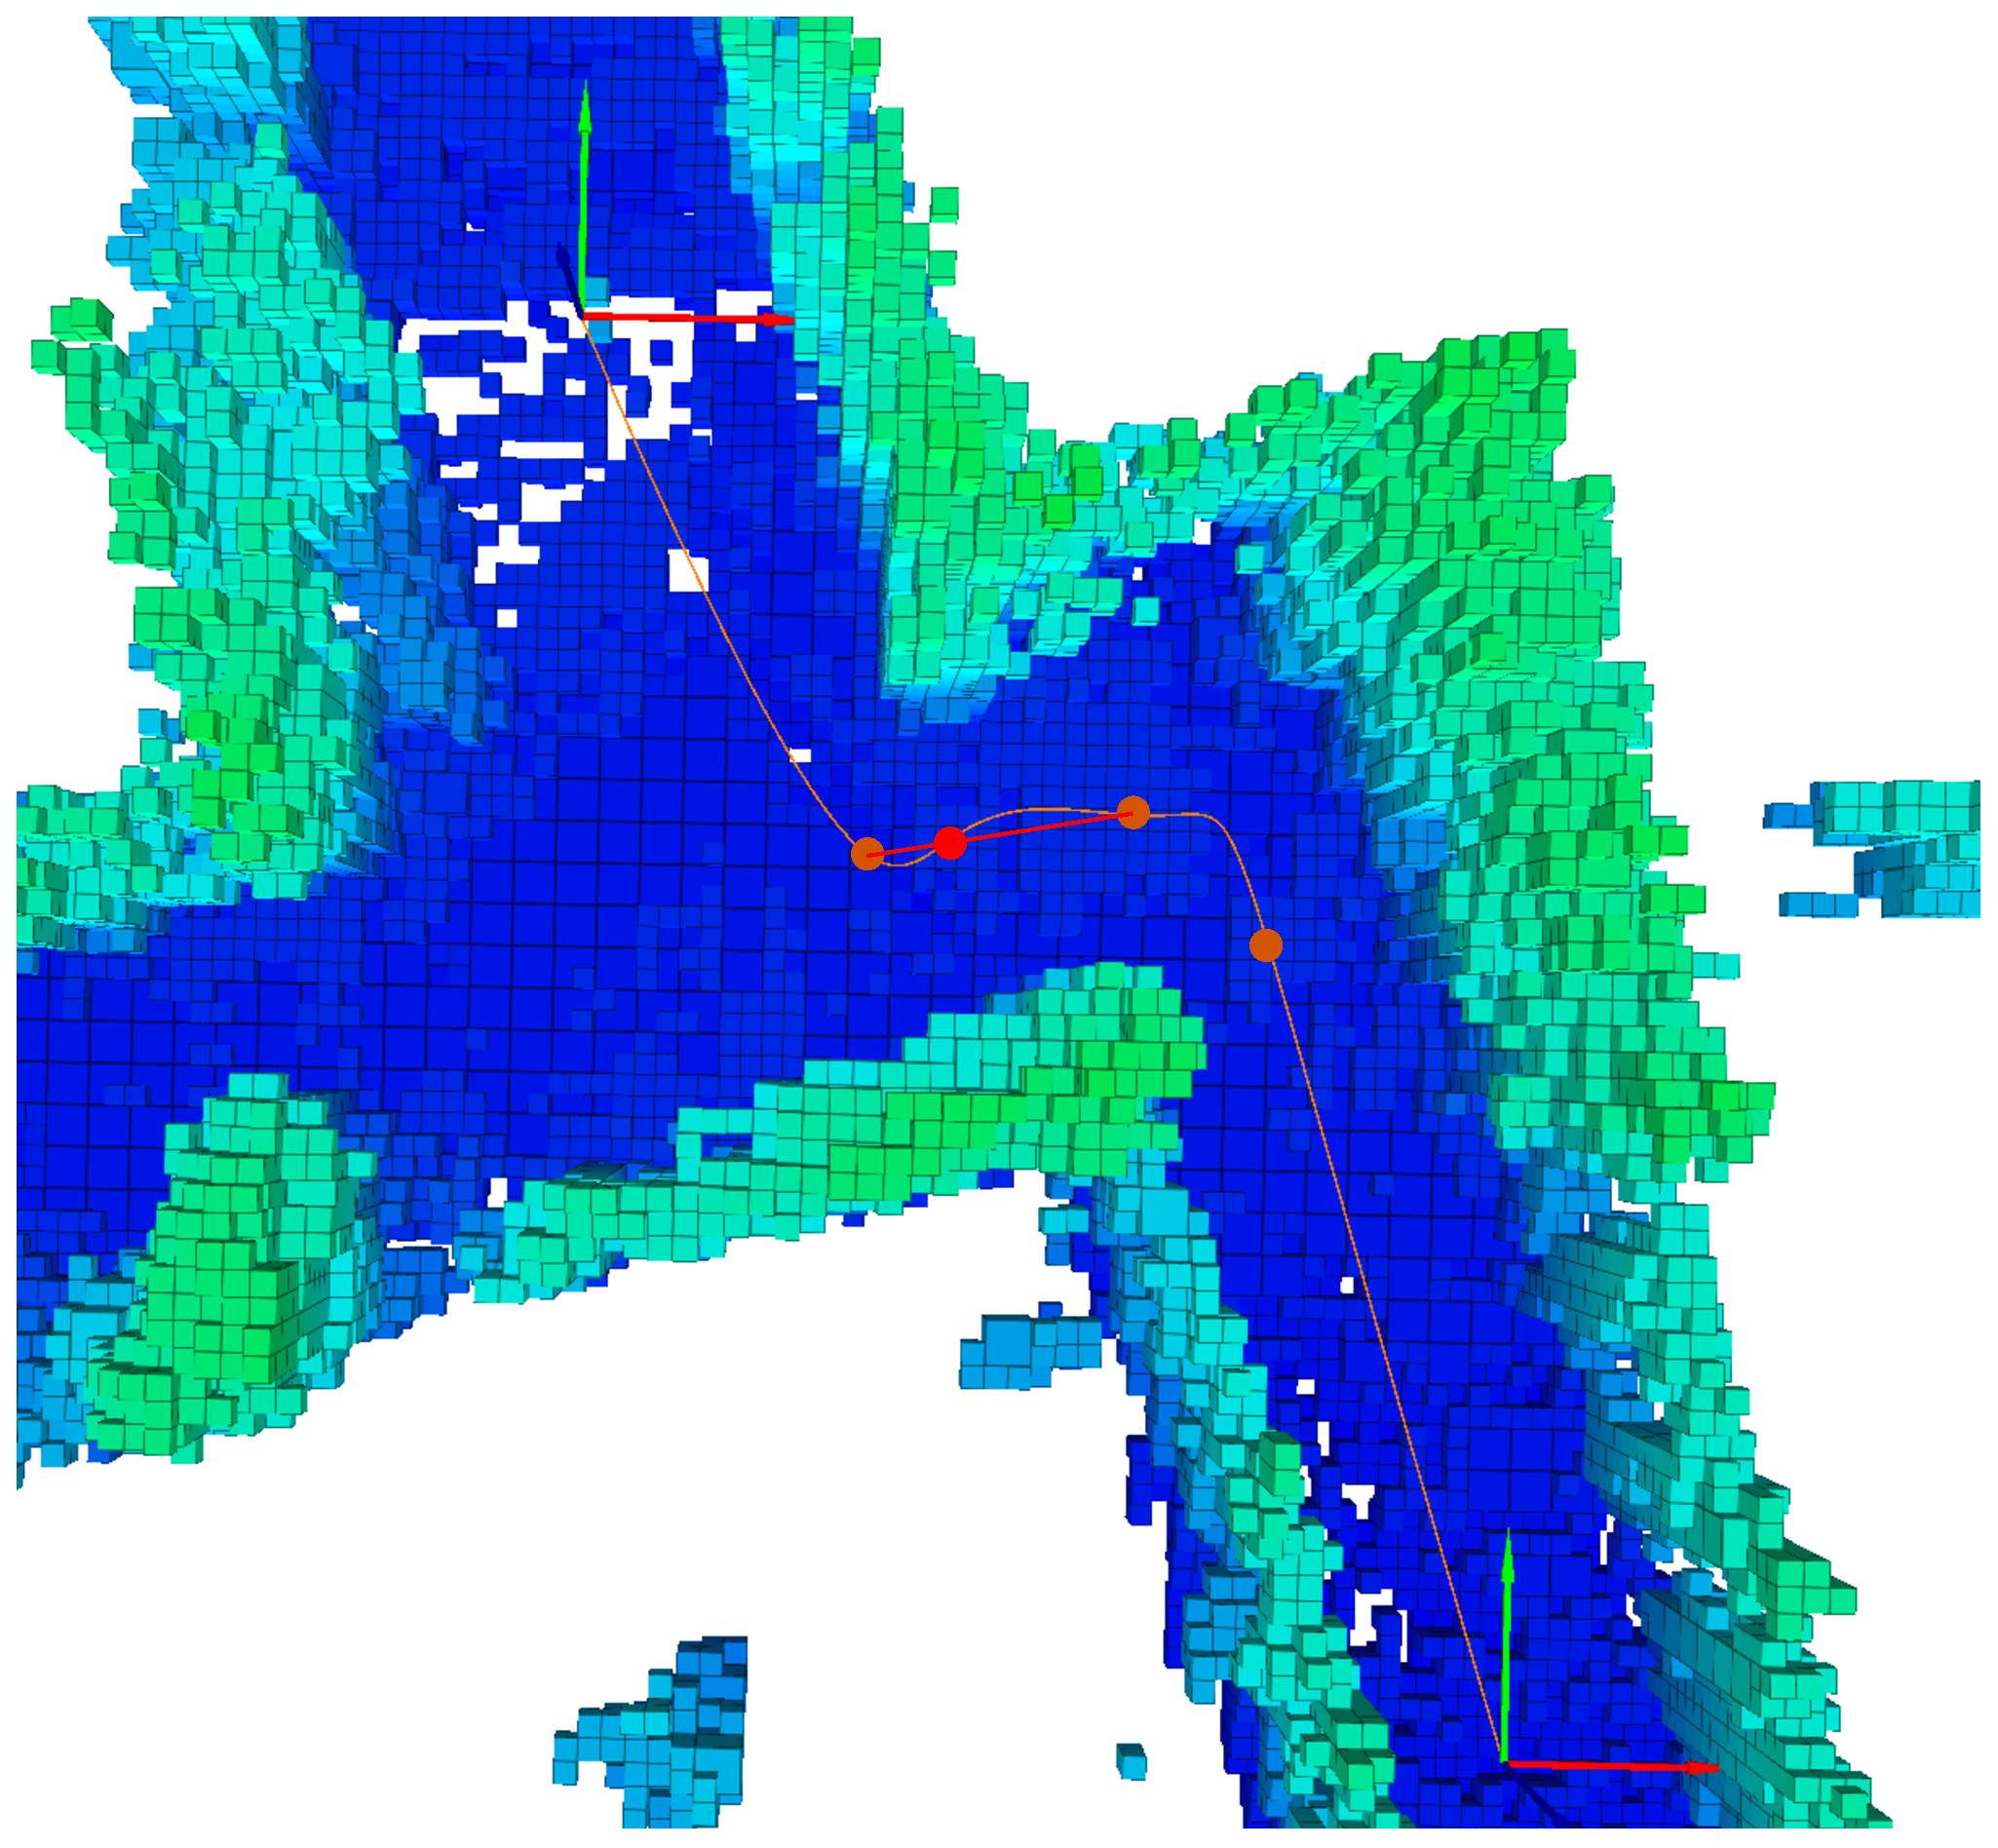
\includegraphics[trim = 45mm 0mm 35mm 5mm, clip,width=0.8\textwidth]{pics/extensionBLongPred.eps}
   \caption{Polynomial trajectory after a vertex extension, whereas the new vertex is represented by a red dot. The red line is not part of the trajectory but depicts the straight line connection of this segment.}
\label{pic:RRTstep3}
\end{figure}


To get an idea in which part of the trajectory the collision takes place, the length of the trajectory from the start of the segment to the collision is compared to the total trajectory length in this segment. This ratio is then mapped to the straight line solution and the additional vertex is placed. 
As explained in section \ref{sec:bbx}, the trajectory is in collision as soon as there is any obstacle inside the bounding box. Applied to the trajectory in figure \ref{pic:RRTstepTwo} this means that the collision is detected in the first half of the second segment before the trajectory itself proceeds through the wall of the hallway. Hence, the new vertex in figure \ref{pic:RRTstep3} is closer to the start of the second segment than to the end.



%\begin{figure}[h]
%   \centering
%   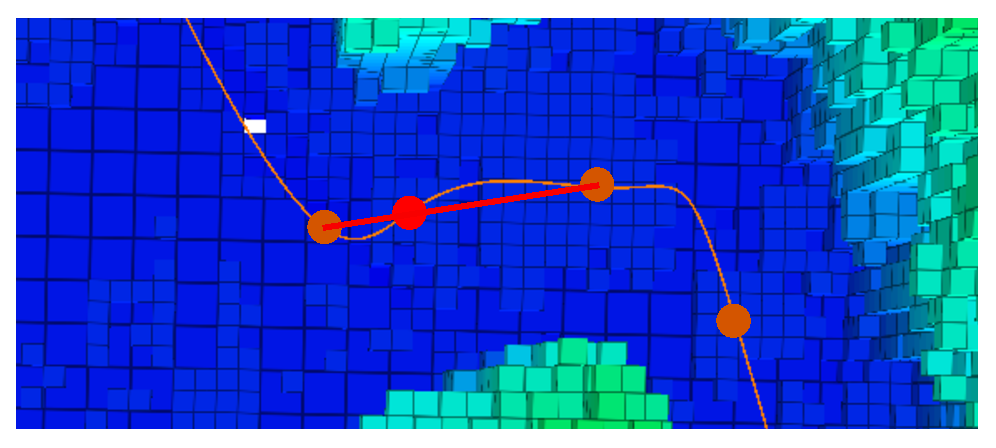
\includegraphics[width=1\textwidth]{pics/extensionBLongPredline.eps}
%   \caption{Ein Bild.}
%\end{figure}



\subsubsection{4. Perform a nonlinear optimization on the collision-free trajectory}

Using the trajectory depicted in figure \ref{pic:RRTstep3} as initial values a nonlinear optimization is performed. The optimized trajectory is depicted in figure \ref{pic:RRTstep4}. \newline


As mentioned in section \ref{sec:pathway}, the pathway of a snap minimized trajectory is mainly determined by the ratio of the segment times. Since the the ratio of the segment times of the trajectory in figure \ref{pic:RRTstep3} is not optimal the pathway contains unnecessary detours. \newline
After the nonlinear optimization, which includes an implicit optimization of the ratio of the segment times, the pathway is smoother and more suitable for a dynamic UAV flight.


\begin{figure}[h]
   \centering
   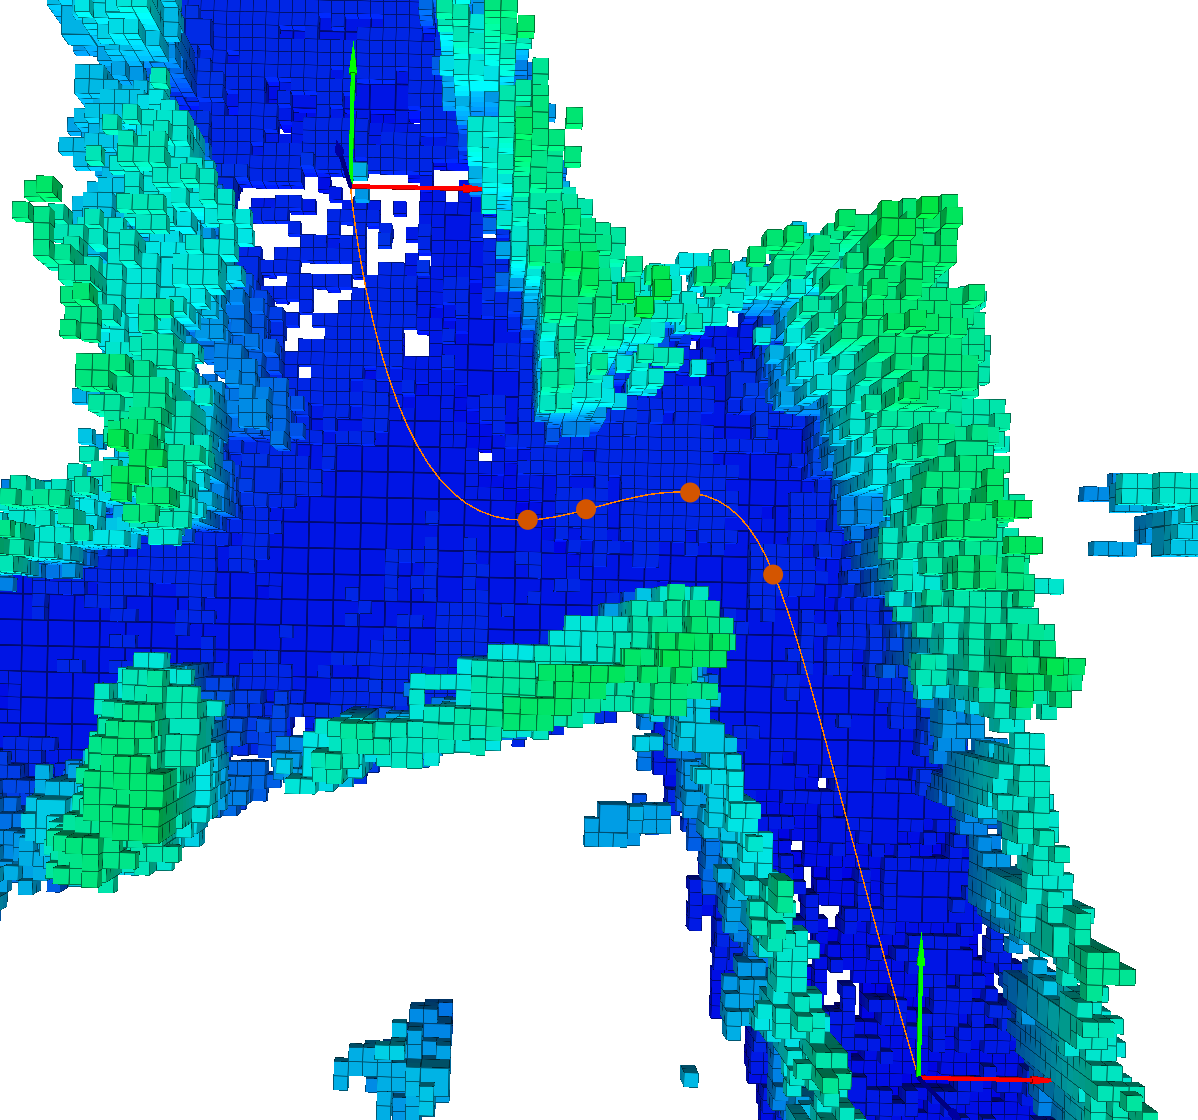
\includegraphics[trim = 60mm 0mm 35mm 0mm, clip,width=0.8\textwidth]{pics/extensionCLongP.png}
   \caption{The optimized trajectory with 5 segments.}
\label{pic:RRTstep4}
\end{figure}

\subsubsection{5. If the optimized solution is in collision, extend the existing vertices by a vertex located on the straight line solution and restart the nonlinear optimization. Repeat this step until the optimized trajectory is collision-free}
In this example the optimized trajectory is collision free without any further vertex extensions. Since the optimization smooths the trajectory but does not change the pathway of the trajectory completely, this is the general case. \newline

Nevertheless, if the optimized trajectory is in collision the vertex extension is equivalent to the procedure depicted in figure \ref{pic:RRTstep3}.

\subsection{Enlargement of the Bounding Box}\label{sec:enlargementBBX}

The initial trajectory passing through the vertices of the RRT* solution can be in collision although the straight line solution is collision free. This scenario is depicted in figure \ref{pic:RRTstepTwo}. \newline

As demonstrated, the collision can be bypassed by a vertex extension. But an additional vertex means additional optimization variables (endpoint derivatives and segment times). Thus not only the nonlinear optimization takes longer but the trajectory is more restricted and looses the possibility of more efficient and dynamical maneuvers.  \newline

Regarding the drawbacks listed above, it is preferable to avoid the necessity of a vertex extension. Therefore the bounding box is enlarged during the RRT* algorithm and then reduced to its original size for the trajectory planning. The resulting enlarged security corridor reduces the possibility of a collision in the initial trajectory. This enlargement of the bounding box can not be arbitrary high since the RRT* algorithm would no longer be able to find any solution through a densely packed environment if the bounding box for the straight line solution is to high. \newline

In this master thesis the individual dimensions of the bounding box are enlarged by $20\%$ for the straight line solution. This range reduces the necessity of a vertex extension but still enables the RRT* algorithm to find a solution through a densely packed environment.
%
%As a consequence, the factor of enlarging the bounding box for the straight line solution is a trade of. A large bounding box generally obviates the necessity of vertex extensions

\section{RRT* Replanning}\label{sec:replanningPassages}

It may happen that the straight line solution in a specific segment is very unsuitable to convert into a polynomial solution. In this case, this specific segment is still in collision after several vertex extensions. If so, it is reasonable to do a RRT* straight line replanning of this segment. Due to the randomness of the RRT* algorithm, the straight line solution will change. \newline

Please be aware that if a vertex extension is performed and this leads to a collision in a different part of the trajectory but the segment which was in collision in the initial solution is now collision free, no RRT* replanning is executed. \newline

Figure \ref{pic:vertexExtensionRRT} is a schematic depiction of an initial polynomial solution with 4 segments. The vertices are numbered and illustrated as dots initiating with the start vertex (vertex 0) on top. 
\begin{figure}[H]
   \centering
   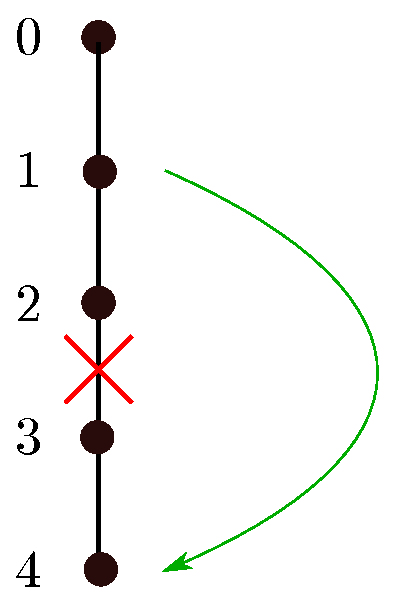
\includegraphics[width=0.2\textwidth]{pics/vertexExtensionRRT.eps}
   \caption{Schematic depiction of a initial polynomial solution with 4 segments. There is a collision in the third segment, marked as red cross. The replanning takes place between vertex 1 and vertex 4.}
   \label{pic:vertexExtensionRRT}
\end{figure}

In this example, the collision is in the third segment (i.e. between vertex 2 and vertex 3). If this collision, marked by the red cross, can not be eliminated with multiple vertex extension, a RRT* straight line replanning makes sense. In other words, vertex 2 and vertex 3 should be relocated. 

In order to achieve this, vertex 1 is used as the start vertex and vertex 4 is used as the goal vertex of a new RRT* straight line solution. This replanning is illustrated with a green arrow. As mentioned, the randomness of the RRT* algorithm leads to a new solution between vertex 1 and vertex 4.





\subsection{Threshold for the RRT* Replanning}\label{sec:RRTreplanning}

RRT* replanning requires an user-specified threshold which defines after how many vertex extension a segment is considered a difficult segment. In this master thesis, the RRT* replanning is triggered after one unsuccessful vertex extensions.\newline

Since one cycle of vertex extension defines a new vertex in every segment which is in collision, it is not trivial to find the difficult segment in the initial solution.

\begin{figure}[H]
   \centering
   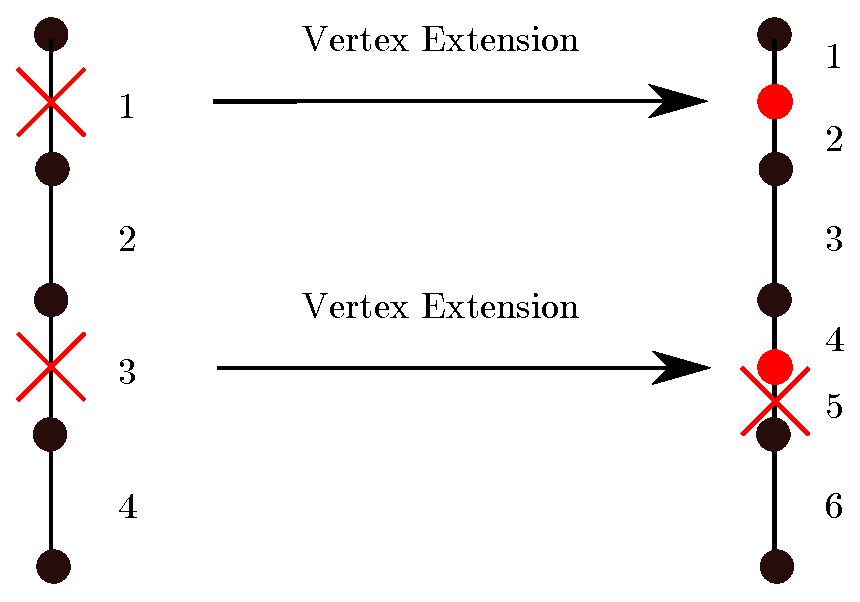
\includegraphics[width=0.6\textwidth]{pics/recogniseSegment.eps}
   \caption{One cycle of vertex extension. In the initial solution on the left-hand side of the figure there is a collision in segment 1 and segment 3. After one cycle of vertex extension there are 6 segments. }
   \label{pic:recognise}
\end{figure}

In figure \ref{pic:recognise} the segments are numbered. The left-hand side depicts the initial solution with a collision in segment 1 and segment 3. For both segments, a new vertex is added as illustrated as a red dot in the right-hand side of figure \ref{pic:recognise}. To find the difficult segment, 4 pairs of numbers have to be stored. The pairs consists of the initial segment which is in collision and of the corresponding segment after the vertex extension. \newline

The four pairs resulting from figure \ref{pic:recognise} are listed in the following table:

\begin{table}[H] 
\begin{center}
    \begin{tabular}{| c | c | c | }
    \hline
    Pair & Initial Segment & Extended Segment\\ \hline
   i) & 1 & 1 \\ \hline
   ii) & 1 & 2\\ \hline
   iii) & 3 & 4\\ \hline
   iv) & 3 & 5\\
    \hline
    \end{tabular}
    \caption{Four pairs of numbers, representing possible difficult segments. Every initial segment is connected to two extended segments.}
    \label{tab:pairsOfNumbers}
\end{center}
\end{table}

In the example depicted in figure \ref{pic:recognise} there is a collision in segment 5 after the vertex extension. 
Therefore, pair iv) gets significant and segment 3 (from the initial straight line solution) is exposed as a difficult segment. Once the difficult segment is located, the RRT* replanning can be performed as illustrated in figure \ref{pic:vertexExtensionRRT}.

\subsection{Store the Best Initial Solution}

A difficult segment in the initial solution does not mean that is impossible to find a collision free polynomial trajectory. Meaning the polynomial solution which is still in collision after one cycle of vertex extension, depicted in the right-hand side of figure \ref{pic:recognise}, can be collision-free after additional vertex extensions. If possible, the initial RRT* straight line solution is converted into a collision free polynomial trajectory with multiple vertex extensions and the polynomial trajectory and the corresponding total cost of the trajectory is stored. \newline

Not until then the RRT* replanning is performed. The difficult section of the original straight line solution is then replaced by the replanned section and a polynomial trajectory passing trough the vertices is computed. The new trajectory on his part can be in collision and vertex extensions have to be performed until the trajectory is collision-free. Once the trajectory is collision-free, the total cost of the new trajectory is compared to the total cost of the first trajectory and the one with the lower cost is used for the nonlinear optimization.

\section{Overall Implementation}

All the features which are discussed so far will be combined to the final implementation.  Figure \ref{pic:overall} is simplified but a clearly arranged schematic depiction of the final implementation:
%
%\begin{figure}[H]
%   \centering
%   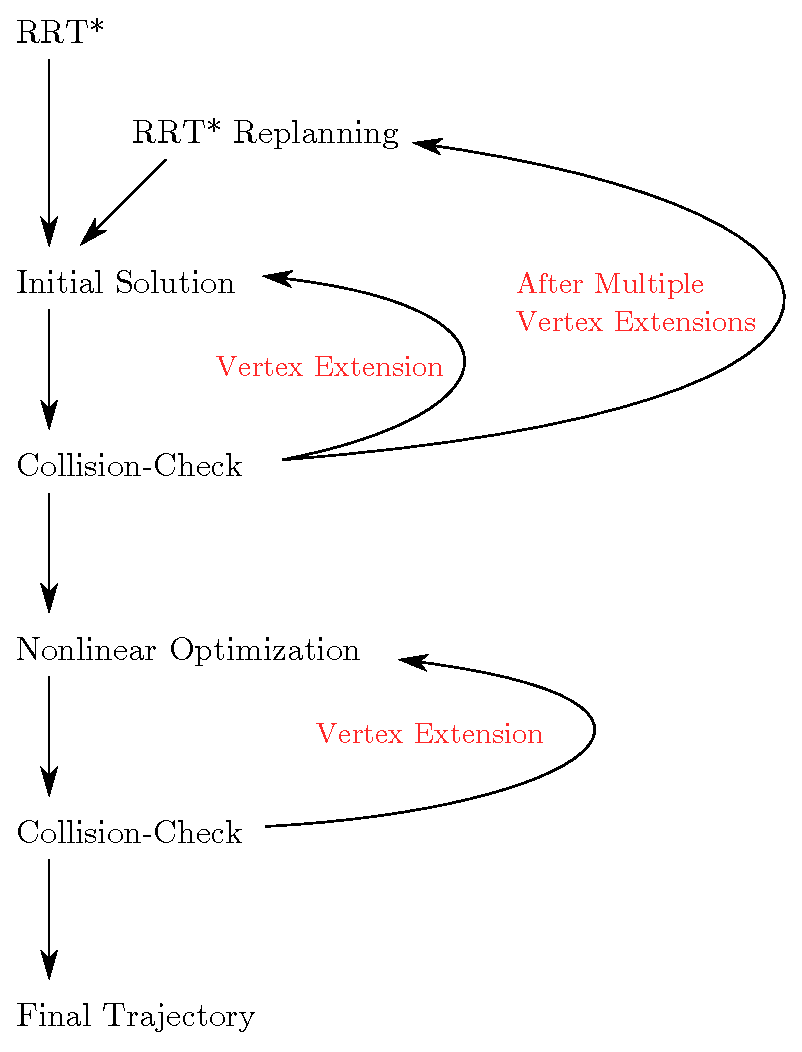
\includegraphics[width=0.6\textwidth]{pics/overall.eps}
%   \caption{Schematic depiction of the final implementation of the path planning algorithm.}
%   \label{pic:overall}
%\end{figure}

\begin{figure}[H]
   \centering
   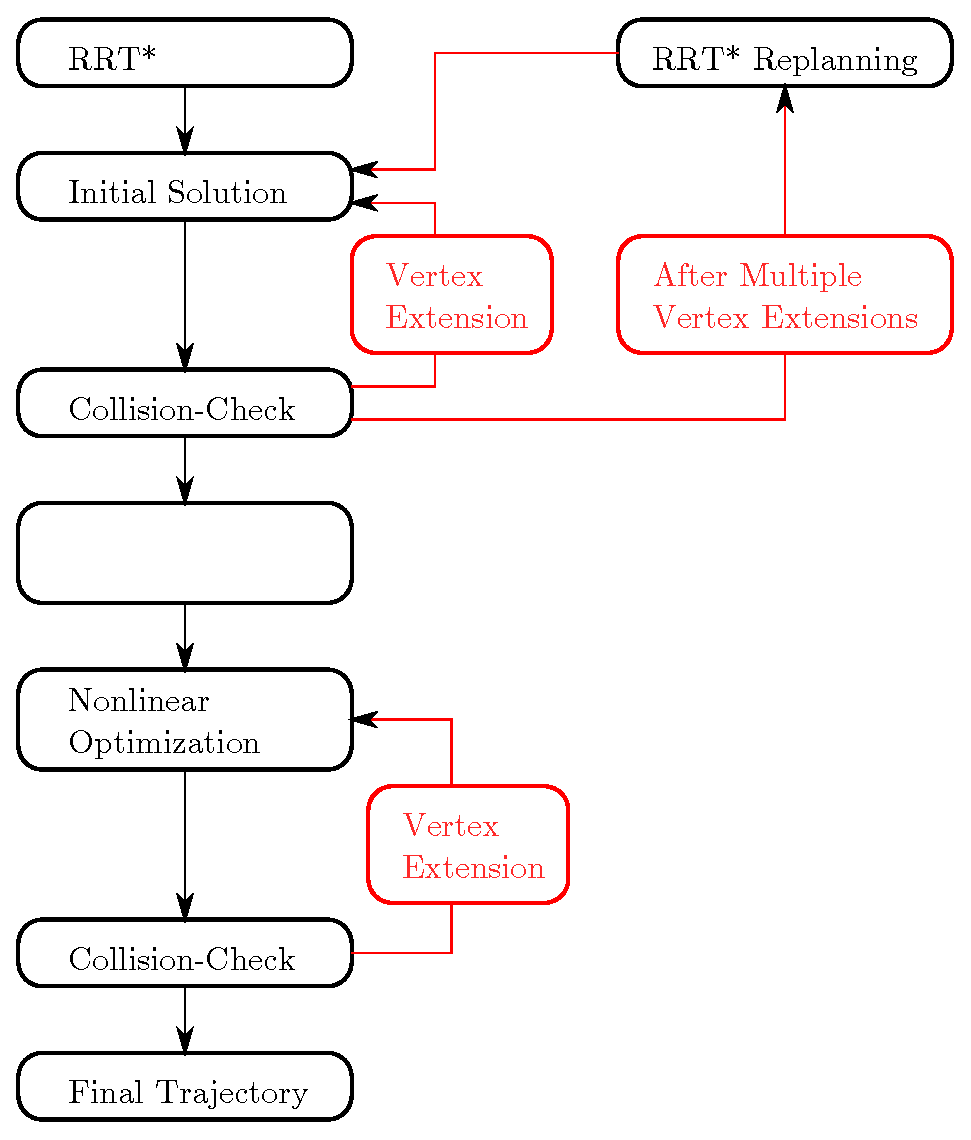
\includegraphics[width=0.66\textwidth]{pics/overall2.eps}
   \caption{Schematic depiction of the final implementation of the path planning algorithm.}
   \label{pic:overall}
\end{figure}

The most important user-specified parameters of this final implementation are discussed in the next section.






\section{Robot Operating System}

The whole program is built using the \href{http://www.ros.org/}{Robot Operating System (ROS)} \cite{ROS}. To be exact, it is built as a ROS node. A node is a process that performs computation. Nodes are combined together into a graph and communicate with one another using streaming topics, services, and the Parameter Server. A very powerful feature of ROS is "Dynamic Reconfigure". This tool allows the user to change parameters during runtime. Runtime is the period of time when a program is running. It begins when a program is opened (or executed) and ends with the program is quit or closed.

\subsection{Dynamic Reconfigure}\label{sec:dynamicRec}

In this master thesis, several imported parameters are modifiable by Dynamic Reconfigure. Mainly, two of them determine the performance of the RRT* algorithm:

\begin{itemize}
  \item $\gamma$
  \item $endRRT$
\end{itemize}

The $\gamma$ parameter determines the amount of rewiring and is described in detail in section \ref{sec:Rewiring}. $endRRT$ defines how many additional RRT* iteration are performed after a collision-free straight line connection is found. Thus, $endRRT = 2000$ leads to 2000 additional iterations in which the algorithm can improve the straight lines solution via rewiring. \newline

The next two parameters which are included into Dynamic Reconfigure are used to modify NLopt:

\begin{itemize}
  \item $J_{rel}$
  \item $k_T$
\end{itemize}


$J_{rel}$ is defined in section \ref{sec:NLopt} and is an ending criteria for NLopt. The weighting factor $k_T$ is defined in equation \ref{equ:total_cost} in section \ref{sec:penalty} and specifies the aggressiveness of a trajectory. \newline

The next modifiable parameter concerns the RRT* replanning. As explained in section \ref{sec:replanningPassages}, a RRT* replanning is beneficial if there are difficult passages in the initial straight line solution. It may happen, that the straight line solution with the replanned segments still has difficult passages. 

\begin{itemize}
  \item $maxReplanning$
\end{itemize}

$maxReplanning$ defines the max. number of RRT* replannings. After this number of replannings, the optimization starts with the best solution so fare. If no collision-free solution has been found, the complete RRT* planning starts again. \newline

The last modifiable parameter, a Boolean parameter (either "true" or "false"), affects the start vertex of a trajectory:

\begin{itemize}
  \item $currentPose$
\end{itemize}


$currentPose$ defines if the start vertex is either manually chosen or the actual current pose of the UAV. In this master thesis, the current pose is provided by \href{http://www.vicon.com/}{Vicon} \cite{Vicon}, a powerful object tracking solution providing unrivaled data accuracy for integration in to 3D applications. If $currentPose$ is set to "true" the current pose provided by Vicon is used as the start vertex.







%\subsection{Multiple Vertex Extension}

%\begin{figure}[h]
%   \centering
%   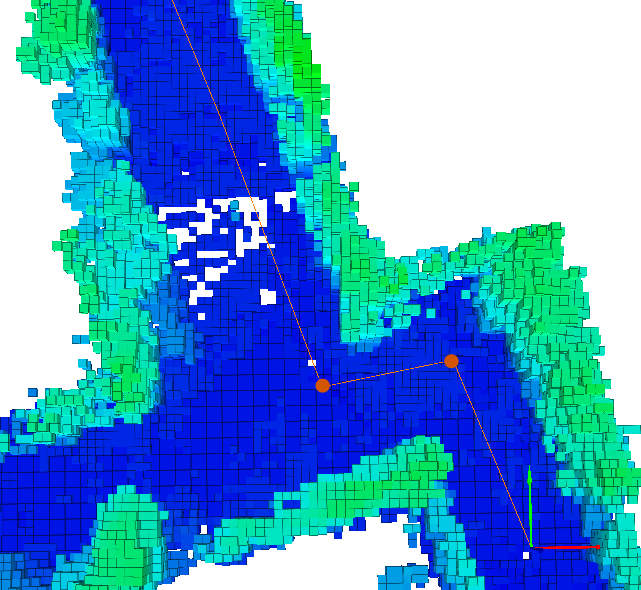
\includegraphics[width=1\textwidth]{pics/1LongP.png}
%   \caption{Ein Bild.}
%\end{figure}
%
%
%
%\begin{figure}[h]
%   \centering
%   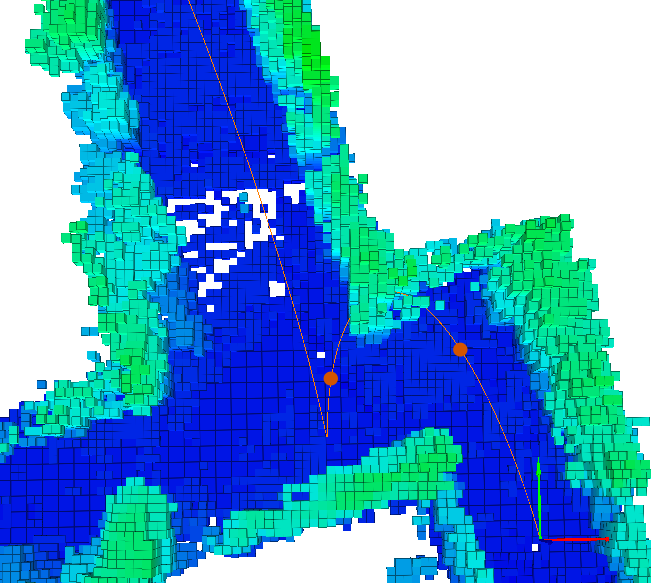
\includegraphics[width=1\textwidth]{pics/1aLongP.png}
%   \caption{Ein Bild.}
%\end{figure}
%
%
%\begin{figure}[h]
%   \centering
%   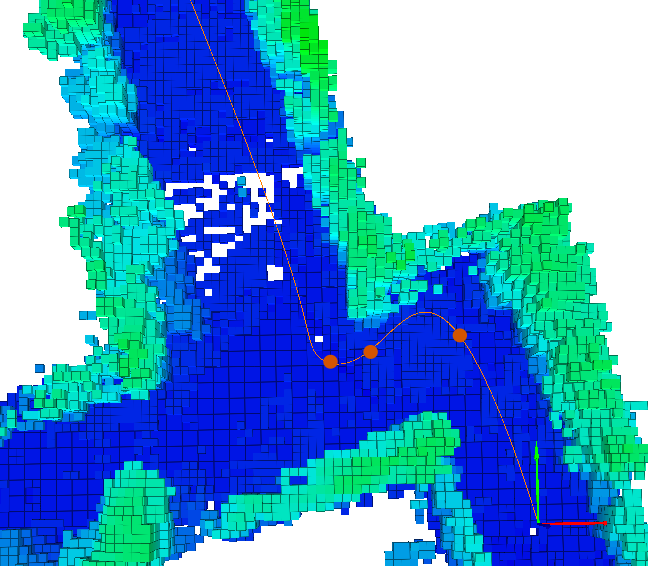
\includegraphics[width=1\textwidth]{pics/1bLongP.png}
%   \caption{Ein Bild.}
%\end{figure}
%
%\begin{figure}[h]
%   \centering
%   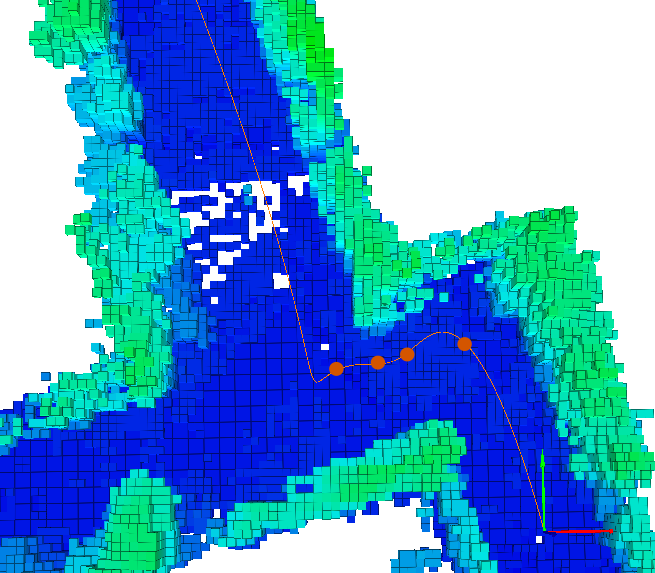
\includegraphics[width=1\textwidth]{pics/1cLongP.png}
%   \caption{Ein Bild.}
%\end{figure}
%
%\begin{figure}[h]
%   \centering
%   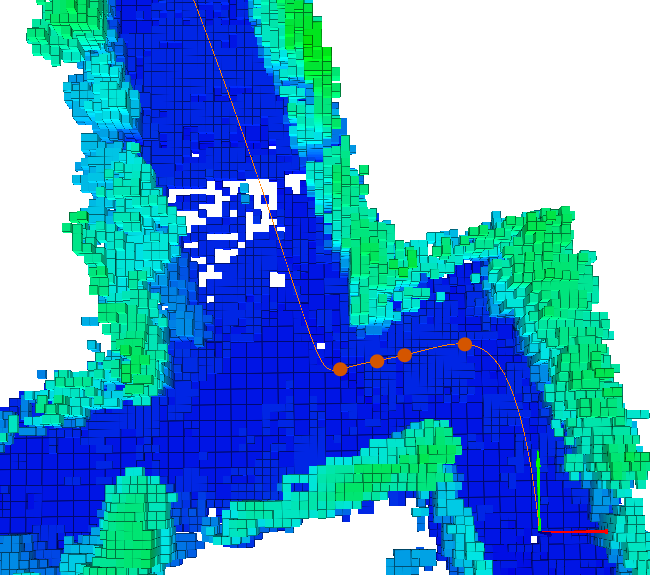
\includegraphics[width=1\textwidth]{pics/1dLongP.png}
%   \caption{Ein Bild.}
%\end{figure}
%
%


 \cleardoublepage
  \chapter{Results}\label{chap:Results}


\section{Performance of the RRT* Algorithm}\label{sec:performanceRRT}

In this master thesis, the performance of the RRT* algorithm itself was not improved but the parameters were tuned to serve the nonlinear optimization in an optimal manner.\newline
As mentioned in section \ref{sec:RRTstar}, the calculation time of the RRT* algorithm is mainly defined by the "rewiring" and therefore by the user specified parameter $\gamma$ (used in equation \ref{equ:ballradius}). A good straight line solution, whereas good means a small length of the straight line solution, does not necessarily lead to a good polynomial trajectory. The influence of the user specified parameter $\gamma$ on the final trajectory and the corresponding calculation time is evaluated in this section. \newline
Please call to mind that a small $\gamma$ parameter means little rewiring and a big $\gamma$ parameter means lots of rewiring. The impact of the $\gamma$ parameter can be looked up in figure \ref{pic:smallGamma} and figure \ref{pic:smallBBX}.\newline

\begin{figure}[H]
   \centering
   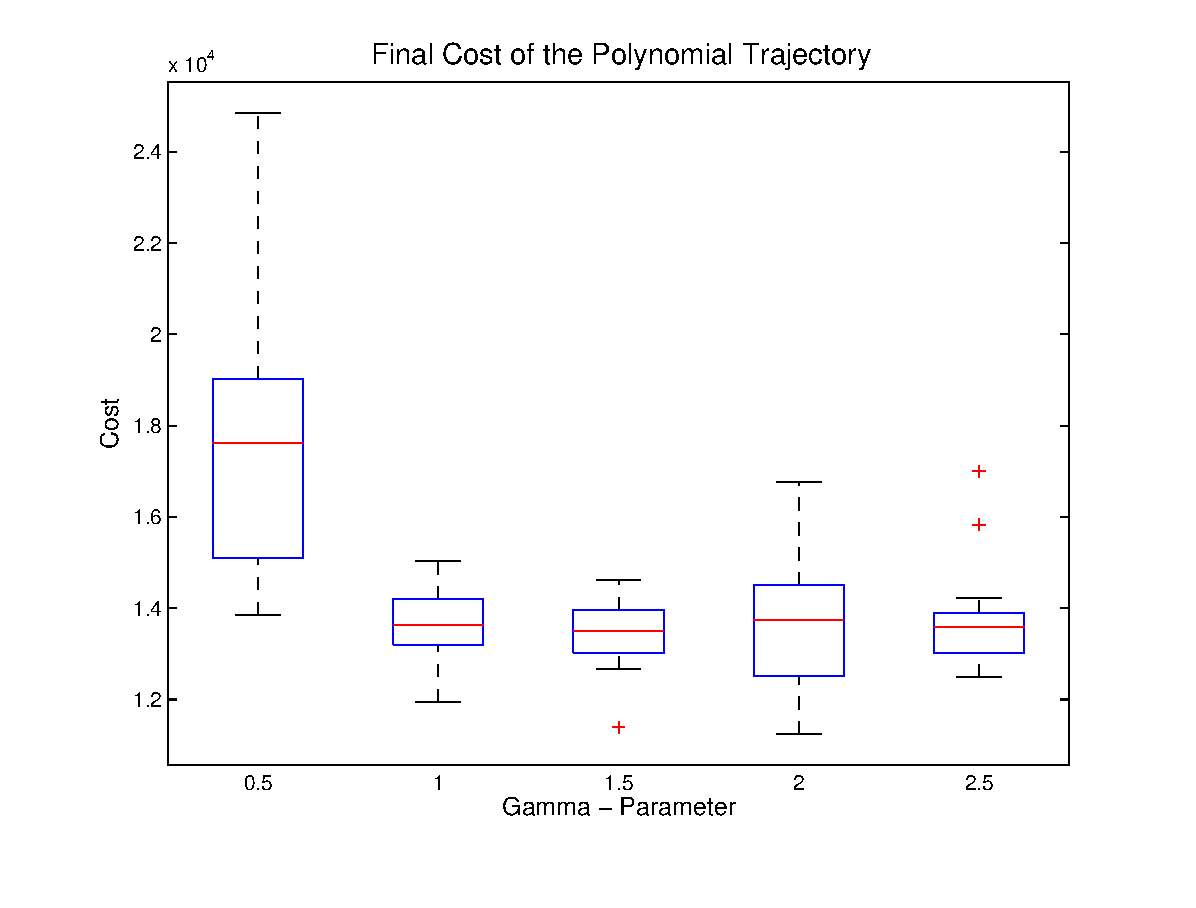
\includegraphics[trim = 14mm 10mm 15mm 0mm,clip,width=0.8\textwidth]{pics/boxplot1.eps}
   \caption{The $x$-axis depicts different $\gamma$ parameters and the $y$-axis depicts the final cost of the polynomial trajectory. The red mark illustrates the median. }
   \label{pic:boxplot}
\end{figure}

Figure \ref{pic:boxplot} depicts the boxplot for different $\gamma$ parameters. Each dataset consists of 15 measurements. On each box, the central mark is the median, the edges of the box are the 25th and 75th percentiles, the whiskers extend to the most extreme
datapoints the algorithm considers to be not outliers, and the outliers are plotted individually. \newline





It becomes apparent that the small amount of rewiring associated with $\gamma = 0.5$ is to little to obtain a good polynomial trajectory. The 4 remaining datasets have a similar performance in terms of the final trajectory cost. \newline

The total computational times for the five different $\gamma$ parameters are depicted in figure \ref{pic:boxplot_time}. The total computational time is the combined duration of the RRT* algorithm and the nonlinear optimization. In contrast to the final cost, the total computational times for $\gamma = 1 $, $\gamma = 1.5$, $\gamma = 2$ and $\gamma = 2.5$ are distinct. 

\begin{figure}[h]
   \centering
   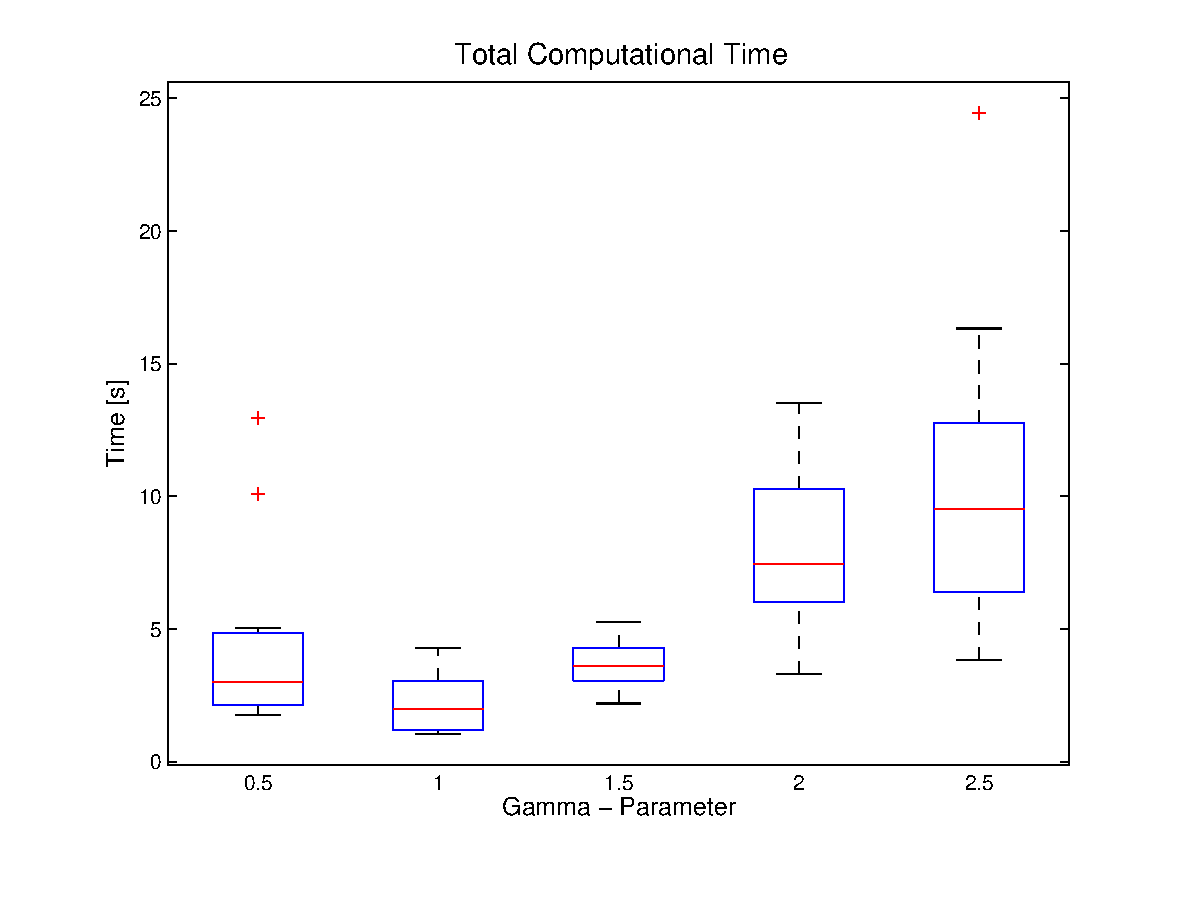
\includegraphics[trim = 14mm 10mm 15mm 0mm,clip,width=0.8\textwidth]{pics/boxplot_time.eps}
   \caption{The $x$-axis depicts different $\gamma$ parameters and the $y$-axis depicts the total computational time. The red mark illustrates the median.}
   \label{pic:boxplot_time}
\end{figure}

Figure \ref{pic:boxplot_time} shows that the computational time increases significant if $\gamma$ is larger than 1.5. This is simply because the RRT* algorithm needs more time for rewiring. Furthermore, $\gamma = 0.5$ (which is not a good choice sine the final cost is too high) has 2 outliers. In this 2 cases the straight line solution is not enough target-orientated and multible vertex extensions are required to obtain a collision-free trajectory. \newline

Combining the results from figure \ref{pic:boxplot} and figure \ref{pic:boxplot_time}, a $\gamma$ parameter in the range of 1 to 1.5 lead to the best performance.




\section{Performance of NLopt}

To test the performance of NLopt, a nonlinear optimization library, trajectories of different length were optimized. Figure \ref{pic:differentGoal} depicts a start vertex and 6 different goal vertices. The figure is in bird's eye perspective and shows a crossing of different hallways. The blue cells represents the floor and the green cells represents the walls. 
 In some of the hallways, there are objects blocking (part of) the way. This passages are tagged with "Bottleneck". Please note that other passages which may look like a bottleneck, such as the top right corner, are not blocked. The green boxes in this passage are part of the ceiling.

\begin{figure}[H]
   \centering
   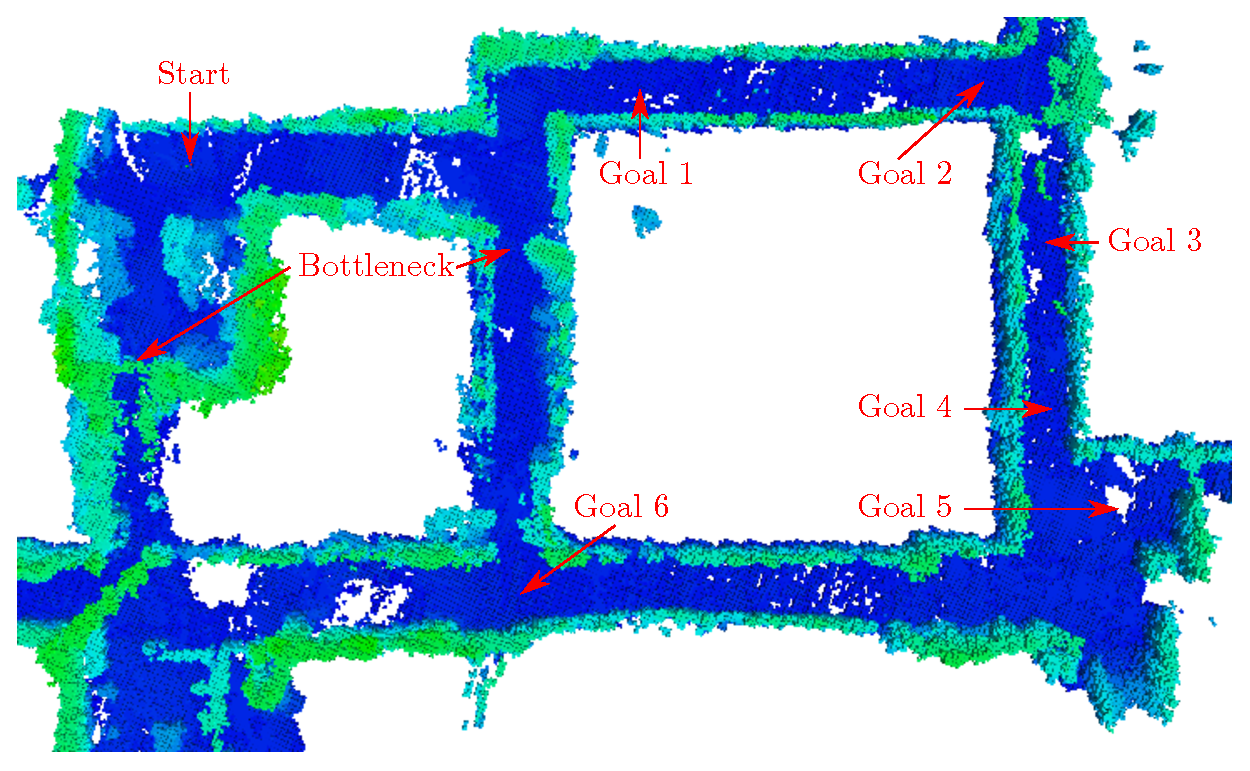
\includegraphics[trim = 0mm 15mm 0mm 0mm,clip,width=1\textwidth]{pics/ML4.eps}
   \caption{Bird's eye perspective on hallways in the "ML" building of the ETH Zurich. One start vertex and 6 different goal vertices are depicted}
   \label{pic:differentGoal}
\end{figure}

%\begin{figure}[h]
%   \centering
%   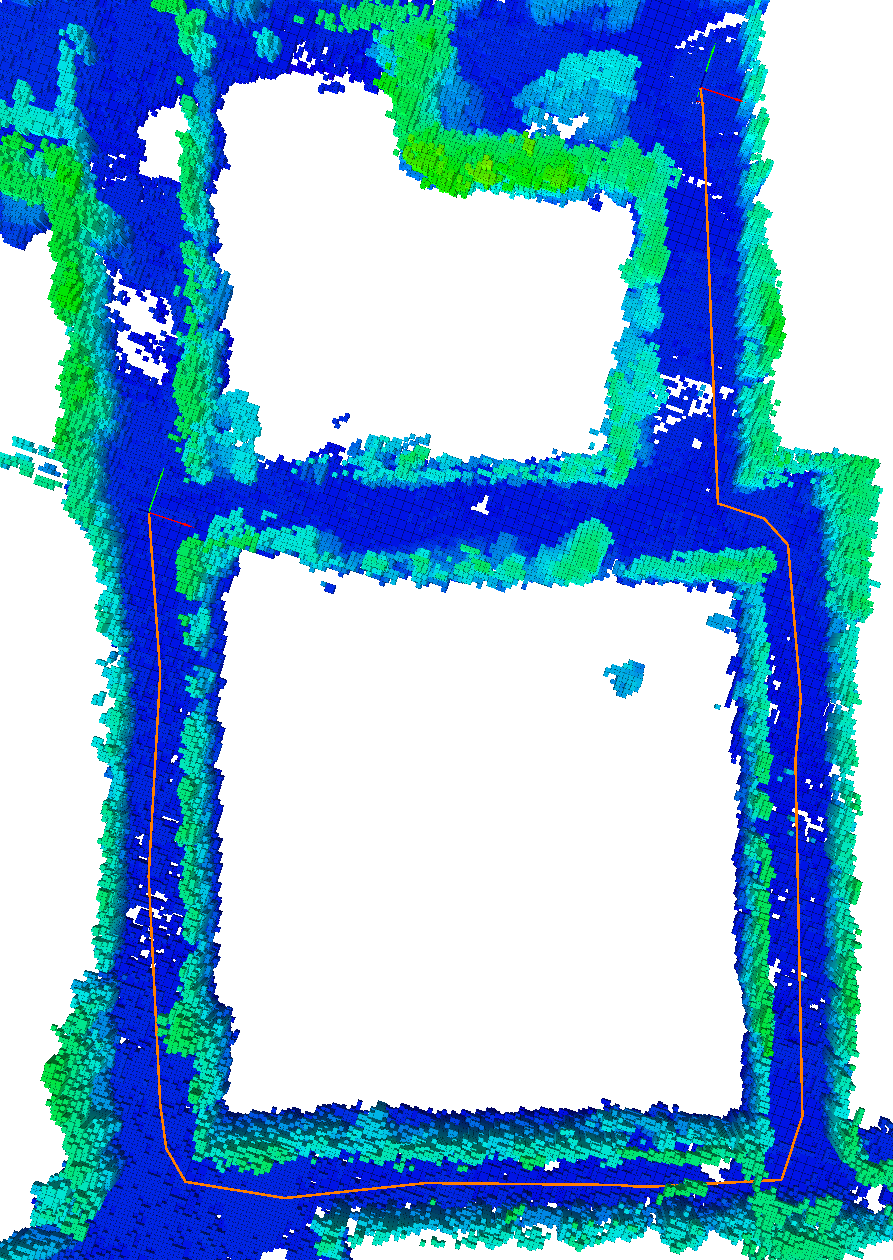
\includegraphics[width=0.5\textwidth]{pics/MapLine.png}
%   \caption{Ein Bild.}
%\end{figure}
%
%
%\begin{figure}[h]
%   \centering
%   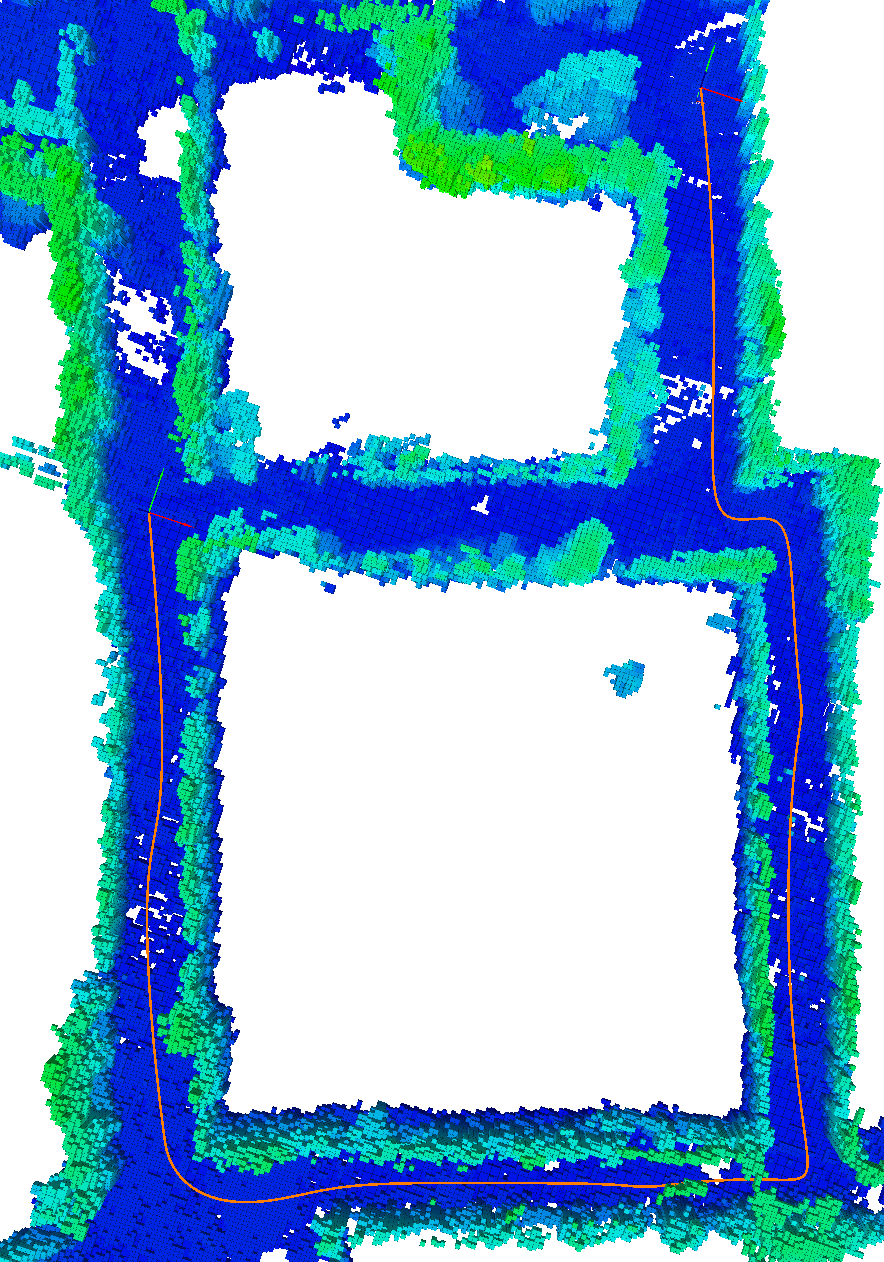
\includegraphics[width=0.5\textwidth]{pics/MapPoly.png}
%   \caption{Ein Bild.}
%\end{figure}

The bottleneck in the center of figure \ref{pic:differentGoal} gets significant for large bounding boxes. If the dimension of the bounding box are larger than $0.5m$ x $0.5m$ x $0.5m$ the trajectory is not able to pass the bottleneck. Hence, a trajectory with a large bounding box has to go all the way around to proceed from the start vertex to "Goal 6" as depicted in figure \ref{pic:Goal6}.


\begin{figure}[H]
   \centering
   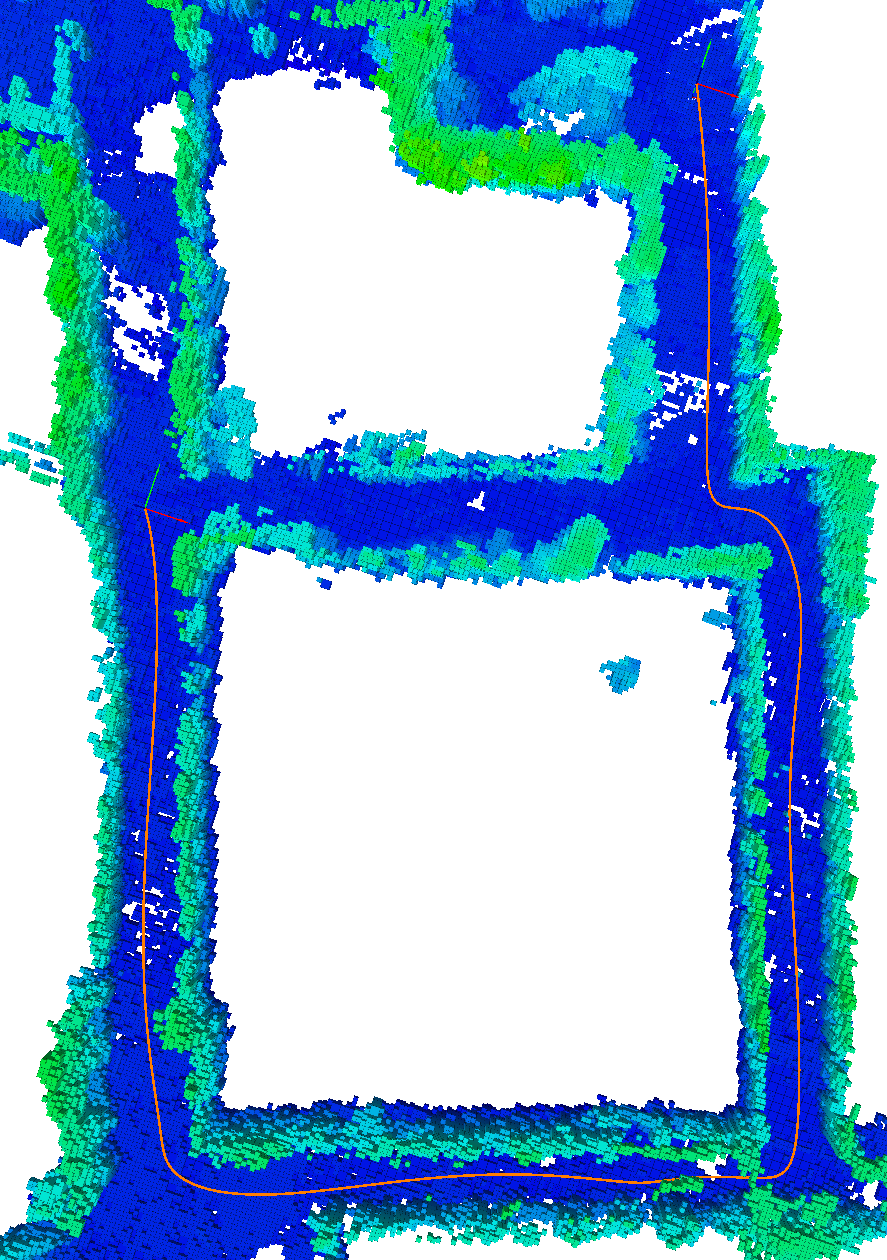
\includegraphics[angle=90,trim = 20mm 0mm 0mm 0mm,clip, width=1\textwidth]{pics/MapNlopt.png}
   \caption{Trajectory from the start vertex to "Goal 6". Due to the bottleneck in the hallway in the middle, the trajectory has to proceed all the way around.}
   \label{pic:Goal6}
\end{figure}

The trajectories from the start vertex to the 6 different goal vertices (depicted in figure \ref{pic:differentGoal}) are examined for number of segments and the duration of NLopt. The only ending criteria for NLopt was the relative criteria on the total cost $f_{rel} = 0.02$. 
In addition to the number of segments, the number of corresponding optimization variables (endpoint derivatives $d_p$ and segment times $T_i$) are calculated. For all the "free" vertices (which are neither the start nor the goal vertex) there are 12 optimization variables, namely the velocity, the acceleration, the jerk and the snap in the 3 dimensions. Furthermore, the segment times are optimization variables. \newline

Since the number of free vertices is the number of segment $n_{seg}$ minus 1, the equation for the number of optimization variables $n_{var}$ is:

\begin{equation}
n_{var} = (n_{seg} - 1)\cdot 12 + n_{seg}
\label{equ:numberOfSeg}
\end{equation}

The results for the 6 different goal vertices are listed in the following table:


\begin{table}[H] 
\begin{center}
    \begin{tabular}{| c | c | c | c | }
    \hline
    Goal Vertex & Segments & Optimization Variables & Optimization Time\\ \hline
   Goal 1 & 5 & 53 & $1.15s$\\ \hline
  Goal 2 & 8 & 92 & $2.94s$\\ \hline
   Goal 3 & 11 & 131 & $7.80s$\\ \hline
Goal 4 & 15 & 183& $42.96s$\\ \hline
Goal 5 & 19 & 235& $93.08s$\\ \hline
   Goal 6& 20 & 248 & $347.62s$\\
    \hline
    \end{tabular}
    \caption{The number of segments of the collision free polynomial solution and the corresponding number of optimization variables. The time needed by NLopt with the ending criteria $f_{rel} = 0.02$.}
    \label{tab:MLoptimizationTime}
\end{center}
\end{table}

Table \ref{tab:MLoptimizationTime} shows that the optimization time (i.e. the duration of the NLopt algorithm) increases significant for a large amount of optimization variables. Comparing the result of "Goal 5" to "Goal 6" it becomes clear, that the number of optimization variables is not the only factor which determines the optimization time. If the optimization values of the initial solution are close to the global minimum of the cost function, the optimization takes less time and vice versa. Still, the number of optimization variables is the main factor. \newline

Please note that the RRT* algorithm was only executed once for every goal vertex. Due to the randomness of the RRT* algorithm, the number of segments could change for unchanged start and goal vertices.\newline



\section{Reduction of the Optimization Variables}

The results in table \ref{tab:MLoptimizationTime} have shown, that the performance of NLopt decreases with a large amount of optimization variables. In cases where the optimization times is significant (i.e. online planning) the number of optimization parameters has to be reduced. The benefits and the drawbacks of a cost function with fewer optimization variables is discussed in the next section. \newpage

\subsection{Cost Function Without Endpoint Derivatives}

To call to mind, the cost function for the nonlinear optimization is 

\begin{equation}
J_{total} =
\begin{bmatrix}
   d_f \\
  d_p
\end{bmatrix}^T
\begin{bmatrix}
   R_{ff} & R_{fp} \\
  R_{pf} & R_{pp}
\end{bmatrix}
\begin{bmatrix}
   d_f \\
  d_p
\end{bmatrix}
+ k_T \cdot \sum_{i=1}^N T_i
\label{equ:total_cost_Result}
\end{equation}

where the optimization variables are the segment times $T_i$ and the unspecified endpoint derivatives $d_p$. $k_T$ is a user specified weighting factor and $d_f$ is the vector containing the fixed endpoint derivatives. The 4 sub-matrices of $R$ are containing the quadratic snap rearranged according to the fixed and unspecified endpoint derivatives. \newline
As discussed in section \ref{sec:nonlinearopt}, the optimum of this cost function can not be found analytically but with a nonlinear optimization. Only the snap minimized solution of a trajectory with fixed segment times can be computed analytically according to 



\begin{equation}
d_p^* = - R_{pp}^{-1} \cdot R_{fp}^T \cdot d_f
\label{equ:dpstar_Result}
\end{equation}

where the optimal unspecified endpoint derivatives  $d_p^*$ are a function of the fixed derivatives $d_f$ and two of the submatrices ($R_{pp}, R_{fp}$) of $R$. \newline

Since the endpoint derivatives $d_p$ can be found analytically once the segment times $T_i$ are known, $d_p$ can be excluded from the optimization variables. In other words, in every optimization steps the segment times are modified by NLopt. Then $d_p^* $ is computed with the current segment times and the total cost is calculated according to equation \ref{equ:total_cost_Result}. \newline

Recapitulating the new cost function:

\begin{itemize}
  \item The segment times $T_i$ are the only optimization variables.
  \item The optimal unspecified endpoint derivatives $d_p^*$ are computed analytically (equation \ref{equ:dpstar_Result}) every optimization step with the current segment times.
    \item The cost function (equation \ref{equ:total_cost_Result}) gets minimized.
\end{itemize}

\subsection{Comparison of the Analytical Solvers}

Before we can compare the performance of the approach with the full number of optimization variables (in the interests of simplification called approach A) to the approach with the reduced number of optimization variables (approach B) we have to examine the performance of the analytical solver which solves equation \ref{equ:dpstar_Result}.\newline

An analytical or linear solver is able to solve an single matrix equation:

\begin{equation}
A \cdot x = b
\label{equ:linearSolver}
\end{equation}


Indeed, equation \ref{equ:dpstar_Result} is a single matrix equation where $-R_{pp}$ is represented by $A$ and $x$ is the vector containing the optimization variables (i.e. $d_p$). Furthermore, $R_{fp}^T \cdot d_f$ can be taken together as vector $b$. \newline

In this master thesis, three different strategies have been implemented to solve equation \ref{equ:dpstar_Result}.
All of them are part of "Eigen". Eigen is a C++ template library for linear algebra: matrices, vectors, numerical solvers, and related algorithms. The definition of the implemented strategies can be found on the  \href{http://eigen.tuxfamily.org/index.php?title=Main_Page}{Eigen-homepage} \cite{Eigen}:

\newpage

\subsubsection{FullPivLU}

This class represents a $LU$ decomposition of any matrix, with complete pivoting: the matrix $A$ is decomposed as $A = PLUQ$ where $L$ is unit-lower-triangular, $U$ is upper-triangular, and $P$ and $Q$ are permutation matrices. This is a rank-revealing $LU$ decomposition. The eigenvalues (diagonal coefficients) of $U$ are sorted in such a way that any zeros are at the end. \newline

$FullPivLU$ is a very accurate technique but rather slow.

\subsubsection{HouseholderQR}

This class performs a $QR$ decomposition of a matrix $A$ into matrices $Q$ and $R$ such that $A = QR$ by using Householder transformations. Here, $Q$ a unitary matrix and $R$ an upper triangular matrix. The result is stored in a compact way compatible with $LAPACK$. Note that no pivoting is performed. This is not a rank-revealing decomposition.\newline

$HouseholderQR$ is a fast technique but in general less accurate than $FullPivLU$.

\subsubsection{Inverse}
For small fixed sizes up to $4x4$, this method uses cofactors. In the general case, this method uses class $PartialPivLU$. This class represents a $LU$ decomposition of a square invertible matrix, with partial pivoting: the matrix $A$ is decomposed as $A = PLU$ where $L$ is unit-lower-triangular, $U$ is upper-triangular, and $P$ is a permutation matrix. \newline

The performance of the inverse is compared experimentally to the other techniques. \newline

First, the three techniques were tested with a long trajectory. The initial solution has been computed for a trajectory with 300 segments with random vertices. The identical set of vertices was used for all the three techniques and the results are listed in the following table:

\begin{table}[H] 
\begin{center}
    \begin{tabular}{| c | c | }
    \hline
    Technique & Computational Time  \\ \hline
  FullPivLU  & $19.52s$\\ \hline
  HouseholderQR & $3.34s$\\ \hline
 Inverse & $2.07s$\\
    \hline
    \end{tabular}
    \caption{Comparison of the three analytical solvers for a trajectory with 300 segments. Only the initial solution has been computed.}
    \label{tab:300seg}
\end{center}
\end{table}

In a next step, the three techniques has been compared in the nonlinear optimization. The RRT* algorithm was executed to find a straight lines solution from the start vertex to "Goal 6" in figure \ref{pic:differentGoal}. The collision-free polynomial trajectory had 23 segments. The trajectory was optimized using $FullPivLU$ but in every iteration $HouseholderQR$ and $Inverse$ has been computed as well and the total time of the individual techniques has been stored. The optimization terminated after 883 iterations. \newpage

The result of the three techniques are listed in the following table:

\begin{table}[H] 
\begin{center}
    \begin{tabular}{| c | c | }
    \hline
    Technique & Computational Time  \\ \hline
  FullPivLU  & $1.134s$\\ \hline
  HouseholderQR & $0.704s$\\ \hline
 Inverse & $0.285s$\\
    \hline
    \end{tabular}
    \caption{Comparison of the three analytical solvers for a trajectory with 23 segments. The nonlinear optimization was performed (883 iterations).}
    \label{tab:883iter}
\end{center}
\end{table}

As mentioned above $FullPivLU$ is very accurate. In the two above noted tests (and also in other performed tests) the other two techniques led to the same result as $FullPivLU$, meaning there were no numerical instability issues. This is due to the fact, that $R_{pp}$ is quadratic and a band matrix. A band matrix is a sparse matrix whose non-zero entries are confined to a diagonal band. Band matrices are beneficial from a computational point of view. \newline

Since the numerical stability is given for all of the techniques the determining factor is the computational time. Therefore, the $Inverse$ is the preferable technique! \newline

Please note that the $FullPivLU$ and $HouseholderQR$ have to solve equation \ref{equ:dpstar_Result} separate for each dimension. In contrast, the inverse has to be computed once and can then be applied to the three dimensions. This means that $HouseholderQR$ would be faster than $Inverse$ if only on dimension had to be optimized. However, in this master thesis with three dimension the inverse can display his advantages.


\subsection{Comparison of the Different Approaches}\label{sec:CompDiffApp}

Table \ref{tab:MLoptimizationTime} depicts the optimization time from the start vertex to "Goal 6" using the approach with the full number of optimization variables (approach A). Table \ref{tab:883iter} depicts the computational time for the same start and goal vertex using the approach with the reduced number of optimization variables (approach B). Caution, the time needed for the limit check $v_{max}$ and $a_{max}$ is not included in table \ref{tab:883iter}. \newline 

Although the number of segments are slightly different (based on the randomness of RRT*) and table \ref{tab:883iter} does not include the time needed for the limit check it is obvious that approach B with a computational time of $0.285s$ is much faster than approach A with a optimization time of $347.62s$.\newline 


During the further procedure of comparing the two approaches, the focus is on the final trajectory cost.
As a consequence of the reduction of the optimization variables, approach B is not able to reach the global minimum of the cost function in all cases. Approach A on the other hand, is theoretical allays able to reach the global minimum of the cost function. In practice, depending on the initial values and on the ending criteria, it happens that the optimization only finds a local minimum. The performance of the two strategies has therefore to be testes experimentally. \newpage

In addition, a third approach is tested. In one trajectory optimization, approach B is applied in the first place and this result is than used as the initial value for approach A. Thus, the third approach is a combination of approach A and approach B and is called approach BA because of the chronological order. \newline

To start with, the simple set of vertices from table \ref{tab:vertices} is reused. As depited in figure \ref{pic:optimizedSolution}, a weighting factor of $k_T = 100$ does not lead to any values near the limitation. In this case, the global minimum of the cost function \ref{pic:optimizedSolution} can be found by only manipulating the segment times $T_i$. The endpoint derivatives $d_p$ as optimization variables are redundant. The only termination criteria for NLopt was $J_{rel} = 0.001$.



\begin{table}[H] 
\begin{center}
    \begin{tabular}{| c | c |  c |}
    \hline
    Approach & Optimization Time & Final Cost \\ \hline
  A & $1.48s$ & 944.887 \\ \hline
  B & $0.01s$ & 944.319 \\ \hline
 BA & $0.04s$ & 944.318 \\
    \hline
    \end{tabular}
    \caption{Optimization time and final cost for a trajectory with 2 segments. Weighting factor $k_T$ was set to 100 and NLopt ending criteria $J_{rel}$ was set to 0.001.}
    \label{tab:ABBA1}
\end{center}
\end{table}


As explained above, the final cost depicted in table \ref{tab:ABBA1} is (beside some numerical differences) the same for the three approaches. Approach B is the fastest and approach A is by fare the slowest. \newline

Now the weighting factor $k_T$ is increased to 2000 (corresponding to figure \ref{pic:optimizedSolution2k2000}). This  aggressive trajectory stays at the velocity limit for a certain time. Due to that, the segment times $T_i$ are no longer sufficient to reach the global minimum of the cost function.

\begin{table}[H] 
\begin{center}
    \begin{tabular}{| c | c |  c |}
    \hline
    Approach & Optimization Time & Final Cost \\ \hline
  A & $0.17s$ & 15295.9 \\ \hline
  B & $0.02s$ &  15994.5\\ \hline
 BA & $0.12s$ &  15047.9\\
    \hline
    \end{tabular}
    \caption{Optimization time and final cost for a trajectory with 2 segments. Weighting factor $k_T$ was set to 2000 and NLopt ending criteria $J_{rel}$ was set to 0.001.}
    \label{tab:ABBA2}
\end{center}
\end{table}

As can be seen in table \ref{tab:ABBA2}, approach B is again the fastest one. Due to the velocity limitation, approach B is not able to reach the global minimum of the cost function. Comparing the cost of approach A (which could theoretically reach the global minimum) and approach BA, is seems surprising that approach A could not find a trajectory as good as approach BA did. The reason is that approach A got stuck in a local minimum. \newline

But how could approach BA overcome this local minimum? Part A of approach BA only starts as soon as part B is terminated. Therefore, the initial values for part A are closer to the global minimum and the estimation of the initial step size for NLopt is improved. Both factors lead to a better overall performance of the NLopt algorithm and approach BA can find the best trajectory. \newpage

\subsubsection{Interim Conclusion}

As can bee seen in table \ref{tab:MLoptimizationTime}, approach A is very slow if the number of segments is high. In addition, approach BA performs better in terms of final cost as can be seen in talbe \ref{tab:ABBA2}. Taken together, approach A is the approach with the worst performance and is not used any longer.\newline

So far, approach B and approach BA have been compared for a trajectory with 2 segments. In a next step, approach BA was used to find a trajectory from the start vertex to "Goal 1" in figure \ref{pic:differentGoal}. For 5 iterations, the number of segments fluctuated between 6 and 9, i.e. between 55 and 105 optimization variables for approach A. The parameters for this examination were: $\gamma = 1$, $J_{rel} = 0.02$ and $k_T = 5000$. A high $k_T$ guaranties that the limitation on velocity/acceleration are called into action. Otherwise, part B would have no effect at all. The optimization times for both parts are measured individually, i.e. optimization time A is the additional time after part B.



\begin{table}[H] 
\begin{center}
    \begin{tabular}{| c | c | c |  c | c |}
    \hline
   Segments  & Opt. Time B & Final Cost B & Opt. Time A & Final Cost A \\ \hline
 7& $0.54s$ & 51577.7 & $2.79s$ & 51575 \\ \hline
 6& $0.09s$ & 54142.9 & $1.72s$ & 53917.5 \\ \hline
 9& $0.38s$ &56145.4  & $8.53s$ & 56129.6 \\ \hline
 7& $0.49s$ & 57110.4 & $1.47s$ & 57104.4 \\ \hline
 6& $0.03s$ & 56020.7  & $1.76s$ & 55553.2\\
    \hline
    \end{tabular}
    \caption{Multiple trajectories from start to "Goal 1". Parameters were: $\gamma = 1$, $J_{rel} = 0.02$ and $k_T = 5000$.}
    \label{tab:BA_compare}
\end{center}
\end{table}

\subsubsection{Conclusion}

Apparent from table \ref{tab:BA_compare}, the benefit of connecting part A in series with part B is little. Furthermore, part B (and therefore approach B) is much faster than part A. \newline

As a consequence, approach B has the best overall performance. Approach BA only makes sense if a trajectory with little segments has to be optimized to its  limits.



%\begin{table}[H] 
%\begin{center}
%    \begin{tabular}{| c | c |  c |}
%    \hline
%    Approach & Optimization Time & Final Cost \\ \hline
%  A & $0.42s$ &  29429.3\\ \hline
%  B & $0.08s$ & 26651.4\\ \hline
% BA & $0.71s$ &  25726\\
%    \hline
%    \end{tabular}
%    \caption{Optimization time and final cost for a trajectory with 4 segments. Weighting factor $k_T$ was set to 2000 and NLopt ending criteria $J_{rel}$ was set to 0.001.}
%    \label{tab:ABBA3}
%\end{center}
%\end{table}


%\newpage


%\section{Performance of the RRT* Algorithm}
%
%In this master thesis, the performance of the RRT* algorithm itself was not improved but the parameters were tuned to serve the nonlinear optimization in an optimal manner.
%
%As mentioned in section \ref{sec:RRTstar}, the calculation time of the RRT* algorithm is mainly defined by the "rewiring" and therefore by the user specified parameter $\gamma$ (used in equation \ref{equ:ballradius}). A good straight line solution, whereas good means a small length of the straight line solution, does not necessarily lead to a good polynomial trajectory. The influence of the user specified parameter $\gamma$ on the final trajectory and the corresponding calculation time is evaluated in this section. \newline
%Please call to mind that a small $\gamma$ parameter means little rewiring and a big $\gamma$ parameter means lots of rewiring. The impact of the $\gamma$ parameter can be looked up in figure \ref{pic:smallGamma} and figure \ref{pic:smallBBX}.\newline
%
%Figure \ref{pic:boxplot} depicts the boxplot for different $\gamma$ parameters. Each dataset consists of 15 measurements. On each box, the central mark is the median, the edges of the box are the 25th and 75th percentiles, the whiskers extend to the most extreme
%datapoints the algorithm considers to be not outliers, and the outliers are plotted individually. 
%
%
%\begin{figure}[H]
%   \centering
%   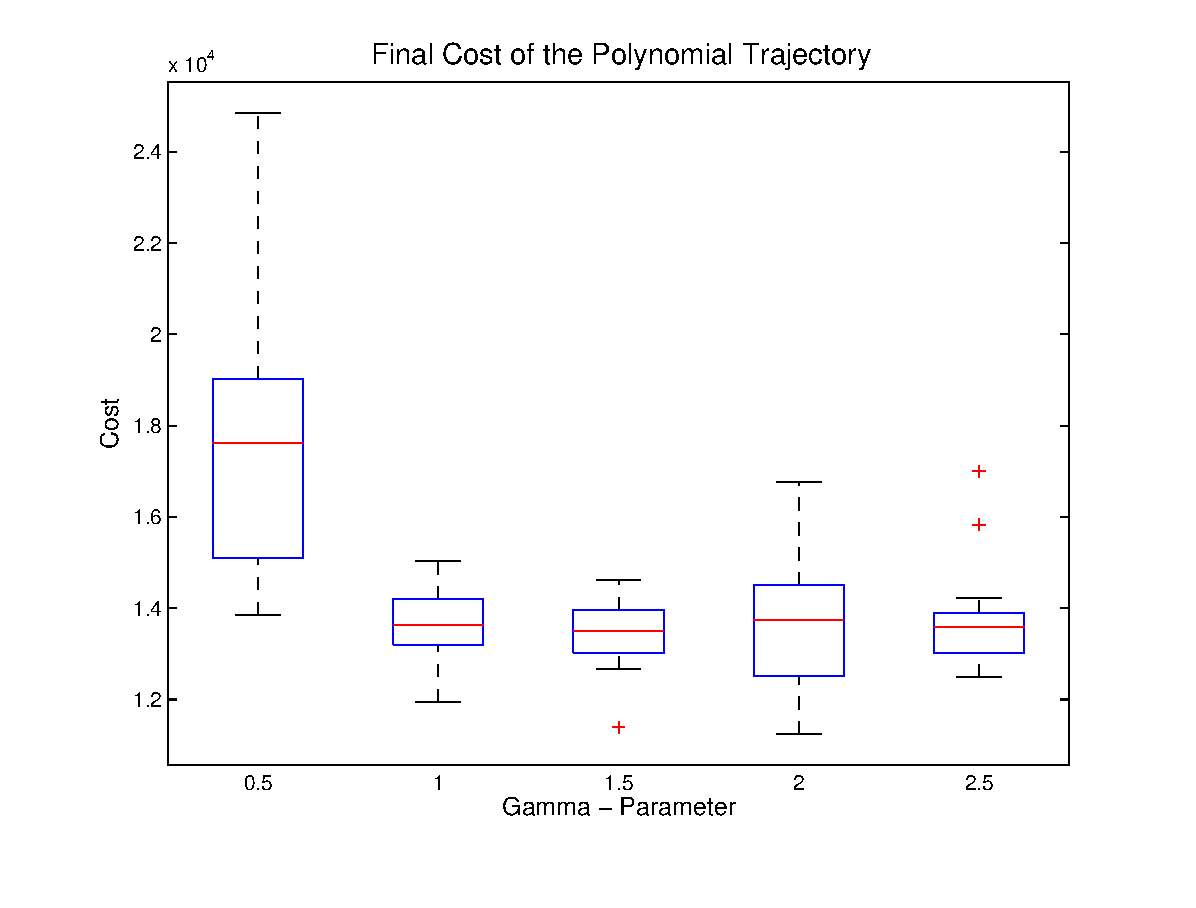
\includegraphics[trim = 14mm 10mm 15mm 0mm,clip,width=1\textwidth]{pics/boxplot1.eps}
%   \caption{The $x$-axis depicts different $\gamma$ parameters and the $y$-axis depicts the final cost of the polynomial trajectory. The red mark illustrates the median. }
%   \label{pic:boxplot}
%\end{figure}
%
%
%It becomes apparent that the small amount of rewiring associated with $\gamma = 0.5$ is to little to obtain a good polynomial trajectory. The 4 remaining datasets have a similar performance in terms of the final trajectory cost. \newline
%
%The total computational times for the five different $\gamma$ parameters are depicted in figure \ref{pic:boxplot_time}. The total computational time is the combined duration of the RRT* algorithm and the nonlinear optimization.  In contrast to the final cost, the total computational times for $\gamma = 1 $, $\gamma = 1.5$, $\gamma = 2$ and $\gamma = 2.5$ are distinct. 
%
%\begin{figure}[H]
%   \centering
%   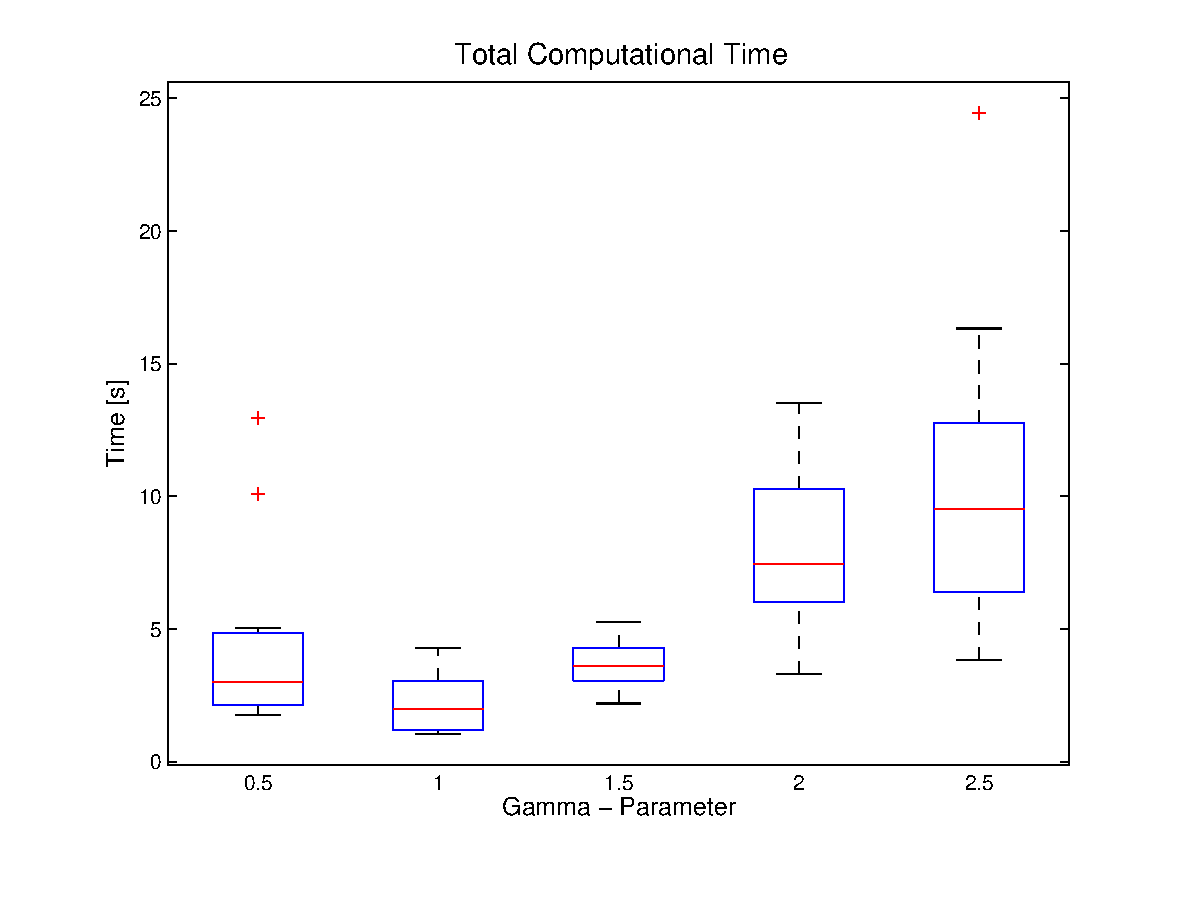
\includegraphics[trim = 14mm 10mm 15mm 0mm,clip,width=1\textwidth]{pics/boxplot_time.eps}
%   \caption{The $x$-axis depicts different $\gamma$ parameters and the $y$-axis depicts the total computational time. The red mark illustrates the median.}
%   \label{pic:boxplot_time}
%\end{figure}
%
%Figure \ref{pic:boxplot_time} shows that the computational time increases significant if $\gamma$ is larger than 1.5. This is simply because the RRT* algorithm needs more time for rewiring. Furthermore, $\gamma = 0.5$ (which is not a good choice sine the final cost is too high) has 2 outliers. In this 2 cases the straight line solution is not enough target-orientated and multible vertex extensions are required to obtain a collision-free trajectory. \newline
%
%Combining the results from figure \ref{pic:boxplot} and figure \ref{pic:boxplot_time}, a $\gamma$ parameter in the range of 1 to 1.5 lead to the best performance.




%
%\begin{figure}
%\centering
%\begin{subfigure}{.5\textwidth}
%  \centering
%  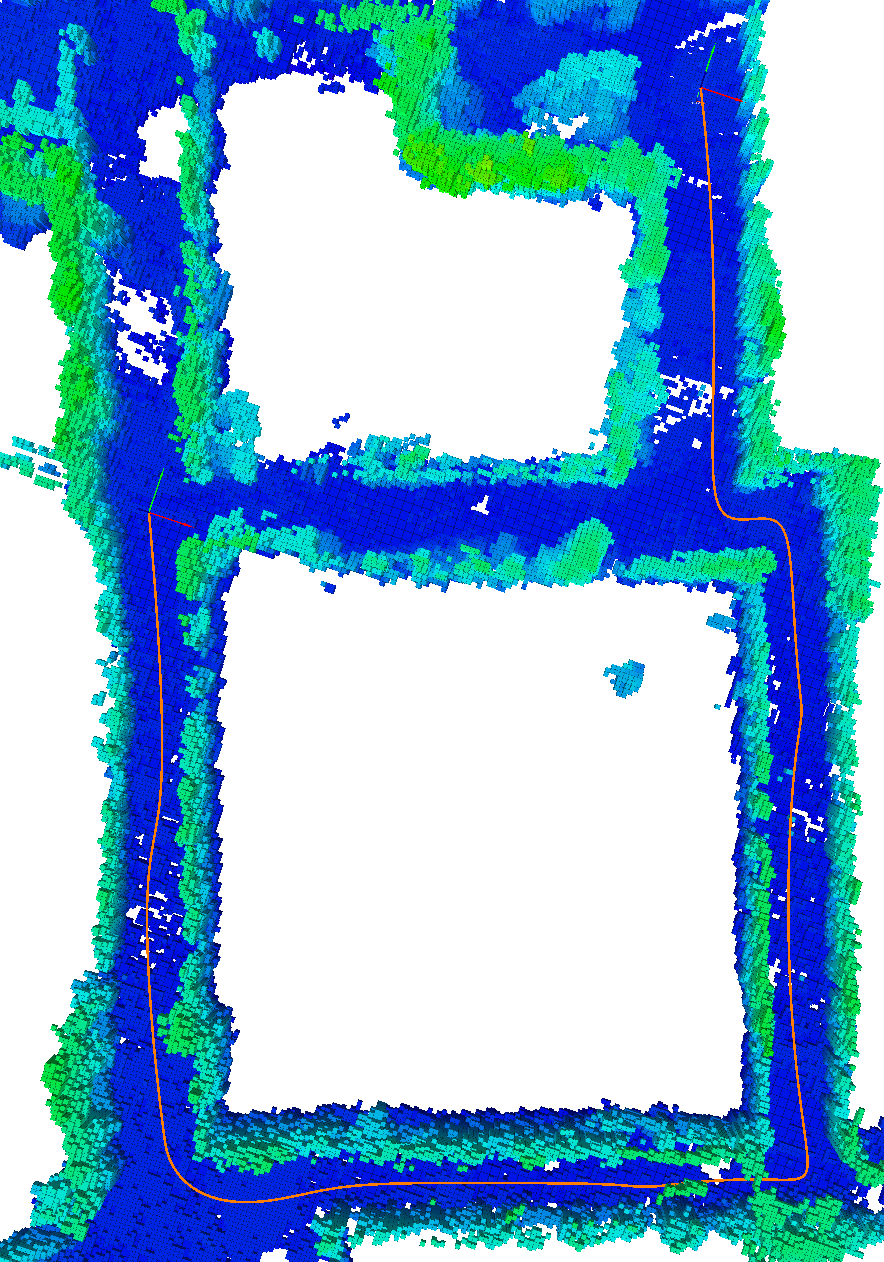
\includegraphics[width=1\linewidth]{pics/MapPoly.png}
%  \caption{A subfigure}
%  \label{fig:sub1}
%\end{subfigure}%
%\begin{subfigure}{.5\textwidth}
%  \centering
%  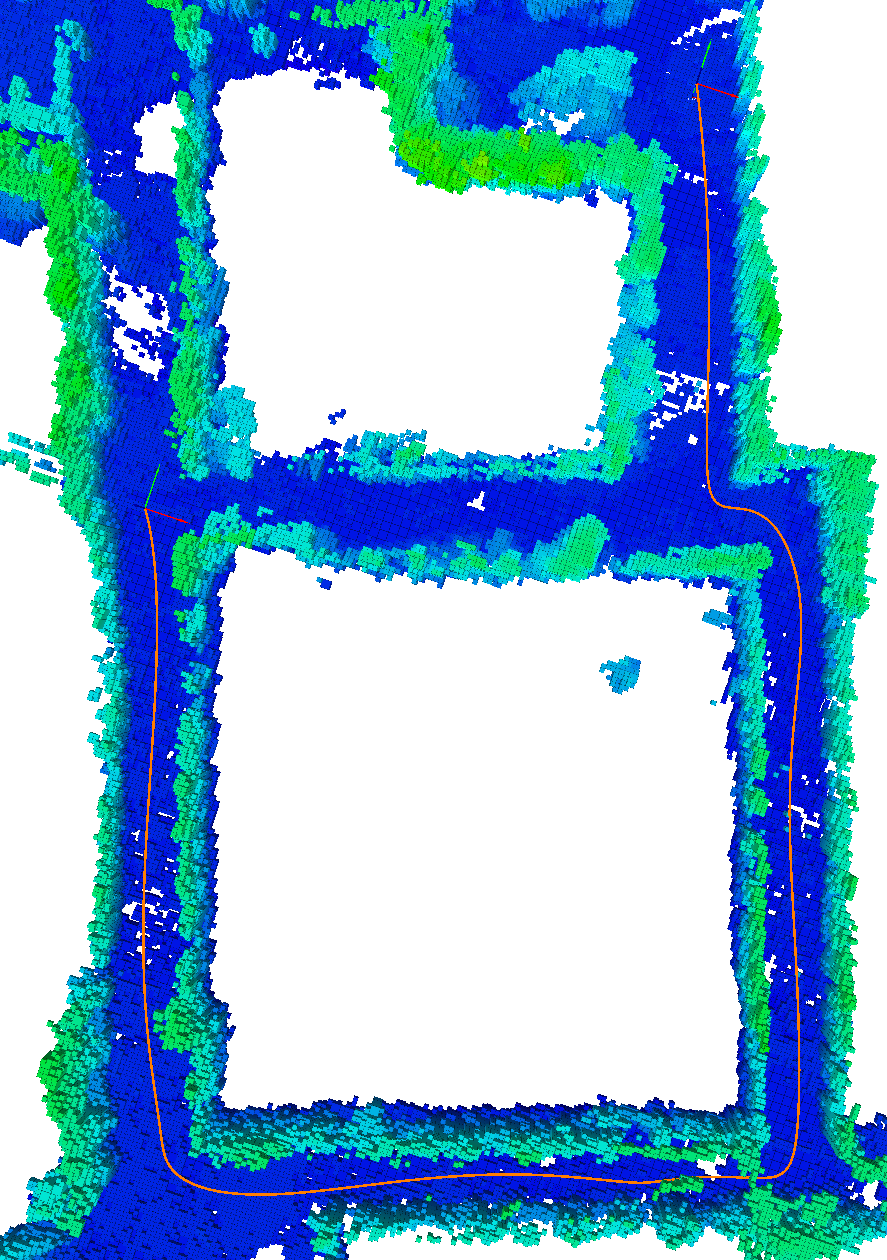
\includegraphics[width=1\linewidth]{pics/MapNlopt.png}
%  \caption{A subfigure}
%  \label{fig:sub2}
%\end{subfigure}
%\caption{A figure with two subfigures}
%\label{fig:test}
%\end{figure}


 \cleardoublepage
%   \chapter{Flight Test}\label{chap:Flight}


\section{Flight Tests in the Vicon Room}

%\begin{figure}[H]
%   \centering
%   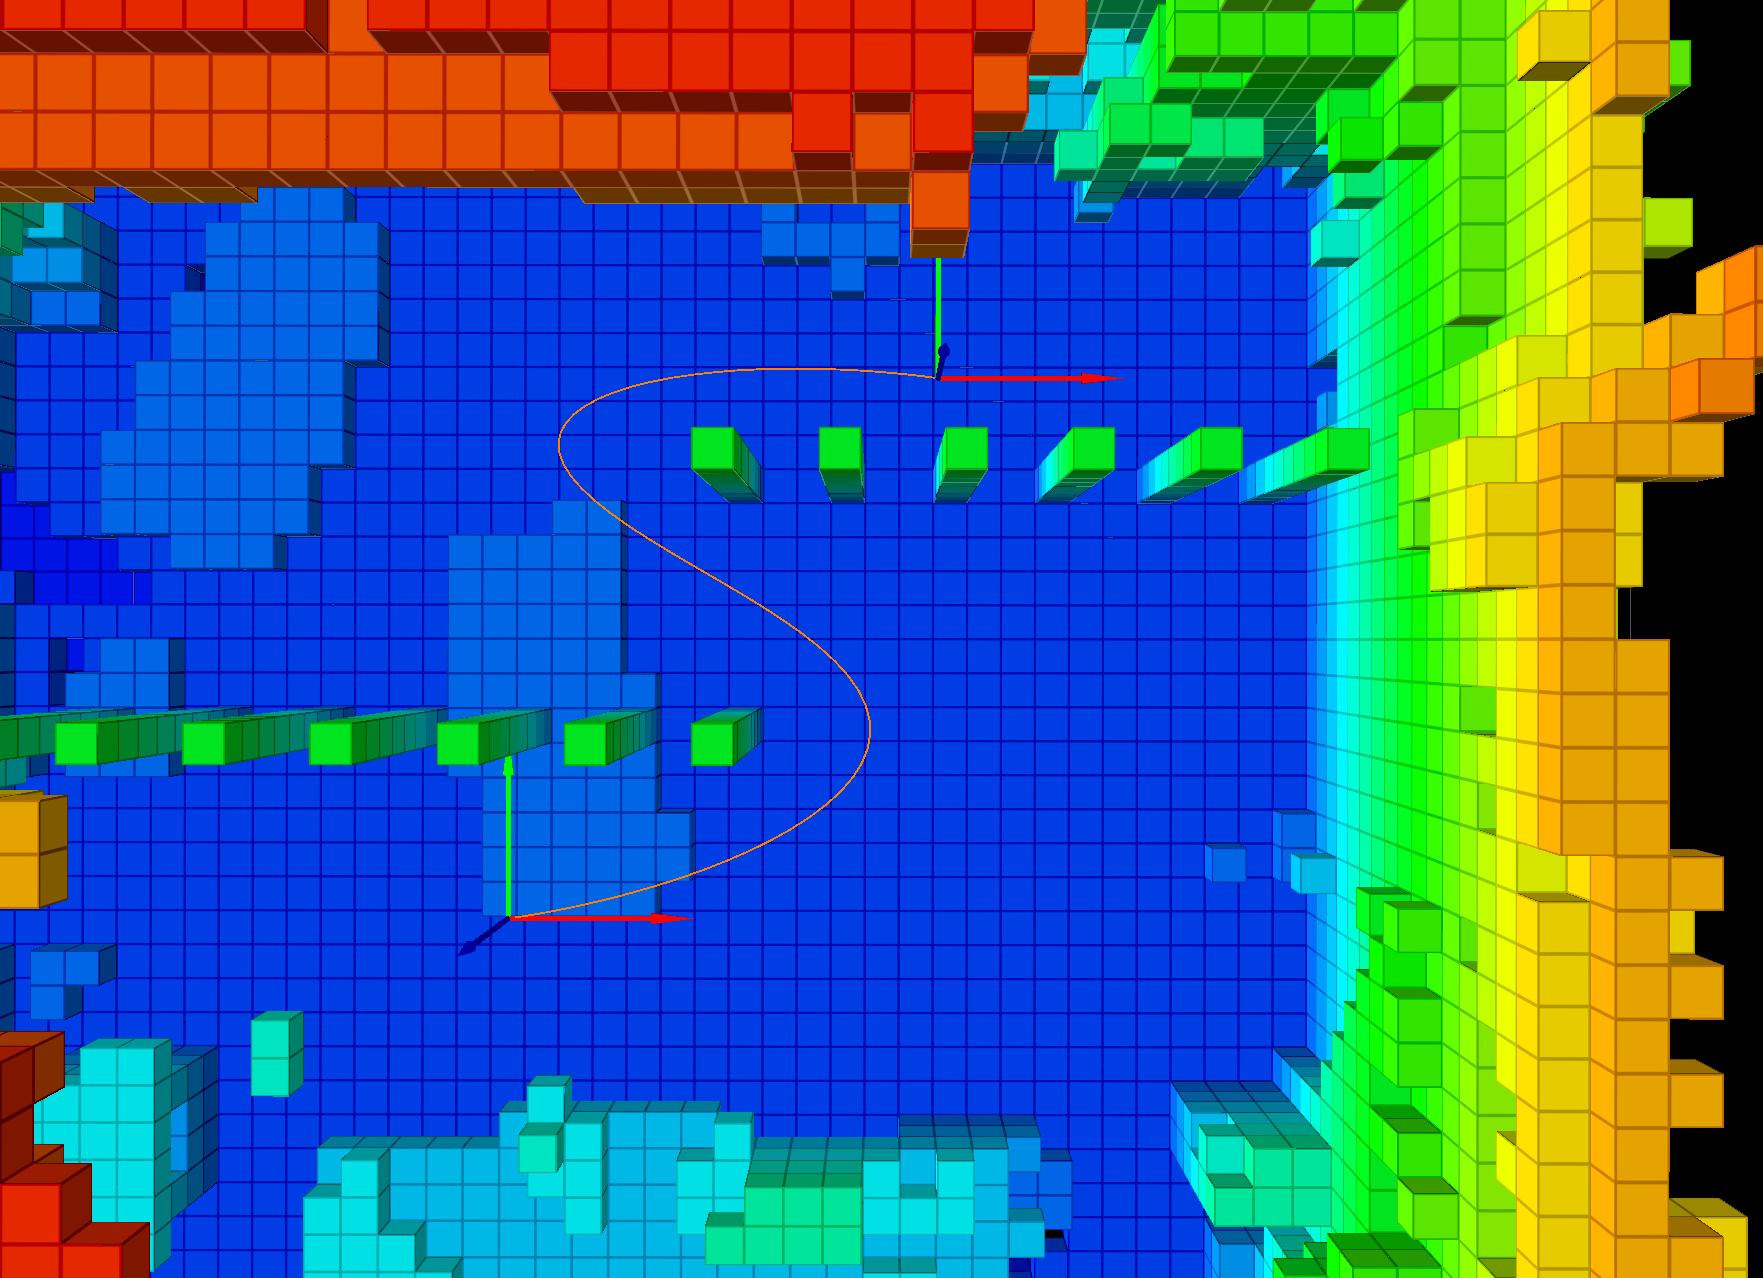
\includegraphics[trim = 0mm 0mm 0mm 0mm,clip,width=1\textwidth]{pics/2b.png}
%   \caption{Bird's eye perspective on hallways in the "ML" building of the ETH Zurich. One start vertex and 6 different goal vertices are depicted}
%   \label{pic:testsfgdsgfdf}
%\end{figure}


\begin{figure}[H]
   \centering
   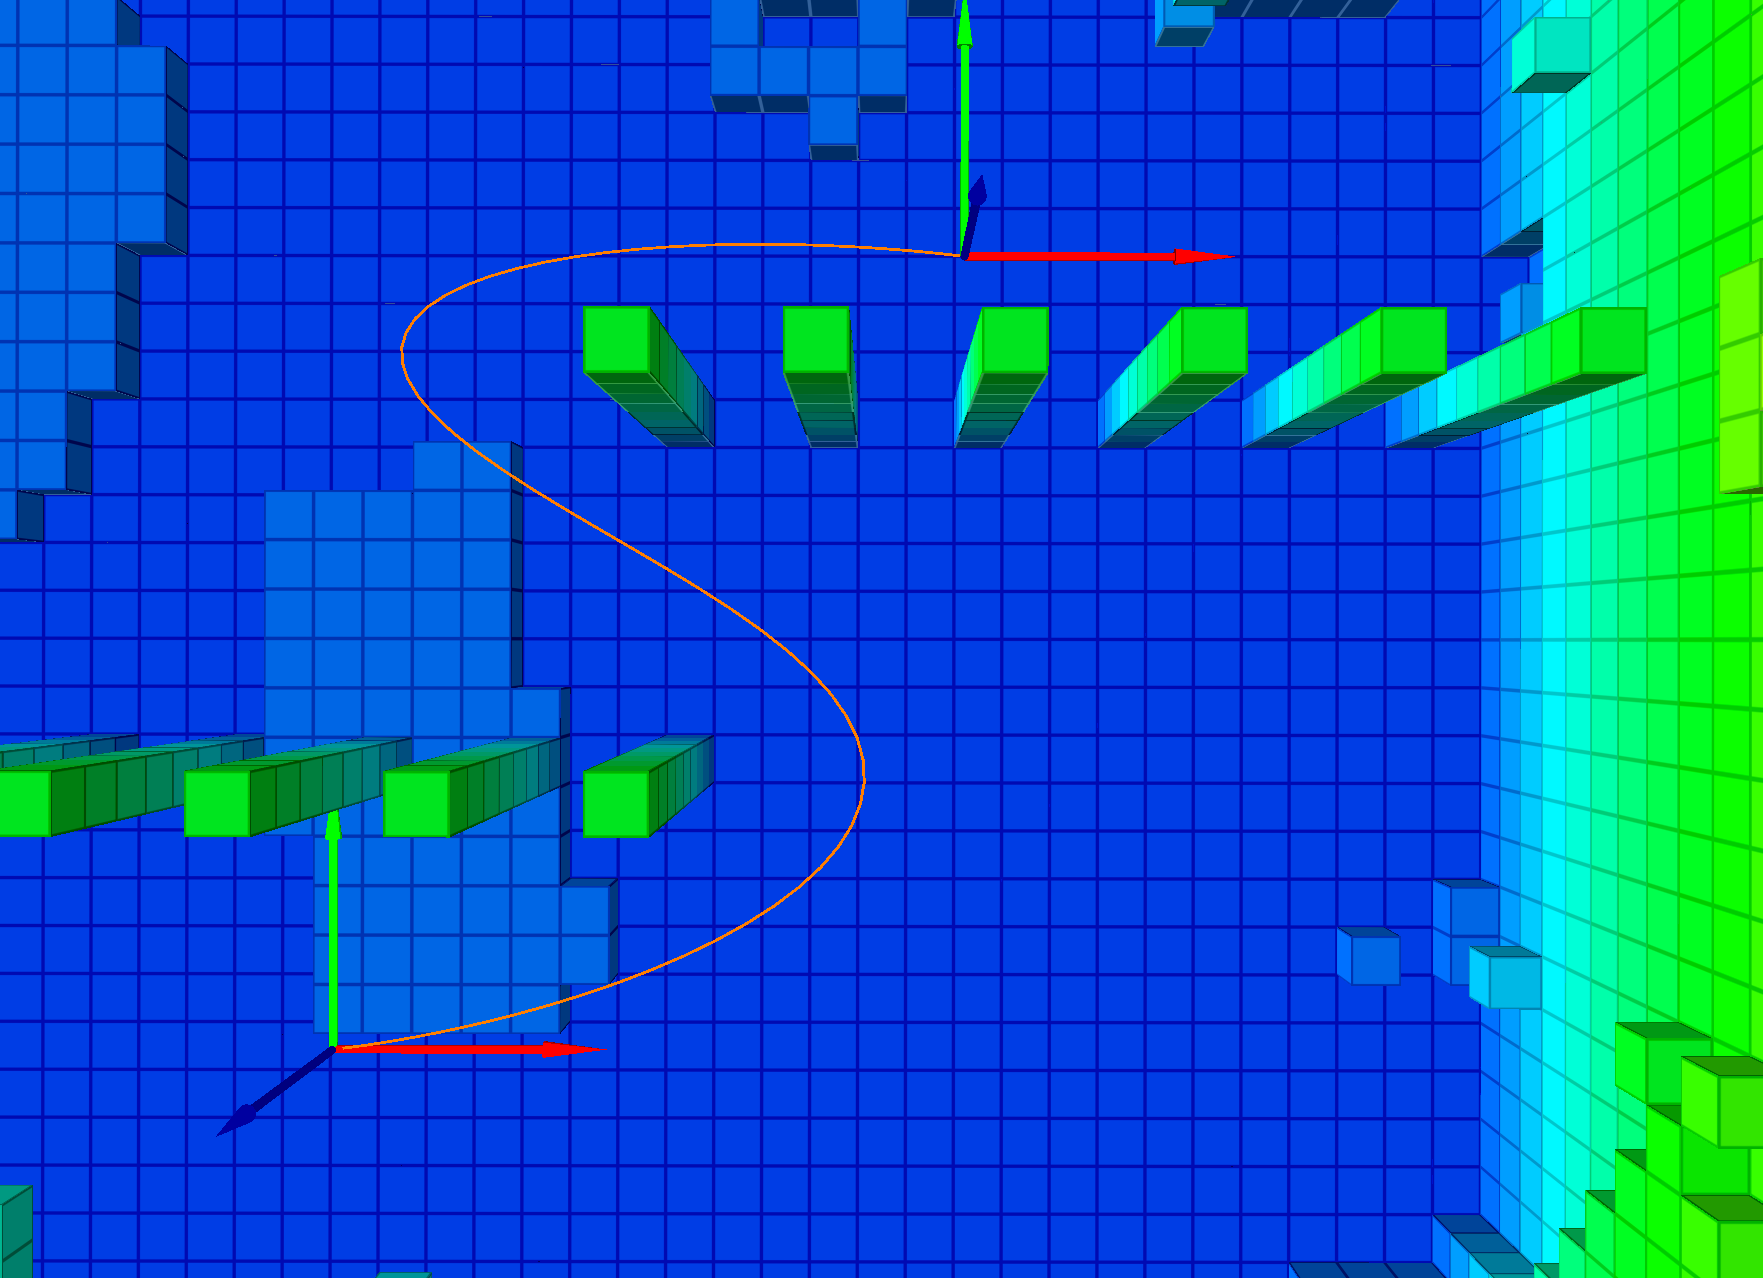
\includegraphics[trim = 0mm 0mm 0mm 0mm,clip,width=1\textwidth]{pics/2c.png}
   \caption{ein bild}
   \label{pic:testdfgd}
\end{figure}




\begin{figure}[H]
   \centering
   \includegraphics[trim = 0mm 0mm 0mm 0mm,clip,width=1\textwidth]{pics/2a.png}
   \caption{ein bild}
   \label{pic:testsfsfsdf}
\end{figure}



%\begin{figure}
%\centering
%\begin{subfigure}{.5\textwidth}
%  \centering
%  \includegraphics[width=1\linewidth]{pics/2a.png}
%  \caption{A subfigure}
%  \label{fig:sub1}
%\end{subfigure}%
%\begin{subfigure}{.5\textwidth}
%  \centering
%  \includegraphics[width=1\linewidth]{pics/2b.png}
%  \caption{A subfigure}
%  \label{fig:sub2}
%\end{subfigure}
%\caption{A figure with two subfigures}
%\label{fig:testsdfaf}
%\end{figure}
% \cleardoublepage
%  \chapter{Conclusion}\label{chap:Conclusion}

The goal of this master thesis was to explore a densely packed environment and then plan a collision-free trajectory for a dynamic UAV flight. \newline

To explore the environment, the RRT* algorithm was applied. The parameters of RRT* have been tuned to serve the subsequent nonlinear optimization in an optimal manner. The vertices of the straight line solution have then been used to generate a polynomial trajectory. Here, the numerical advantages of the unconstrained Quadratic Programming (QP) take full effect. The unconstrained QP has been tested for a large number of optimization variables and is numerical stable for trajectories with more than 2000 segments! \newline

Furthermore, the nonlinear optimization benefits from the numerical stability of the unconstrained QP. The reduction of the optimization variables (i.e. excluding the endpoint derivatives $d_P$ from the cost function) led to a even better performance. The nonlinear optimization has been successfully tested for a trajectory with 200 segments. The NLopt ending criteria was $J_{rel} = 0.5$ and the algorithm converged. \newline

Flight tests in the ETH Vicon room have shown that the path planning algorithm is suitable for online planning. The UAV flew on a smooth, snap minimized trajectory from the current position between multiple obstacles to the user-specified goal position. The current position, which is also used by the controller, is provided by the Vicon motion tracking system. 





% \cleardoublepage
  \chapter{Future Work}\label{chap:Future}

\section{Segment Times of the Initial Solution}
As mentioned in section  \ref{sec:drawbackInitial}, the segment time calculation of the initial solution does not incorporate the circumstances from one segment to another. Hence, the segment time ratio is not optimal. \newline

If a segment has a similar orientation as the previous segment, the required segment time is generally shorter. On the other hand, if there are great changes in the orientation from one segment to another more time is required. If this characteristics are represented in the segment time calculation, unnecessary sharp corners and detours (as depicted in figure \ref{pic:initiSpace}) could be avoided.

\section{Straight Line Characteristics}

In section \ref{sec:dynamicRec} it is explained, that additional RRT* iterations are performed after a collision-free straight line solution has been found. During this additional iterations the straight line solution can be improved via rewiring. The criterion for the improvement is the total length of the straight line segments. \newline
A short straight line solution does not necessarily lead to a god polynomial solution. If the RRT* cost criterion considers any parameters which are connected to the polynomial trajectory, a more suitable straight line solution could be found.

\section{Improvement of the Ray Check}\label{sec:furureRayCheck}

As discussed in section \ref{sec:RayCheck}, the Ray Check approach has theoretical advantages compared to the Bounding Box approach. The bounding boxes need a certain amount of overlap to guarantee a collision-free trajectory. Hence, several cells of the OctoMap are checked multiple times. However, the Bounding Box approach performed better in the experimental comparison. \newline

There are some possible improvements of the Ray Check approach. If only one ray is in collision the whole straight line connection is considered in collision. Otherwise,  the rays are checked one after another. Although a key (which represents a cell) appears only once per ray it is possible that a key is check several times for different rays. The keys of each ray are stored in a list. Of course it is possible to check if a key of a new ray was already an element of an old ray. This method was tested during this master thesis but the performance strongly decreased. 

This is due to the fact, that the keys are complex structures (and not only integers or floating point numbers) which can not be stored in ascending order. That makes it difficult to find a particular key in the list of the old ray. \newline

If it is possible to speed up the procedure of refinding the keys or to find a better solution to store them in an organized manner, a Ray Check algorithm which outperforms the Bounding Box approach is feasible.

\section{Improvement of the Boundig Box}\label{sec:furureBoundingBox}

The above mentioned overlap of the bounding boxes could be reduced if the bounding boxes are oriented properly. At the moment, the bounding box is implemented as a cuboid with its edges aligned to the coordinate system of the map. It would be advantageous if the bounding boxes were aligned to the straight line connection. As a result, no overlap is required to check a RRT* straight line solution. 

\section{Improvement of the Nonlinear Optimization}\label{sec:furureNonOpt}

In section \ref{sec:CompDiffApp} it was demonstrated that the optimization approach with a reduced number of optimization variables (approach B) has a superior performance compared to the approach with the full set of optimization variables (approach A).  \newline

It would be welcome if the nonlinear optimization would reach the global minimum cost of a trajectory with several segments in a reasonable time. Since this was not achieved using NLopt, applying a different nonlinear optimization library is worth a try.

\section{Feasibility of the Trajectory}

Speaking of multi-copter control, the input parameters for the controller are often the thrust $f$ (normalized by the mass) and the body rates $\omega = (\omega_1, \omega_2, \omega_3)$ defined in the body-fixed frame. As explained in the paper from Mark Mueller et al. \cite{mueller}, $\omega_1$ (around $x$-axis) and $\omega_2$ (around $y$-axis) are defined by the thrust $f$, the jerk $j$ and a mapping matrix $R$ from body frame to the inertial frame:

\begin{equation}
\begin{bmatrix}
   \omega_2 \\
  -\omega_1 \\
0
\end{bmatrix}
= \frac{1}{f}
\begin{bmatrix}
   1 & 0  &0\\
  0 & 1 & 0\\
0 & 0 &0
\end{bmatrix}
R^{-1}j
\label{equ:mueller}
\end{equation}


The optimization in this master thesis does not consider the orientation of the UAV. Therefore, no mapping from the body to the inertial frame is possible. Consequently, the values of $\omega$ can not be checked on limitations. \newline

If the thrust $f$ is small, it is hard to reach the desired body rates $\omega$. Since the UAV needs an acceleration of $9.81 \frac{m}{s^2}$ to hover, the trust is only 0 if the UAV is in a free fall. 
The acceleration in this master thesis is calculated excluding the gravity. I.e. a maximum acceleration of $4 \frac{m}{s^2}$ requires an actual acceleration of $13.81 \frac{m}{s^2}$ in the $z$-direction. Simultaneously, the UAV can not fall with an acceleration higher than $5.81 \frac{m}{s^2}$. In other words, an acceleration limit which is smaller than $g$ prevents small thrust values. However, checking the body rates would provide extra information and additional security.




 \cleardoublepage
 %
\chapter{Einige wichtige Hinweise zum Arbeiten mit \LaTeX\ }\label{sec:latexumg}

Nachfolgend wird die Codierung einiger oft verwendeten Elemente
kurz beschrieben. Das Einbinden von Bildern ist in \LaTeX\ nicht
ganz unproblematisch und h�ngt auch stark vom verwendeten Compiler
ab. Typisches Format f�r Bilder in \LaTeX\ ist
EPS\footnote{Encapsulated Postscript}.


\section{Gliederungen}\label{sec:gliederung}

Ein Text kann mit den Befehlen \texttt{\textbackslash
chapter\{.\}}, \texttt{\textbackslash section\{.\}},
\texttt{\textbackslash subsection\{.\}} und \texttt{\textbackslash
subsubsection\{.\}} gegliedert werden.


\section{Referenzen und Verweise}\label{sec:refverw}

Literaturreferenzen werden mit dem Befehl \texttt{\textbackslash
cite\{.\}} erzeugt. Ein Beispiel: \cite{comfilt}.

Zur Erzeugung von Fussnoten wird der Befehl \texttt{\textbackslash
footnote\{.\}} verwendet. Auch hier ein Beispiel\footnote{Bla
bla.}.

Querverweise im Text werden mit \texttt{\textbackslash label\{.\}}
verankert und mit \texttt{\textbackslash ref\{.\}} erzeugt.
Beispiel einer Referenz auf das zweite Kapitel:
Kapitel~\ref{sec:latexumg}.


\section{Aufz�hlungen}\label{sec:aufz}

Folgendes Beispiel einer Aufz�hlung ohne Numerierung,
\begin{itemize}
  \item Punkt 1
  \item Punkt 2
\end{itemize}
wurde erzeugt mit:
\begin{verbatim}
\begin{itemize}
  \item Punkt 1
  \item Punkt 2
\end{itemize}
\end{verbatim}

Folgendes Beispiel einer Aufz�hlung mit Numerierung,
\begin{enumerate}
  \item Punkt 1
  \item Punkt 2
\end{enumerate}
wurde erzeugt mit:
\begin{verbatim}
\begin{enumerate}
  \item Punkt 1
  \item Punkt 2
\end{enumerate}
\end{verbatim}

Folgendes Beispiel einer Auflistung,
\begin{description}
  \item[P1] Punkt 1
  \item[P2] Punkt 2
\end{description}
wurde erzeugt mit:
\begin{verbatim}
\begin{description}
  \item[P1] Punkt 1
  \item[P2] Punkt 2
\end{description}
\end{verbatim}


\section{Erstellen einer Tabelle}\label{sec:tabellen}

Ein Beispiel einer Tabelle:
\begin{table}[h]
\begin{center}
 \caption{Daten der Fahrzyklen ECE, EUDC, NEFZ.}\vspace{1ex}
 \label{tab:tabnefz}
 \begin{tabular}{ll|ccc}
 \hline
 Kennzahl & Einheit & ECE & EUDC & NEFZ \\ \hline \hline
 Dauer & s & 780 & 400 & 1180 \\
 Distanz & km & 4.052 & 6.955 & 11.007 \\
 Durchschnittsgeschwindigkeit & km/h & 18.7 &  62.6 & 33.6 \\
 Leerlaufanteil & \% & 36 & 10 & 27 \\
 \hline
 \end{tabular}
\end{center}
\end{table}

Die Tabelle wurde erzeugt mit:
\begin{verbatim}
\begin{table}[h]
\begin{center}
 \caption{Daten der Fahrzyklen ECE, EUDC, NEFZ.}\vspace{1ex}
 \label{tab:tabnefz}
 \begin{tabular}{ll|ccc}
 \hline
 Kennzahl & Einheit & ECE & EUDC & NEFZ \\ \hline \hline
 Dauer & s & 780 & 400 & 1180 \\
 Distanz & km & 4.052 & 6.955 & 11.007 \\
 Durchschnittsgeschwindigkeit & km/h & 18.7 &  62.6 & 33.6 \\
 Leerlaufanteil & \% & 36 & 10 & 27 \\
 \hline
 \end{tabular}
\end{center}
\end{table}
\end{verbatim}


\section{Einbinden einer EPS-Graphik}\label{sec:epsgraph}

Das Einbinden von Graphiken kann wie folgt bewerkstelligt werden:
\begin{verbatim}
\begin{figure}[h]
   \centering
   \includegraphics[width=0.75\textwidth]{pics/k_surf.eps}
   \caption{Ein Bild.}
   \label{pics:k_surf}
\end{figure}
\end{verbatim}

\begin{figure}[h]
   \centering
   \includegraphics[width=0.75\textwidth]{pics/k_surf.eps}
   \caption{Ein Bild.}
   \label{pics:k_surf}
\end{figure}

oder bei zwei Bildern nebeneinander mit:
\begin{verbatim}
\begin{figure}[h]
  \begin{minipage}[t]{0.48\textwidth}
    \includegraphics[width = \textwidth]{pics/cycle_we.eps}
  \end{minipage}
  \hfill
  \begin{minipage}[t]{0.48\textwidth}
    \includegraphics[width = \textwidth]{pics/cycle_ml.eps}
  \end{minipage}
  \caption{Zwei Bilder nebeneinander.}
  \label{pics:cycle}
\end{figure}
\end{verbatim}

\begin{figure}[h]
  \begin{minipage}[t]{0.48\textwidth}
    \includegraphics[width = \textwidth]{pics/cycle_we.eps}
  \end{minipage}
  \hfill
  \begin{minipage}[t]{0.48\textwidth}
    \includegraphics[width = \textwidth]{pics/cycle_ml.eps}
  \end{minipage}
  \caption{Zwei Bilder nebeneinander.}
  \label{pics:cycle}
\end{figure}

Bemerkung: Ersetzt man den Positionierungsparameter \texttt{h}
durch \texttt{H}, so wird das Gleiten der Abbildung verhindert.


\section{Mathematische Formeln}\label{sec:math}

Einfache mathematische Formeln werden mit der equation-Umgebung
erzeugt:
\begin{equation}
 p_{me0f}(T_e,\omega_e) \ = \ k_1(T_e) \cdot (k_2+k_3 S^2
 \omega_e^2) \cdot \Pi_{max} \cdot \sqrt{\frac{k_4}{B}} \, .
\end{equation}

Der Code dazu lautet:
\begin{verbatim}
\begin{equation}
 p_{me0f}(T_e,\omega_e) \ = \ k_1(T_e) \cdot (k_2+k_3 S^2
 \omega_e^2) \cdot \Pi_{max} \cdot \sqrt{\frac{k_4}{B}} \, .
\end{equation}
\end{verbatim}

Mathematische Ausdr�cke im Text werden mit \$formel\$ erzeugt (zB:
$a^2+b^2=c^2$).


\section{Weitere n�tzliche Befehle}\label{sec:div}

Hervorhebungen im Text sehen so aus: \emph{hervorgehoben}. Erzeugt
werden sie mit dem \texttt{\textbackslash epmh\{.\}} Befehl.

 %\cleardoublepage
% ...
%
%---------------------------------------------------------------------------
% Appendix

% \appendix
% 
\chapter{Irgendwas}\label{sec:irgendwas}

Bla bla \dots

 \cleardoublepage

%
%\chapter{Nochmals irgendwas}\label{sec:nochirgendwas}
%
%Bla bla \dots
%
% \cleardoublepage

%
%---------------------------------------------------------------------------
% Literature

 
\begin{thebibliography}{99}
%\addcontentsline{toc}{chapter}{Literaturverzeichnis}
\addcontentsline{toc}{chapter}{Bibliography}



\bibitem {he} {\sc R. He, A. Bachrach, M. Achtelik, A. Geramifard, D. Gurdan, S. Prentice,
J. Stumpf, and N. Roy}: 
{\it On the design and use of a micro air
vehicle to track and avoid adversaries}. The Int. Journal of Robotics
Research, vol. 29, pp. 529-546, 2010.


\bibitem {colling} {\sc D. Colling, O. A.~Yakimenko, J. F.~Whidborne, and A. K.~Cooke}:
{\it A prototype of an autonomous controller for a quadrotor UAV}. In
Proceedings of the European Control Conference, Kos, Greece, 2007,
pp. 1-8.


\bibitem {hehn} {\sc M. Hehn and R. D'Andrea }:
{\it Quadrocopter trajectory generation and control}. In
International Federation of Automatic Control (IFAC), World Congress 2011, 2011.


\bibitem {lup} {\sc S. Lupashin, A. Schollig, M. Sherback, and R. D'Andrea}:
 {\it A simple learning strategy for high-speed quadrocopter multi-flips}.
In Proc. of the IEEE Int. Conf. on Robotics and Automation, Anchorage, AK,
May 2010, pp. 1642-1648.


\bibitem {bou} {\sc Y. Bouktir, M. Haddad, and T. Chettibi}:
{\it Trajectory Planning for a
Quadrotor Helicopter}. In Mediterranean Conference on Control and
Automation, Jun. 2008, pp. 1258-1263


\bibitem {mellinger} {\sc D. Mellinger and V. Kumar}: 
{\it Minimum snap trajectory generation and
control for quadrotors}. In International Conference on Robotics and
Automation, 2011, pp. 2520-2525.

\bibitem {lik} {\sc M. Likhachev, G. Gordon and S. Thrun}: 
{\it  ARA*: Anytime A* with Provable Bounds on Sub-Optimality }.
Advances in Neural Information
Processing Systems, vol. 16, 2003

\bibitem {richter} {\sc C. Richter,  A. Bry, and N, Roy}: 
{\it  Polynomial Trajectory Planning
for Quadrotor Flight}.
In International Conference on Robotics and
Automation, 2013.



\end{thebibliography}


%---------------------------------------------------------------------------

\end{document}
%===========================================================================
